\mfpicnumber{1}
\opengraphsfile{1_Linears}

\section{Solving Linear Equations}
\documentclass[11pt]{book}
%\oddsidemargin 0in
%\evensidemargin 0in
%\marginparwidth 0in

%\usepackage[top=1in
%,left=1.5in,
%bottom=1in,%right=1in,textheight=8.5in,textwidth=6in
%]{geometry}

\usepackage{amsfonts,amssymb,amsmath,amsthm,fancyhdr,supertabular,longtable,hhline}
\usepackage{colortbl}
\usepackage{docmute}
\usepackage{import, multicol,boxedminipage}
\usepackage{chapterfolder}
\usepackage[metapost,truebbox]{mfpic}
\usepackage[pdflatex]{graphicx}
\usepackage{graphics}
\usepackage{pgf, tikz}
\usepackage[matrix,arrow,curve]{xy}
\usepackage{setspace}
\usepackage{makeidx}
\usepackage{nomencl}
\usepackage[english]{babel}
\usepackage[colorlinks, hyperindex, plainpages=false, linkcolor=blue, urlcolor=blue, pdfpagelabels]{hyperref}
\usepackage[all]{hypcap}
\usepackage{cancel}
\usepackage{sectsty}
\usepackage{textcomp}
\usepackage{array}
\usepackage{vwcol}
\usepackage{cancel}
\usepackage[
type={CC},
modifier={by-nc-sa},
version={4.0},
]{doclicense}
%\usepackage{bbm}

%First appears in II.1.1
\newcommand{\tmdummy}{$\mbox{}$}
\newcommand{\tmmathbf}[1]{\ensuremath{\boldsymbol{#1}}}
\newcommand{\tmop}[1]{\ensuremath{\operatorname{#1}}}
\newcommand{\tmstrong}[1]{\textbf{#1}}
%{\theorembodyfont{\rmfamily}
%First appears in II.1.?
\newcommand{\tmem}[1]{{\em #1\/}}
%\newenvironment{enumeratenumeric}{\begin{enumerate}[1.] }{\end{enumerate}}
%First appears in II.1.6a
\newenvironment{itemizedot}{\begin{itemize} \renewcommand{\labelitemi}{$\bullet$}\renewcommand{\labelitemii}{$\bullet$}\renewcommand{\labelitemiii}{$\bullet$}\renewcommand{\labelitemiv}{$\bullet$}}{\end{itemize}}


\allsectionsfont{\mdseries \scshape}
\definecolor{ResultColor}{gray}{1.0} %SZ set to gray, 0.9
\theoremstyle{definition}  % this prevents the text in definitions, theorems, and corollaries from being italicized
\newtheorem*{defn}{Definition}%[chapter] % this item asterisked for numbering purposes (across all chapters).
%\newtheorem*{thm}{Theorem}%[chapter] % this item asterisked for numbering purposes (across all chapters).
\newtheorem{thm}{Theorem}[chapter] % this item asterisked for numbering purposes (across all chapters).
\newtheorem*{cor}%[thm]
{Corollary} % this item asterisked for numbering purposes (across all chapters).
\newtheorem{eqn}{Equation}[chapter]
\newtheorem{ex}{Example}[chapter] % this is needed for all Stitz Zeager content.
\newtheorem{example}{Example}[chapter]
\newtheorem{fig}{\sc Figure}[chapter]
\setlength{\parindent}{0in}
\setlength{\extrarowheight}{2pt}
\newcommand{\bbm}{\begin{boxedminipage}{4.80in}} %SZ set to 6.41
\newcommand{\ebm}{\end{boxedminipage}}
\newcounter{HW}
\newcounter{HWindent}

\newcommand{\comment}[1]{}
\newcommand{\pp}{\par~\par}

\begin{document}

\subsection{One-Step Equations}\par
~\par
{\textbf{Objective:}} {\textbf{Solve one-step linear equations by
balancing using inverse operations}}\par
~\par
Solving linear equations is an important and fundamental skill in algebra. In
algebra, we are often presented with a problem where the answer is known, but
part of the problem is missing. The missing part of the problem is what we
seek to find. An example of such a problem is shown below.

\begin{example}\label{Lin1}
\[ 4 x + 16 = - 4 \]
\end{example}
Notice the above problem has a missing part, or unknown, that is marked by
$x$. If we are given that the solution to this equation is $x=- 5$, it could be
plugged into the equation, replacing the $x$ with $- 5$. This is shown in
Example \ref{Lin2}.

\begin{example}\label{Lin2}
\begin{eqnarray*}
  4 (- 5) + 16 = - 4 &  & \tmop{Multiply} 4 (- 5)\\
  - 20 + 16 = - 4 &  & \tmop{Add} - 20 + 16\\
  - 4 = - 4 &  & \tmop{True} !
\end{eqnarray*}
\end{example}

Now the equation comes out to a true statement! Notice also that if another
number, for example, $x=3$, was plugged in, we would not get a true statement as
seen in Example \ref{Lin3}.

\begin{example}\label{Lin3}
 \begin{eqnarray*}
  4 (3) + 16 = - 4 &  & \tmop{Multiply} 4 (3)\\
  12 + 16 = - 4 &  & \tmop{Add} 12 + 16\\
  28 \neq - 4 &  & \tmop{False} !
\end{eqnarray*}
\end{example}
Due to the fact that this is not a true statement, this demonstrates that $x=3$
is not the solution. However, depending on the complexity of the problem, this
``guess and check'' method is not very efficient. Thus, we take a more
algebraic approach to solving equations. Here we will focus on what are called
``one-step equations'' or equations that only require one step to solve. While
these equations often seem very fundamental, it is important to master the
pattern for solving these problems so we can solve more complex problems.\par
~\par

{\textbf{Addition Problems}}\par
~\par

To solve equations, the general rule is to do the opposite, as demonstrated in the following example.

\begin{example}\label{Lin4}
\begin{eqnarray*}
  x + 7 = - 5 &  & \tmop{The} 7 \tmop{is} \tmop{added} \tmop{to} \tmop{the}
  x\\
  ~~~\underline{\tmmathbf{- 7 ~~- 7}} &  & \tmop{Subtract} 7 \tmop{from}
  \tmop{both} \tmop{sides} \tmop{to} \tmop{get} \tmop{rid} \tmop{of}
  \tmop{it}\\
  x = - 12 &  & \tmop{Our} \tmop{solution}
\end{eqnarray*}
\end{example}

It is important for the reader to recognize the benefit of checking an answer by plugging it back into the given equation, as we did with examples \ref{Lin2} and \ref{Lin3} above.  This is a step that often gets overlooked by many individuals who may be eager to attempt the next problem.  As is the case with most textbooks, we will often omit this step from this point forward, with the understanding that it will usually be an exercise that is left to the reader to verify the validity of each answer.\pp

The same process is used in each of the following examples.

\pagebreak

\begin{example}\label{Lin5}
~\end{example}

	\begin{table}[h]
		\begin{tabular}{l}
    ~~~$4 + x = 8$\\
    \underline{$\ensuremath{\boldsymbol{- 4 ~~~~~~~- 4}}$}~~~~\\
    ~~~~ $x = 4$
  \end{tabular} \ \ \ \ \ \ \ \ \ \ \ \ \ \ \ \ \ \ \ \begin{tabular}{l}
    \ \ $7 = x + 9$\\
    $\tmmathbf{\underline{- 9 ~~~~- 9}}$\\
    ~~~~ $- 2 = x$
  \end{tabular} \ \ \ \ \ \ \ \ \ \ \ \ \ \ \ \ \ \ \ \begin{tabular}{l}
    \ \ ~~$5 = 8 + x$\\
    $\tmmathbf{\underline{- 8 ~~- 8}}$\\
    ~~~~ $- 3 = x$
  \end{tabular}
  \caption{Addition Examples}
	\end{table}
%\end{example}

%\pagebreak

{\textbf{Subtraction Problems}}\par
~\par
In a subtraction problem, we get rid of negative numbers by adding them to
both sides of the equation, as demonstrated in the following example.

\begin{example}\label{Lin6}
  \begin{eqnarray*}
    x - 5 = 4~~~ &  & \tmop{The} 5 \tmop{is} \tmop{negative}, \tmop{or}
    \tmop{subtracted} \tmop{from} x\\
    ~~~~~~\tmmathbf{\underline{+ 5 ~~+ 5}} &  & \tmop{Add} 5 \tmop{to} \tmop{both}
    \tmop{sides}\\
    x = 9\qquad  &  & \tmop{Our} \tmop{solution}
  \end{eqnarray*}
\end{example}

The same process is used in each of the following examples. Notice that each time we are getting rid of a negative
number by adding.\pp
In every example, we introduce the opposite operation of what is shown, in order to solve the given equation.  This notion of opposites is more commonly referred to as an \textit{inverse} operation.  The inverse operation of addition is subtraction, and vice versa.  Similarly, the inverse operation of multiplication is division, and vice versa, which we will see momentarily.

\begin{example}\label{Lin7}
~\end{example}

  \begin{table}[h]
    \begin{tabular}{l}
      $- 6 + x = - 2$\\
      $\tmmathbf{\underline{+ 6 ~~~~~~~+ 6}}$\\
      ~~~~ $x = 4$
    \end{tabular} \begin{tabular}{l}
      
    \end{tabular}\begin{tabular}{l}
      
    \end{tabular} \ \ \ \ \ \ \ \ \ \ \ \ \ \ \ \ \ \ \begin{tabular}{l}
      $- 10 = x - 7$\\
      $ \tmmathbf{\underline{+ 7 ~~~~~~~+ 7}}$\\
      ~~~~ $- 3 = x$
    \end{tabular} \ \ \ \ \ \ \ \ \ \ \ \ \ \ \ \ \ \ \ \begin{tabular}{l}
      ~~~$5 = - 8 + x$\\
      ~$\tmmathbf{\underline{+ 8 ~~~+ 8}}$\\
      ~~~~ $13 = x$
    \end{tabular}
    \caption{Subtraction Examples}
  \end{table}
%\end{example}

{\textbf{Multiplication Problems}}\par
~\par
With a multiplication problem, we get rid of the number by dividing on both
sides, as demonstrated in the following examples.

\begin{example}\label{Lin8}
  \begin{eqnarray*}
    4 x = 20 ~~&  & \tmop{Variable} \tmop{is} \tmop{multiplied} \tmop{by} 4\\
    ~~~\tmmathbf{\overline{4} ~~~~~ \overline{4}}~~ &  & \tmop{Divide} \tmop{both}
    \tmop{sides} \tmop{by} 4\\
    x = 5~~ &  & \tmop{Our} \tmop{solution}
  \end{eqnarray*}
\end{example}

With multiplication problems it is very important that care is taken with
signs. If $x$ is multiplied by a negative then we will divide by a negative.
This is shown in example \ref{Lin9}.

\begin{example}\label{Lin9}
  \begin{eqnarray*}
    - 5 x = 30 &  & \tmop{Variable} \tmop{is} \tmop{multiplied} \tmop{by} -
    5\\
    \tmmathbf{\overline{- 5} ~~~~ \overline{- 5}} &  & \tmop{Divide} \tmop{both}
    \tmop{sides} \tmop{by} - 5\\
    x = - 6 &  & \tmop{Our} \tmop{solution}
  \end{eqnarray*}
\end{example}

The same process is used in each of the following examples. Notice how
negative and positive numbers are handled as each problem is solved.

\begin{example}\label{Lin10}
~\end{example}
 
 \begin{table}[h]
    \begin{tabular}{l}
      $8 x = - 24$\\
      $\tmmathbf{\overline{8} ~~~~~~~~ \overline{8}}$\\
      ~~~~ $x = - 3$
    \end{tabular} \ \ \ \ \ \ \ \ \ \ \ \ \ \ \ \ \ \ \ \begin{tabular}{l}
      $- 4 x = - 20$\\
      \ $\tmmathbf{\overline{- 4} ~~~~~ \overline{- 4}}$\\
      ~~~~ $x = 5$
    \end{tabular} \ \ \ \ \ \ \ \ \ \ \ \ \ \ \ \ \ \ \ \begin{tabular}{l}
      $42 = 7 x$~~\\
      ~$\tmmathbf{\overline{7} ~~~~~ \overline{7}}$\\
      ~~~~ $6 = x$
    \end{tabular}
    \caption{Multiplication Examples}
  \end{table}
%\end{example}

{\textbf{Division Problems}}\par
~\par
In division problems, we get rid of the denominator by multiplying on both
sides, since multiplication is the opposite, or \textit{inverse}, operation of division. This is demonstrated in the examples shown below.

\begin{example}\label{Lin11}
  \begin{eqnarray*}
    \frac{x}{5} = - 3 &  & \tmop{Variable} \tmop{is} \tmop{divided} \tmop{by}
    5\\
    \tmmathbf{(5)} \frac{x}{5} = - 3 \tmmathbf{(5)} &  & \tmop{Multiply}
    \tmop{both} \tmop{sides} \tmop{by} 5\\
    x = - 15 &  & \tmop{Our} \tmop{solution}
  \end{eqnarray*}
\end{example}

Then we get our solution $x = - 15$. %The same process is used in each of the
%following examples.

\pagebreak

\begin{example}\label{Lin12}
~\end{example}

\begin{table}[h]
  \begin{tabular}{l}
    $ \frac{x}{- 7} = - 2$\\
    $\tmmathbf{(-7)}\frac{x}{- 7} = - 2\tmmathbf{(-7)}$\\
    ~~~~ $x = 14$
  \end{tabular} \ \ \ \ \ \ \ \ \ \ \ \ \ \ \begin{tabular}{l}
    $ \frac{x}{8} = 5$\\
    $\tmmathbf{(8)} \frac{x}{8} = 5 \tmmathbf{(8)}$\\
    ~~~~ $x = 40$
  \end{tabular} \ \ \ \ \ \ \ \ \ \ \ \ \ \ \begin{tabular}{l}
    $ \frac{x}{- 4} = 9$\\
    $\tmmathbf{(-4)}\frac{x}{- 4} = 9\tmmathbf{(-4)}$\\
    ~~~~ $x = - 36$
  \end{tabular}
  \caption{Division Examples}
\end{table}
%\end{example}

The process described above is fundamental to solving equations. Once this
process is mastered, the problems we will see have several more steps. These
problems may seem more complex, but the process and patterns used will remain
the same.\pp
{\textbf{World View Note: }}The study of algebra originally was called the
``Cossic Art'' \ from the Latin, the study of ``things'' (which we now call
variables).
\end{document}
\newpage
\subsection{Two-Step Equations}\pp

 {\tmstrong{Objective: Solve two-step equations by balancing and using inverse
operations.}}\pp

 After mastering the technique for solving one-step equations, we are ready to consider two-step equations. As we solve two-step
equations, the important thing to remember is that everything works backwards!
When working with one-step equations, we learned that in order to clear a
``plus five'' in the equation, we would subtract five from both sides. We
learned that to clear ``divided by seven'' we multiply by seven on both sides.
The same pattern applies to the order of operations. When solving for our
variable $x$, we use order of operations backwards as well. This means we will
add or subtract first, then multiply or divide second (then exponents, and
finally any parentheses or grouping symbols, but that's another lesson).

\begin{example}\label{Lin13}
   
  \begin{eqnarray*}
    4 x - 20 = - 8 &  & 
  \end{eqnarray*}
   We have two numbers on the same side as the $x$. We need to move the $4$ and
  the $20$ to the other side. We know to move the $4$ we need to divide, and
  to move the $20$ we will add $20$ to both sides. If order of operations
  is done backwards, we will add or subtract first. Therefore we will add $20$
  to both sides first. Once we are done with that, we will divide both sides
  by $4$. The steps are shown below.
  \begin{eqnarray*}
    4 x - 20 = - 8~~ &  & \tmop{Start} \tmop{by} \tmop{focusing} \tmop{on}
    \tmop{the} \tmop{subtract} 20\\
    \tmmathbf{\underline{+ 20 ~~+ 20}} &  & \tmop{Add} 20 \tmop{to} \tmop{both}
    \tmop{sides}\\
    4 x = 12~~ &  & \tmop{Now} \tmop{we} \tmop{focus} \tmop{on} \tmop{the} 4
    \tmop{multiplied} \tmop{by} x\\
    \tmmathbf{\overline{4} ~~~~~ \overline{4}~}~ &  & \tmop{Divide} \tmop{both}
    \tmop{sides} \tmop{by} 4\\
    x = 3~~ &  & \tmop{Our} \tmop{solution}
  \end{eqnarray*}
\end{example}

 Notice in our next example when we replace the $x$ with $3$ \ we get a true
statement.
\begin{eqnarray*}
  4 (3) - 20 = - 8 &  & \tmop{Multiply} 4 (3)\\
  12 - 20 = - 8 &  & \tmop{Subtract} 12 - 20\\
  - 8 = - 8 &  & \tmop{True} !
\end{eqnarray*}
 The same process is used to solve any two-step equation. Add or subtract
first, then multiply or divide.

\begin{example}\label{Lin14}
  
  \begin{eqnarray*}
    5 x + 7 = 7~~ &  & \tmop{Start} \tmop{by} \tmop{focusing} \tmop{on}
    \tmop{the} \tmop{plus} 7\\
    \tmmathbf{\underline{- 7 ~~- 7}} &  & \tmop{Subtract} 7 \tmop{from}
    \tmop{both} \tmop{sides}\\
    5 x = 0~~ &  & \tmop{Now} \tmop{focus} \tmop{on} \tmop{the}
    \tmop{multiplication} \tmop{by} 5\\
    \tmmathbf{\overline{5} ~~~~~ \overline{5}}~~ &  & \tmop{Divide} \tmop{both}
    \tmop{sides} \tmop{by} 5\\
    x = 0~~ &  & \tmop{Our} \tmop{solution}
  \end{eqnarray*}
\end{example}

Notice the seven subtracted out completely! Many students get stuck on this
point, do not forget that we have a number for ``nothing left'', and that
number is zero. With this in mind the process is almost identical to our first
example.\pp

 A common error students make with two-step equations is with negative signs.
Remember the sign always stays with the number. Consider the following
example.

\begin{example}\label{Lin15}
 
   \begin{eqnarray*}
    4 - 2 x = 10 &  & \tmop{Start} \tmop{by} \tmop{focusing} \tmop{on}
    \tmop{the} \tmop{positive} 4\\
    \underline{\tmmathbf{- 4 ~~~~~~- 4}} &  & \tmop{Subtract} 4 \tmop{from}
    \tmop{both} \tmop{sides}\\
    - 2 x = 6~~ &  & \tmop{Negative~} (\tmop{subtraction}) \tmop{~stays} \tmop{on}
    \tmop{the} 2 x\\
    \tmmathbf{\overline{- 2} ~~~ \overline{- 2}} &  & \tmop{Divide} \tmop{by} -
    2\\
    x = - 3 &  & \tmop{Our} \tmop{solution}
  \end{eqnarray*}
\end{example}

 The same is true even if there is no apparent coefficient in front of the variable.  The coefficient is $1$ or $-1$ in this case.
Consider the next example.

\begin{example}\label{Lin16}
 
  
  \begin{eqnarray*}
    8 - x = 2~ &  & \tmop{Start} \tmop{by} \tmop{focusing} \tmop{on} \tmop{the}
    \tmop{positive} 8\\
    \tmmathbf{\underline{- 8 ~~~~~- 8}} &  & \tmop{Subtract} 8 \tmop{from}
    \tmop{both} \tmop{sides}\\
    - x = - 6 &  & \tmop{Negative} (\tmop{subtraction}) \tmop{stays} \tmop{on}
    \tmop{the} x\\
    - 1 x = - 6 &  & \tmop{Remember}, \tmop{no} \tmop{number} \tmop{in}
    \tmop{front} \tmop{of} \tmop{variable} \tmop{means} 1\\
    \tmmathbf{\overline{- 1} ~~~~ \overline{- 1}} &  & \tmop{Divide} \tmop{both}
    \tmop{sides} \tmop{by} - 1\\
    x = 6 &  & \tmop{Our} \tmop{solution}
  \end{eqnarray*}
\end{example}

 Solving two-step equations is a very important skill to master, as we study
algebra. The first step is to add or subtract, the second is to multiply or
divide. This pattern is seen in each of the following examples.

\pagebreak

\begin{example}\label{Lin17}
~\end{example}
 
  \begin{table}[h]
    \begin{tabular}{l}
      $- 3 x + 7 = - 8$\\
      $ ~~~~~~~\tmmathbf{\underline{- 7 ~~- 7}}~$\\
      ~~~~ $- 3 x = - 15$\\
      ~~~~ $ \tmmathbf{\overline{- 3} ~~~~~ \overline{- 3}}$\\
      ~~~~~~ $x = 5$
    \end{tabular}~~~~~~~~~~~~ 
		\begin{tabular}{l}
      $- 2 + 9 x = 7~$\\
      \underline{$\tmmathbf{+ 2 ~~~~~~~~+ 2}$}\\
      ~~~~ $9 x = 9$\\
      ~~~~ $ \tmmathbf{ \overline{9} ~~~~~ \overline{9}}$\\
      ~~~~ $x = 1$
    \end{tabular}~~~~~~~~~~~~
		% \ \ \ \ \ \ \ \ \ \ \ \ \ \ \ \ \ \ \ 
		\begin{tabular}{l}
      $~~~~8 = 2 x + 10$\\
      $\tmmathbf{\underline{- 10 ~~~~~~ - 10} }$\\
      ~~~~ $- 2 = 2 x$\\
      $~~~~~~~\tmmathbf{\overline{2} ~~~~~ \overline{2}}$\\
      ~~~~ $- 1 = x$
    \end{tabular}
    
    \
    
    \
    
    \
    
    \begin{tabular}{l}
      $~~~7 - 5 x = 17$\\
      $\tmmathbf{\underline{- 7 ~~~~~~~~~- 7}}$\\
      ~~~~ $- 5 x = 10$\\
      ~~~~ $ \tmmathbf{ \overline{- 5} ~~~~~ \overline{- 5}}$\\
      ~~~~ $x = - 2$
    \end{tabular} \ \ \ \ \ \ \ \ \ \ \ \ \ \ \ \ \ \ \ \begin{tabular}{l}
      $- 5 - 3 x = - 5$\\
      $\tmmathbf{\underline{+ 5 ~~~~~~~~~+ 5}}$\\
      ~~~~ $- 3 x = 0$~\\
      ~~~~ $ \tmmathbf{ \overline{- 3} ~~~~ \overline{- 3}}$\\
      ~~~~ $x = 0$
    \end{tabular} \ \ \ \ \ \ \ \ \ \ \ \ \ \ \ \ \ \ \ \begin{tabular}{l}
      $- 3 = \frac{x}{5} - 4~$\\
      {\tmmathbf{\underline{+ 4 ~~~~~~+ 4}}}\\
			\\
      $\tmmathbf{(5)} (1) = \frac{x}{5} \tmmathbf{(5)}$\\
      \ \ \ \ $5 = x$
    \end{tabular}
    \caption{Two-Step Equation Examples}
  \end{table}

 As problems in algebra become more complex the process covered here will
remain the same. In fact, as we solve problems like those in the next example,
each one of them will have several steps to solve, but the last two steps will resemble solving a two-step equation. This is why it is very important
to master two-step equations now!

\begin{example}\label{Lin18}
 
  
  \begin{eqnarray*}
    3 x^2 + 4 - x = 6 & \mbox{\hspace{1.5in}} & \displaystyle\frac{1}{x - 8} + \displaystyle\frac{1}{x} = \displaystyle\frac{1}{3}\\
		 & & \\
		\sqrt{5 x -
    5} + 1 = x & \mbox{\hspace{1.5in}} & \log_5 (2 x - 4) = 1
  \end{eqnarray*}
\end{example}

 {\tmstrong{World View Note:}} Persian mathematician Omar Khayyam would solve
algebraic problems geometrically by intersecting graphs rather than solving
them algebraically.

%\end{document}

\newpage
\subsection{General Equations}\pp

 {\tmstrong{Objective: Solve general linear equations with variables on both
sides.}}\pp

 Often as we are solving linear equations we will need to do some work to set
them up into a form we are familiar with solving. This section will focus on
manipulating an equation we are asked to solve in such a way that we can use
our pattern for solving two-step equations to ultimately arrive at the
solution.\pp

 One such issue that needs to be addressed is parentheses. Often the
parentheses can get in the way of solving an otherwise easy problem. As you
might expect we can get rid of the unwanted parentheses by using the
distributive property. This is shown in the following example. Notice the
first step is distributing, then it is solved like any other two-step
equation.

\begin{example}\label{Lin19}
  
  \begin{eqnarray*}
    4 (2 x - 6) = 16~~ &  & \tmop{Distribute} 4 \tmop{through}
    \tmop{parentheses}\\
    8 x - 24 = 16~~ &  & \tmop{Focus} \tmop{on} \tmop{the} \tmop{subtraction}
    \tmop{first}\\
    \tmmathbf{\underline{+ 24 ~+ 24}} &  & \tmop{Add} 24 \tmop{to} \tmop{both}
    \tmop{sides}\\
    8 x = 40~~ &  & \tmop{Now} \tmop{focus} \tmop{on} \tmop{the} \tmop{multiply}
    \tmop{by} 8\\
    \tmmathbf{ \overline{8} ~~~~~~ \overline{8}}~~ &  & \tmop{Divide} \tmop{both}
    \tmop{sides} \tmop{by} 8\\
    x = 5 &  & \tmop{Our} \tmop{solution}
  \end{eqnarray*}
\end{example}

 Often after we distribute there will be some like terms on one side of the
equation. Example \ref{Lin20} shows distributing to clear the parentheses and then
combining like terms next. Notice we only combine like terms on the same side
of the equation. Once we have done this, our next example solves just like any
other two-step equation.

\begin{example}\label{Lin20}
  
  \begin{eqnarray*}
    3 (2 x - 4) + 9 = 15 &  & \tmop{Distribute} \tmop{the} 3 \tmop{through}
    \tmop{the} \tmop{parentheses}\\
    6 x - 12 + 9 = 15 &  & \tmop{Combine} \tmop{like} \tmop{terms}, - 12 + 9\\
    6 x - 3 = 15 &  & \tmop{Focus} \tmop{on} \tmop{the} \tmop{subtraction}
    \tmop{first}\\
    \tmmathbf{\underline{+ 3 ~+ 3}} &  & \tmop{Add} 3 \tmop{to} \tmop{both} \tmop{sides}\\
    6 x = 18 &  & \tmop{Now} \tmop{focus} \tmop{on} \tmop{multiply} \tmop{by}
    6\\
    \tmmathbf{\overline{6} ~~~~~~ \overline{6}} &  & \tmop{Divide} \tmop{both} \tmop{sides}
    \tmop{by} 6\\
    x = 3 &  & \tmop{Our} \tmop{solution}
  \end{eqnarray*}
\end{example}

 A second type of problem that becomes a two-step equation after a bit of work
is one where we see the variable on both sides. This is shown in the following
example.

\begin{example}\label{Lin21}
  
  \begin{eqnarray*}
    4 x - 6 = 2 x + 10 &  & 
  \end{eqnarray*}
   Notice here the {\tmem{x}} is on both the left and right sides of the
  equation. This can make it difficult to decide which side to work with. We
  fix this by moving one of the terms with $x$ to the other side, much like we
  moved a constant term. It doesn't matter which term gets moved, $4 x$ or $2
  x$, however, it would be the author's suggestion to move the smaller term
  (to avoid negative coefficients). For this reason we begin this problem by
  clearing the positive $2 x$ by subtracting $2 x$ from both sides.
  \begin{eqnarray*}
    4 x - 6 = 2 x + 10 &  & \tmop{Notice} \tmop{the} \tmop{variable} \tmop{on}
    \tmop{both} \tmop{sides}\\
    \tmmathbf{\underline{- 2 x ~~~~~- 2 x}}~~~~~~  &  & \tmop{Subtract} 2 x \tmop{from}
    \tmop{both} \tmop{sides}\\
    2 x - 6 = 10 &  & \tmop{Focus} \tmop{on} \tmop{the} \tmop{subtraction}
    \tmop{first}\\
    \tmmathbf{\underline{+ 6 ~+ 6}}  &  & \tmop{Add} 6 \tmop{to} \tmop{both}
    \tmop{sides}\\
    2 x = 16 &  & \tmop{Focus} \tmop{on} \tmop{the} \tmop{multiplication}
    \tmop{by} 2\\
    \tmmathbf{\overline{2} ~~~~~~ \overline{2} } &  & \tmop{Divide} \tmop{both}
    \tmop{sides} \tmop{by} 2\\
    x = 8 &  & \tmop{Our} \tmop{solution}
  \end{eqnarray*}
\end{example}

 The previous example shows the check on this solution. Here the solution is
plugged into the {\tmem{x}} on both the left and right sides before
simplifying.

\begin{example}\label{Lin22}

\begin{eqnarray*}
  4 (8) - 6 = 2 (8) + 10 &  & \tmop{Multiply} 4 (8) \tmop{and} 2 (8)
  \tmop{first}\\
  32 - 6 = 16 + 10 &  & \tmop{Add} \tmop{and} \tmop{Subtract}\\
  26 = 26 &  & \tmop{True} !
\end{eqnarray*}
\end{example}

 The next example illustrates the same process with negative coefficients.
Notice first the smaller term with the variable is moved to the other side,
this time by adding because the coefficient is negative.

\begin{example}\label{Lin23}
  
  \begin{eqnarray*}
    - 3 x + 9 = 6 x - 27 &  & \tmop{Notice} \tmop{the} \tmop{variable}
    \tmop{on} \tmop{both} \tmop{sides}, - 3 x \tmop{is} \tmop{smaller}\\
    \tmmathbf{\underline{+ 3 x ~~~~~~+ 3 x}}~~~~~  &  & \tmop{Add} 3 x \tmop{to}
    \tmop{both} \tmop{sides}\\
    9 = 9 x - 27 &  & \tmop{Focus} \tmop{on} \tmop{the} \tmop{subtraction}
    \tmop{by} 27\\
    \tmmathbf{\underline{+ 27 ~~~~~+ 27}} &  & \tmop{Add} 27 \tmop{to} \tmop{both}
    \tmop{sides}\\
    36 = 9 x &  & \tmop{Focus} \tmop{on} \tmop{the} \tmop{multiplication}
    \tmop{by} 9\\
    \tmmathbf{\overline{9} ~~~~~ \overline{9} }~  &  & \tmop{Divide} \tmop{both}
    \tmop{sides} \tmop{by} 9\\
    4 = x &  & \tmop{Our} \tmop{solution}
  \end{eqnarray*}
\end{example}

 Linear equations can become particularly interesting when the two processes are
combined. In the following problems we have parentheses and the variable on
both sides. Notice in each of the following examples we distribute, then
combine like terms, then move the variable to one side of the equation.

\begin{example}\label{Lin24}
  \begin{eqnarray*}
    2 (x - 5) + 3 x = x + 18~~ &  & \tmop{Distribute} \tmop{the} 2
    \tmop{through} \tmop{parentheses}\\
    2 x - 10 + 3 x = x + 18~~ &  & \tmop{Combine} \tmop{like} \tmop{terms} 2 x +
    3 x\\
    5 x - 10 = x + 18~~ &  & \tmop{Notice} \tmop{the} \tmop{variable} \tmop{is}
    \tmop{on} \tmop{both} \tmop{sides}\\
    \tmmathbf{\underline{- x ~~~~~~- x}}~~~~~~~~  &  & \tmop{Subtract} x \tmop{from}
    \tmop{both} \tmop{sides}\\
    4 x - 10 = 18~~ &  & \tmop{Focus} \tmop{on} \tmop{the} \tmop{subtraction}
    \tmop{of} 10\\
    \tmmathbf{\underline{+ 10 ~+10}}  &  & \tmop{Add} 10 \tmop{to} \tmop{both}
    \tmop{sides}\\
    4 x = 28~~ &  & \tmop{Focus} \tmop{on} \tmop{multiplication} \tmop{by} 4\\
    \tmmathbf{ \overline{4} ~~~~~ \overline{4}}~~~  &  & \tmop{Divide} \tmop{both}
    \tmop{sides} \tmop{by} 4\\
    x = 7~~ &  & \tmop{Our} \tmop{solution}
  \end{eqnarray*}
\end{example}

 Sometimes we may have to distribute more than once to clear several
parentheses. Remember to combine like terms after you distribute!

\begin{example}\label{Lin25}
  
  \begin{eqnarray*}
    3 (4 x - 5) - 4 (2 x + 1) = 5~~~ &  & \tmop{Distribute} 3 \tmop{and} - 4
    \tmop{through} \tmop{parentheses}\\
    12 x - 15 - 8 x - 4 = 5~~~ &  & \tmop{Combine} \tmop{like} \tmop{terms} 12 x
    - 8 x \tmop{and} - 15 - 4\\
    4 x - 19 = 5~~~ &  & \tmop{Focus} \tmop{on} \tmop{subtraction} \tmop{of} 19\\
    \underline{\tmmathbf{+ 19 ~~+ 19}} &  & \tmop{Add} 19 \tmop{to} \tmop{both}
    \tmop{sides}\\
    4 x = 24~~~ &  & \tmop{Focus} \tmop{on} \tmop{multiplication} \tmop{by} 4\\
    \tmmathbf{\overline{4} ~~~~~~ \overline{4}}~~~ &  & \tmop{Divide} \tmop{both}
    \tmop{sides} \tmop{by} 4\\
    x = 6~~~ &  & \tmop{Our} \tmop{solution}
  \end{eqnarray*}
\end{example}

 This leads to a 5-step process to solve any linear equation. While all five
steps aren't always needed, this can serve as a guide to solving equations.
\begin{enumerate}
  \item Distribute through any parentheses.
  
  \item Combine like terms on each side of the equation.
  
  \item Get the variables on one side by adding or subtracting
  
  \item Solve the remaining 2-step equation (add or subtract then multiply or
  divide)
  
  \item Check your answer by plugging it back in for {\tmem{x}} to find a true
  statement.  If your resulting statement is false, repeat the procedure, beginning with the first step.
\end{enumerate}
 The order of these steps is very important.\pp

 {\tmstrong{World View Note:}} The Chinese developed a method for solving
equations that involved finding each digit one at a time about 2000 years ago!\pp

 We can see each of the above five steps worked through our next example.

\begin{example}\label{Lin26}
  
  \begin{eqnarray*}
    4 (2 x - 6) + 9 = 3 (x - 7) + 8 x &  & \tmop{Distribute} 4 \tmop{and} 3
    \tmop{through} \tmop{parentheses}\\
    8 x - 24 + 9 = 3 x - 21 + 8 x &  & \tmop{Combine} \tmop{like} \tmop{terms}
    - 24 + 9 \tmop{and} 3 x + 8 x\\
    8 x - 15 = 11 x - 21 &  & \tmop{Notice} \tmop{the} \tmop{variable}
    \tmop{is} \tmop{on} \tmop{both} \tmop{sides}\\
    \tmmathbf{\underline{- 8 x ~~~~~~~- 8 x}}~~~~~~~  &  & \tmop{Subtract} 8 x \tmop{from}
    \tmop{both} \tmop{sides}\\
    - 15 = 3 x - 21 &  & \tmop{Focus} \tmop{on} \tmop{subtraction} \tmop{of}
    21\\
    \tmmathbf{\underline{+ 21 ~~~~~+ 21}}  &  & \tmop{Add} 21 \tmop{to} \tmop{both}
    \tmop{sides}\\
    6 = 3 x &  & \tmop{Focus} \tmop{on} \tmop{multiplication} \tmop{by} 3\\
    \tmmathbf{\overline{3} ~~~~ \overline{3} }~  &  & \tmop{Divide} \tmop{both}
    \tmop{sides} \tmop{by} 3\\
    2 = x &  & \tmop{Our} \tmop{solution}
  \end{eqnarray*}
  {\tmem{Check:}}
  \begin{eqnarray*}
    4 [2 (2) - 6] + 9 = 3 [(2) - 7] + 8 (2) &  & \tmop{Plug} 2 \tmop{in}
    \tmop{for} \tmop{each} x. \tmop{Multiply} \tmop{inside}
    \tmop{parentheses}\\
    4 [4 - 6] + 9 = 3 [- 5] + 8 (2)  &  & \tmop{Finish} \tmop{parentheses}
    \tmop{on} \tmop{left}, \tmop{multiply} \tmop{on} \tmop{right}\\
    4 [- 2] + 9 = - 15 + 8 (2)  &  & \tmop{Finish} \tmop{multiplication}
    \tmop{on} \tmop{both} \tmop{sides}\\
    - 8 + 9 = - 15 + 16 &  & \tmop{Add}\\
    1 = 1 &  & \tmop{True} !
  \end{eqnarray*}
\end{example}

 When we check our solution of $x = 2$ we found a true statement, $1 = 1$.
Therefore, we know our solution $x = 2$ is the correct solution for the
problem.\pp

 There are two special cases that can come up as we are solving these linear
equations. The first is illustrated in the next two examples. Notice we start
by distributing and moving the variables all to the same side.\pp

\begin{example}\label{Lin27}
  \begin{eqnarray*}
    3 (2 x - 5) = 6 x - 15 &  & \tmop{Distribute} 3 \tmop{through}
    \tmop{parentheses}\\
    6 x - 15 = 6 x - 15 &  & \tmop{Notice} \tmop{the} \tmop{variable}
    \tmop{on} \tmop{both} \tmop{sides}\\
    \tmmathbf{\underline{- 6 x ~~~~~~~- 6 x}}~~~~~~  &  & \tmop{Subtract} 6 x \tmop{from}
    \tmop{both} \tmop{sides}\\
    - 15 = - 15 &  & \tmop{Variable} \tmop{is} \tmop{gone} ! \tmop{True} !
  \end{eqnarray*}
\end{example}

   Here the variable subtracted out completely! We are left with a true
  statement, $- 15 = - 15$. If the variables subtract out completely and we
  are left with a true statement, this indicates that the equation is always
  true, no matter what $x$ is. Thus, for our solution we say {\tmstrong{all real numbers}} or $\mathbb{R}$.\pp
	It is worth mentioning that in both the previous and following examples, we are still \textit{solving} a given equation for all possible values of $x$.  When the variable is eliminated entirely, this can sometimes be confused with \textit{checking} a solution.

\begin{example}\label{Lin28}
  
  \begin{eqnarray*}
    2 (3 x - 5) - 4 x = 2 x + 7 &  & \tmop{Distribute} 2 \tmop{through}
    \tmop{parentheses}\\
    6 x - 10 - 4 x = 2 x + 7 &  & \tmop{Combine} \tmop{like} \tmop{terms} 6 x
    - 4 x\\
    2 x - 10 = 2 x + 7 &  & \tmop{Notice} \tmop{the} \tmop{variable} \tmop{is}
    \tmop{on} \tmop{both} \tmop{sides}\\
    \tmmathbf{\underline{- 2 x ~~~~~~- 2 x} }~~~~~  &  & \tmop{Subtract} 2 x \tmop{from}
    \tmop{both} \tmop{sides}\\
    - 10 \neq 7 &  & \tmop{Variable} \tmop{is} \tmop{gone} ! \tmop{False} !
  \end{eqnarray*}
\end{example}

   Again, the variable subtracted out completely! However, this time we are
  left with a false statement, this indicates that the equation is never true,
  no matter what $x$ is. Thus, for our solution we say {\tmstrong{no
  solution}} or $\varnothing$.
\newpage
\subsection{Equations Containing Fractions}\par
~\par
{\tmstrong{Objective: Solve linear equations with rational coefficients by
multiplying by the least common denominator to clear the fractions. }}\par
~\par
 Often when solving linear equations we will need to work with an equation with
fraction coefficients. We can solve these problems as we have in the past.
This is demonstrated in our next example.

\begin{example}\label{Lin29}
	
  \begin{eqnarray*}
    \frac{3}{4} x - \frac{7}{2} = \frac{5}{6}~~ &  & \tmop{Focus} \tmop{on}
    \tmop{subtraction}\\
    &  & \\
    \underline{\tmmathbf{+ \frac{7}{2} ~~+ \frac{7}{2}}} &  & \tmop{Add}
    \frac{7}{2} \tmop{to} \tmop{both} \tmop{sides}
  \end{eqnarray*}
   Notice we will need to get a common denominator to add $\frac{5}{6} +
  \frac{7}{2}$. Notice we have a common denominator of $6$. So we build up the
  denominator, $\frac{7}{2} \left( \frac{3}{3} \right) = \frac{21}{6}$, and we
  can now add the fractions:
  \begin{eqnarray*}
    \frac{3}{4} x - \frac{21}{6} = \frac{5}{6}~~~ &  & \tmop{Same}
    \tmop{problem}, \tmop{with} \tmop{common} \tmop{denominator} 6\\
    &  & \\
    \tmmathbf{\underline{+ \frac{21}{6} ~~+ \frac{21}{6}}} &  & \tmop{Add}
    \frac{21}{6} \tmop{to} \tmop{both} \tmop{sides}\\
    &  & \\
    \frac{3}{4} x = \frac{26}{6}~~~ &  & \tmop{Reduce} \frac{26}{6} \tmop{to}
    \frac{13}{3}\\
    &  & \\
    \frac{3}{4} x = \frac{13}{3}~~~ &  & \tmop{Focus} \tmop{on}
    \tmop{multiplication} \tmop{by} \frac{3}{4}
  \end{eqnarray*}

   We can get rid of $\frac{3}{4}$ by dividing both sides by $\frac{3}{4}$.\pp
  Dividing by a fraction is the same as multiplying by the reciprocal, so we
  will multiply both sides by $\frac{4}{3}$.
  \begin{eqnarray*}
    \tmmathbf{\left( \frac{4}{3} \right)} \frac{3}{4} x = \frac{13}{3}
    \tmmathbf{\left( \frac{4}{3} \right)} &  & \tmop{Multiply} \tmop{by}
    \tmop{reciprocal}\\
    x = \frac{52}{9}  &  & \tmop{Our} \tmop{solution}
  \end{eqnarray*}
\end{example}

 While this process does help us arrive at the correct solution, the fractions
can make the process quite difficult. This is why we have an alternate method
for dealing with fractions - clearing fractions. Clearing fractions is nice as
it gets rid of the fractions for the majority of the problem. We can easily
clear the fractions by finding the LCD and multiplying each term by the LCD.
This is shown in the next example, the same problem as our first example, but
this time we will solve by clearing fractions.

\begin{example}\label{Lin30}
  \begin{eqnarray*}
    \frac{3}{4} x - \frac{7}{2} = \frac{5}{6} &  & \tmop{LCD} = 12,
    \tmop{multiply} \tmop{each} \tmop{term} \tmop{by} 12\\
    &  & \\
    \frac{\tmmathbf{(12)} 3}{4} x - \frac{\tmmathbf{(12)} 7}{2} =
    \frac{\tmmathbf{(12)} 5}{6} &  & \tmop{Reduce} \tmop{each} 12 \tmop{with}
    \tmop{denominators}\\
    &  & \\
    \tmmathbf{(3)} 3 x - \tmmathbf{(6)} 7 = \tmmathbf{(2)} 5 &  &
    \tmop{Multiply} \tmop{out} \tmop{each} \tmop{term}\\
    9 x - 42 = 10~~~ &  & \tmop{Focus} \tmop{on} \tmop{subtraction} \tmop{by}
    42\\
    \tmmathbf{\underline{+ 42 ~~+ 42}} &  & \tmop{Add} 42 \tmop{to} \tmop{both}
    \tmop{sides}\\
    9 x = 52~~~ &  & \tmop{Focus} \tmop{on} \tmop{multiplication} \tmop{by} 9\\
    \tmmathbf{\overline{9} ~~~~~ \overline{9}}~~~~ &  & \tmop{Divide} \tmop{both}
    \tmop{sides} \tmop{by} 9\\
    x = \frac{52}{9}~~~ &  & \tmop{Our} \tmop{solution}
  \end{eqnarray*}
\end{example}

 The next example illustrates this as well. Notice the $2$ isn't a fraction in
the original equation, but to solve it we put the $2$ over $1$ to make it a
fraction.

\begin{example}\label{Lin31}
  
  \begin{eqnarray*}
    \frac{2}{3} x - 2 = \frac{3}{2} x + \frac{1}{6} &  & \tmop{LCD} = 6,
    \tmop{multiply} \tmop{each} \tmop{term} \tmop{by} 6\\
    &  & \\
    \frac{\tmmathbf{(6)} 2}{3} x - \frac{\tmmathbf{(6)} 2}{1} =
    \frac{\tmmathbf{(6)} 3}{2} x + \frac{\tmmathbf{(6)} 1}{6} &  &
    \tmop{Reduce} 6 \tmop{with} \tmop{each} \tmop{denominator}\\
    &  & \\
    \tmmathbf{(2)} 2 x - \tmmathbf{(6)} 2 = \tmmathbf{(3)} 3 x +
    \tmmathbf{(1)} 1 &  & \tmop{Multiply} \tmop{out} \tmop{each} \tmop{term}
  \end{eqnarray*}
  \begin{eqnarray*}
    4 x - 12 = 9 x + 1 &  & \tmop{Notice} \tmop{variable} \tmop{on}
    \tmop{both} \tmop{sides}\\
    \underline{\tmmathbf{- 4 x ~~~~~~- 4 x}}~~~~  &  & \tmop{Subtract} 4 x \tmop{from}
    \tmop{both} \tmop{sides}\\
    - 12 = 5 x + 1 &  & \tmop{Focus} \tmop{on} \tmop{addition} \tmop{of} 1\\
    \tmmathbf{\underline{- 1 ~~~~~~- 1}} &  & \tmop{Subtract} 1 \tmop{from}
    \tmop{both} \tmop{sides}\\
    - 13 = 5 x &  & \tmop{Focus} \tmop{on} \tmop{multiplication} \tmop{of} 5\\
    \tmmathbf{\overline{5} ~~~~~ \overline{5}}~  &  & \tmop{Divide} \tmop{both}
    \tmop{sides} \tmop{by} 5\\
    - \frac{13}{5} = x &  & \tmop{Our} \tmop{solution}
  \end{eqnarray*}
\end{example}

 We can use this same process if there are parenthesis in the problem. We will
first distribute the coefficient in front of the parenthesis, then clear the
fractions. This is seen in the following example.

\begin{example}\label{Lin32}
  \begin{eqnarray*}
    \frac{3}{2} \left( \frac{5}{9} x + \frac{4}{27} \right) = 3 &  &
    \tmop{Distribute} \frac{3}{2} \tmop{through} \tmop{parenthesis},
    \tmop{reducing} \tmop{if} \tmop{possible}\\
    \frac{5}{6} x + \frac{2}{9} = 3 &  & \tmop{LCD} = 18, \tmop{multiply}
    \tmop{each} \tmop{term} \tmop{by} 18\\
    \frac{\tmmathbf{(18)} 5}{6} x + \frac{\tmmathbf{(18)} 2}{9} =
    \tmmathbf{(18)} 3 &  & \tmop{Reduce} 18 \tmop{with} \tmop{each}
    \tmop{denominator}\\
    \tmmathbf{(3)} 5 x + \tmmathbf{(2)} 2 = \tmmathbf{(18)} 3 &  &
    \tmop{Multiply} \tmop{out} \tmop{each} \tmop{term}\\
    15 x + 4 = 54 &  & \tmop{Focus} \tmop{on} \tmop{addition} \tmop{of} 4\\
    \underline{\tmmathbf{- 4 ~- 4}} &  & \tmop{Subtract} 4 \tmop{from}
    \tmop{both} \tmop{sides}\\
    15 x = 50 &  & \tmop{Focus} \tmop{on} \tmop{multiplication} \tmop{by} 15\\
     \tmmathbf{\overline{15} ~~~~ \overline{15}} &  & \tmop{Divide} \tmop{both}
    \tmop{sides} \tmop{by} 15, \tmop{reduce} \tmop{on} \tmop{right}
    \tmop{side}\\
    x = \frac{10}{3} &  & \tmop{Our} \tmop{solution}
  \end{eqnarray*}
\end{example}

 While the problem can take many different forms, the pattern to clear the
fraction is the same, after distributing through any parentheses we multiply
each term by the LCD and reduce. This will give us a problem with no fractions
that is much easier to solve. The following example again illustrates this
process.

\begin{example}\label{Lin33}
  \begin{eqnarray*}
    \frac{3}{4} x - \frac{1}{2} = \frac{1}{3} (\frac{3}{4} x + 6) -
    \frac{7}{2} &  & \tmop{Distribute} \frac{1}{3}, \tmop{reduce} \tmop{if}
    \tmop{possible}\\
    &  & \\
    \frac{3}{4} x - \frac{1}{2} = \frac{1}{4} x + 2 - \frac{7}{2} &  &
    \tmop{LCD} = 4, \tmop{multiply} \tmop{each} \tmop{term} \tmop{by} 4\\
    &  & \\
    \frac{\tmmathbf{(4)} 3}{4} x - \frac{\tmmathbf{(4)} 1}{2} =
    \frac{\tmmathbf{(4)} 1}{4} x + \frac{\tmmathbf{(4)} 2}{1} -
    \frac{\tmmathbf{(4)} 7}{2} &  & \tmop{Reduce} 4 \tmop{with} \tmop{each}
    \tmop{denominator}\\
    &  & \\
    \tmmathbf{(1)} 3 x - \tmmathbf{(2)} 1 = \tmmathbf{(1)} 1 x +
    \tmmathbf{(4)} 2 - \tmmathbf{(2)} 7 &  & \tmop{Multiply} \tmop{out}
    \tmop{each} \tmop{term}\\
    3 x - 2 = x + 8 - 14 &  & \tmop{Combine} \tmop{like} \tmop{terms} 8 - 14\\
    %\end{eqnarray*}
		%\begin{eqnarray*}
		%
		3 x - 2 = x - 6 &  & \tmop{Notice} \tmop{variable} \tmop{on} \tmop{both}
    \tmop{sides}\\
    \tmmathbf{\underline{- x ~~~~~~- x}}~~~~  &  & \tmop{Subtract} x \tmop{from}
    \tmop{both} \tmop{sides}\\
    2 x - 2 = - 6 &  & \tmop{Focus} \tmop{on} \tmop{subtraction} \tmop{by} 2\\
    \tmmathbf{\underline{+ 2 ~~+ 2}} &  & \tmop{Add} 2 \tmop{to} \tmop{both}
    \tmop{sides}\\
    2 x = - 4 &  & \tmop{Focus} \tmop{on} \tmop{multiplication} \tmop{by} 2\\
    \tmmathbf{\overline{2} ~~~~~~~ \overline{2}} &  & \tmop{Divide} \tmop{both}
    \tmop{sides} \tmop{by} 2\\
    x = - 2 &  & \tmop{Our} \tmop{solution}
  \end{eqnarray*}
\end{example}

   {\tmstrong{World View Note:}} The Egyptians were among the first to study
  fractions and linear equations. The most famous mathematical document from
  Ancient Egypt is the Rhind Papyrus where the unknown variable was called
  ``heap''
\newpage

\section{Absolute Value Equations}
 {\tmstrong{Objective: Solve linear absolute value equations.}}\pp

 When solving equations with absolute value we can end up with more than one
possible answer. This is because what is in the absolute value can be either
negative or positive and we must account for both possibilities when solving
equations. This is illustrated in the following example.

\begin{example}\label{Lin34}
  
  \begin{eqnarray*}
    |x| = 7 &  & \tmop{Absolute} \tmop{value} \tmop{can} \tmop{be}
    \tmop{positive} \tmop{or} \tmop{negative}\\
    x = 7 \tmop{~or~} x = - 7 &  & \tmop{Our} \tmop{solution}
  \end{eqnarray*}
\end{example}

   Notice that we have considered two possibilities, both the positive and
  negative. Either way, the absolute value of our number will be positive $7$.\pp

 {\tmstrong{World View Note:}} The first set of rules for working with
negatives came from 7th century India. However, in 1758, almost a thousand
years later, British mathematician Francis Maseres claimed that negatives
``darken the very whole doctrines of the equations and make dark of the things
which are in their nature excessively obvious and simple.''\pp

 When we have absolute values in our problem it is important to first isolate
the absolute value, then remove the absolute value by considering both the
positive and negative solutions. Notice in the next two examples, all the
numbers outside of the absolute value are moved to the other side first before
we remove the absolute value bars and consider both positive and negative
solutions.

\begin{example}\label{Lin35}
  \begin{eqnarray*}
    5 + |x| = 8~~ &  & \tmop{Notice} \tmop{absolute} \tmop{value} \tmop{is}
    \tmop{not} \tmop{alone}\\
    \tmmathbf{\underline{- 5 ~~~~~~~~- 5}} &  & \tmop{Subtract} 5 \tmop{from}
    \tmop{both} \tmop{sides}\\
    |x| = 3~ &  & \tmop{Absolute} \tmop{value} \tmop{can} \tmop{be}
    \tmop{positive} \tmop{~or~} \tmop{negative}\\
    x = 3 \tmop{~or~} x = - 3 &  & \tmop{Our} \tmop{solution}
  \end{eqnarray*}
\end{example}

\begin{example}\label{Lin36}
  \begin{eqnarray*}
    - 4 |x| = - 20 &  & \tmop{Notice} \tmop{absolute} \tmop{value} \tmop{is}
    \tmop{not} \tmop{alone}\\
    \tmmathbf{\overline{- 4} ~~~~~ \overline{- 4}}~ &  & \tmop{Divide} \tmop{both}
    \tmop{sides} \tmop{by} - 4\\
    |x| = 5 &  & \tmop{Absolute} \tmop{value} \tmop{can} \tmop{be}
    \tmop{positive} \tmop{or} \tmop{negative}\\
    x = 5 \tmop{~or~} x = - 5 &  & \tmop{Our} \tmop{solution}
  \end{eqnarray*}
\end{example}

 Notice we never combine what is inside the absolute value with what is outside
the absolute value. This is very important as it will often change the final
result to an incorrect solution. The next example requires two steps to
isolate the absolute value. The idea is the same as a two-step equation, add
or subtract, then multiply or divide.

\begin{example}\label{Lin37}
  \begin{eqnarray*}
    5 |x| - 4 = 26 &  & \tmop{Notice} \tmop{the} \tmop{absolute} \tmop{value}
    \tmop{is} \tmop{not} \tmop{alone}\\
    \underline{\tmmathbf{+ 4 ~+ 4}} &  & \tmop{Add} 4 \tmop{to} \tmop{both}
    \tmop{sides}\\
    5 |x| = 30 &  & \tmop{Absolute} \tmop{value} \tmop{still} \tmop{not}
    \tmop{alone}\\
    \tmmathbf{\overline{5} ~~~~~~ \overline{5}}~ &  & \tmop{Divide} \tmop{both}
    \tmop{sides} \tmop{by} 5\\
    |x| = 6 &  & \tmop{Absolute} \tmop{value} \tmop{can} \tmop{be}
    \tmop{positive} \tmop{or} \tmop{negative}\\
    x = 6 \tmop{~or~} x = - 6 &  & \tmop{Our} \tmop{solution}
  \end{eqnarray*}
\end{example}

 Again we see the same process, get the absolute value alone first, then
consider the positive and negative solutions. Often the absolute value will
have more than just a variable in it. In this case we will have to solve the
resulting equations when we consider the positive and negative possibilities.
This is shown in the next example.

\begin{example}\label{Lin38}
  \begin{eqnarray*}
    |2x - 1| = 7 &  & \tmop{Absolute} \tmop{value} \tmop{can} \tmop{be}
    \tmop{positive} \tmop{or} \tmop{negative}\\
    2 x - 1 = 7 \tmop{~or~} 2 x - 1 = - 7 &  & \tmop{Two} \tmop{equations}
    \tmop{to} \tmop{solve}
  \end{eqnarray*}
   Now notice we have two equations to solve, each equation will give us a
  different solution. Both equations solve like any other two-step equation.
  \begin{eqnarray*}
    \begin{array}{l}
      2 x - 1 = 7\\
      ~~~~\tmmathbf{\underline{+ 1 ~+ 1}}\\
      2 x = 8\\
      ~\tmmathbf{\overline{2} ~~~~~ \overline{2}}\\
      x = 4
    \end{array} \tmop{~or~} \begin{array}{l}
      2 x - 1 = - 7\\
      ~~~~\underline{\tmmathbf{+ 1 ~~+ 1}}\\
      2 x = - 6\\
      \tmmathbf{\overline{2} ~~~~~~~ \overline{2}}\\
      x = - 3
    \end{array} &  & 
  \end{eqnarray*}
\end{example}  
  
 Thus, from our previous example we have two solutions, $x = 4$ or $x = - 3$.\pp

 Again, it is important to remember that the absolute value must be alone first
before we consider the positive and negative possibilities. This is
illustrated below.

\begin{example}\label{Lin39}
  \begin{eqnarray*}
    2 - 4 |2x + 3| = - 18 &  & 
  \end{eqnarray*}
  To get the absolute value alone we first need to get rid of the $2$ by
  subtracting, then divide by $- 4$. Notice we cannot combine the $2$ and $-
  4$ because they are not like terms, the $- 4$ has the absolute value
  connected to it. Also notice we do not distribute the $- 4$ into the
  absolute value. This is because the numbers outside cannot be combined with
  the numbers inside the absolute value. Thus we get the absolute value alone
  in the following way:
  \begin{eqnarray*}
    2 - 4 |2x + 3| = - 18 &  & \tmop{Notice} \tmop{absolute} \tmop{value}
    \tmop{is} \tmop{not} \tmop{alone}\\
    \underline{\tmmathbf{- 2 ~~~~~~~~~~~~~~~~~~- 2}} &  & \tmop{Subtract} 2 \tmop{from}
    \tmop{both} \tmop{sides}\\
    - 4 |2x + 3| = - 20 &  & \tmop{Absolute} \tmop{value} \tmop{still}
    \tmop{not} \tmop{alone}\\
    \tmmathbf{\overline{~~- 4~~~} ~~~~~~ \overline{- 4}} &  & \tmop{Divide} \tmop{both}
    \tmop{sides} \tmop{by} - 4\\
    |2x + 3| = 5 &  & \tmop{Absolute} \tmop{value} \tmop{can} \tmop{be}
    \tmop{positive} \tmop{or} \tmop{negative}\\
    2 x + 3 = 5 \tmop{~or~} 2 x + 3 = - 5 &  & \tmop{Two} \tmop{equations}
    \tmop{to} \tmop{solve}
  \end{eqnarray*}
   Now we just solve these two remaining equations to find our solutions.
  \begin{eqnarray*}
    \begin{array}{l}
      2 x + 3 = 5\\
      ~~~~\tmmathbf{\underline{- 3 ~~- 3}}\\
      2 x = 2\\
      \tmmathbf{ \overline{2} ~~~~~ \overline{2}}\\
      x = 1
    \end{array} \tmop{~or~} \begin{array}{l}
      2 x + 3 = - 5\\
      ~~~~\tmmathbf{\underline{- 3 ~~- 3}}\\
      2 x = - 8\\
      ~\tmmathbf{ \overline{2} ~~~~~~ \overline{2}}\\
      x = - 4
    \end{array} &  & 
  \end{eqnarray*}
  We now have our two solutions, $x = 1$ and $x = - 4$.
	\end{example}

 As we are solving absolute value equations it is important to be aware of
special cases. Remember the result of an absolute value must always be
positive. Notice what happens in the next example.

\begin{example}\label{Lin40}
  \begin{eqnarray*}
    7 + |2x - 5| = 4~ &  & \tmop{Notice} \tmop{absolute} \tmop{value} \tmop{is}
    \tmop{not} \tmop{alone}\\
    \underline{\tmmathbf{- 7 ~~~~~~~~~~~~~~- 7}} &  & \tmop{Subtract} 7 \tmop{from}
    \tmop{both} \tmop{sides}\\
    |2x - 5| = - 3~~ &  & \tmop{Result} \tmop{of} \tmop{absolute} \tmop{value}
    \tmop{is} \tmop{negative} !
  \end{eqnarray*}
\end{example}
   Notice the absolute value equals a negative number! This is impossible with
  absolute value. When this occurs we say there is {\tmstrong{no solution}} or
  $\varnothing$.\pp

 One other type of absolute value problem is when two absolute values are equal
to each other. We still will consider both the positive and negative result,
the difference here will be that we will have to distribute a negative into
the second absolute value for the negative possibility.

\begin{example}\label{Lin41}
  \begin{eqnarray*}
    |2x - 7| = |4x + 6|  &  & \tmop{Absolute} \tmop{value} \tmop{can}
    \tmop{be}\\
		& & \tmop{~~~positive} \tmop{or} \tmop{negative}\\
    2 x - 7 = 4 x + 6~~~~~&  & \tmop{Make}
    \tmop{second} \tmop{part} \tmop{of}\\
		  \tmop{or~~~} 2 x - 7 = - (4 x + 6) & &\tmop{~~~second} \tmop{equation} \tmop{negative}
  \end{eqnarray*}
  Notice the first equation is the positive possibility and has no significant
  difference other than the missing absolute value bars. The second equation
  considers the negative possibility. For this reason we have a negative in
  front of the expression which will be distributed through the equation on
  the first step of solving. So we solve both these equations as follows:
  \begin{eqnarray*}
    \begin{array}{l}
      ~~~2 x - 7 = 4 x + 6\\
      \tmmathbf{\underline{- 2 x ~~~~~- 2 x}~~~}~~~~~\\
      - 7 = 2 x + 6\\
      \tmmathbf{\underline{- 6 ~~~~~~- 6}}\\
      - 13 = 2 x\\
      ~~~\tmmathbf{\overline{2} ~~~~~ \overline{2}}\\
      -\frac{13}{2} = x\\
    			~

		\end{array} \tmop{~or~} \begin{array}{l}
      ~~2 x - 7 = - (4 x + 6)\\
      ~~2 x - 7 = - 4 x - 6\\
      \tmmathbf{\underline{+ 4 x ~~~~~~~+ 4 x}}\\
      ~~6 x - 7 = - 6\\
      ~~~~~~\tmmathbf{ \underline{+ 7 ~~+ 7}}\\
      ~~6 x = 1\\
      ~~\tmmathbf{\overline{6} ~~~~~ \overline{6}}\\
      ~~x = \frac{1}{6}
    \end{array} &  & 
  \end{eqnarray*}
   This gives us our two solutions, $x = -\frac{13}{2}$ or $x = \frac{1}{6}$.
\end{example}
\newpage

\section{Graphing Linear Equations}
\subsection{The Cartesian Plane}\pp

 {\tmstrong{Objective: Locate and graph points using $xy$-coordinates}}\pp

 Often, to get an idea of the behavior of an equation we will make a picture
that represents the solutions to the equations. A {\tmstrong{graph}} is simply
a picture of the solutions to an equation. Before we spend much time on making
a visual representation of an equation, we first have to understand the basis
of graphing. Following is an example of what is called the coordinate plane.

\begin{multicols}{2}
  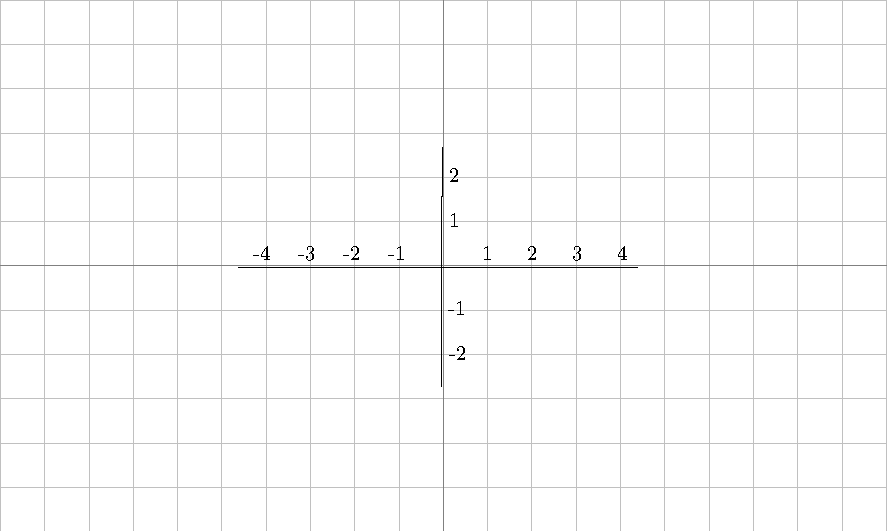
\includegraphics[scale=.9,bb = 115 65 310 190, clip=true]{II_1_3b-1.eps}
  
  %\vspace{0.5in}
  
  The plane is divided into four \textit{quadrants}, or sections, by a horizontal number line
  ($x$-axis) and a vertical number line ($y$-axis). The quadrants are numbered using the roman numerals I, II, III, and IV, beginning with the top-right quadrant (where both $x$ and $y$ are positive) and moving counter-clockwise.
\end{multicols}

 Where the two lines, or axes, meet
  in the center is called the origin. This center origin is where $x$ = 0 and $y$ = 0.\pp
	As we move to the right the numbers count up from zero,
  representing $x = 1, 2, 3 \ldots$. To the left the numbers count down from zero, representing \mbox{$x = - 1, - 2, - 3,\ldots$}.
 Similarly, as we move up the numbers count up from zero, \mbox{$y = 1, 2, 3,\ldots$}, and as we move down count down from zero, \mbox{$y = - 1, - 2, - 3\ldots$}.\pp
We can put dots on the graph which we will call points. Each point has an
``address'' that defines its location. The first number will be the value on
the $x - \tmop{axis}$ or horizontal number line. This is the distance the
point moves left/right from the origin. The second number will represent the
value on the $y - \tmop{axis}$ or vertical number line. This is the distance
the point moves up/down from the origin. The points are given as an ordered
pair $(x, y) .$\pp

 {\tmstrong{World View Note: }}Locations on the globe are given in the same
manner, each number is a distance from a central point, the origin which is
where the prime meridian and the equator. This ``origin is just off the
western coast of Africa.\pp

 The following example finds the address or coordinate pair for each of
several points on the coordinate plane.

\begin{example} \label{Lin42}
 Give the coordinates of each point.
  
  \begin{multicols}{2}
    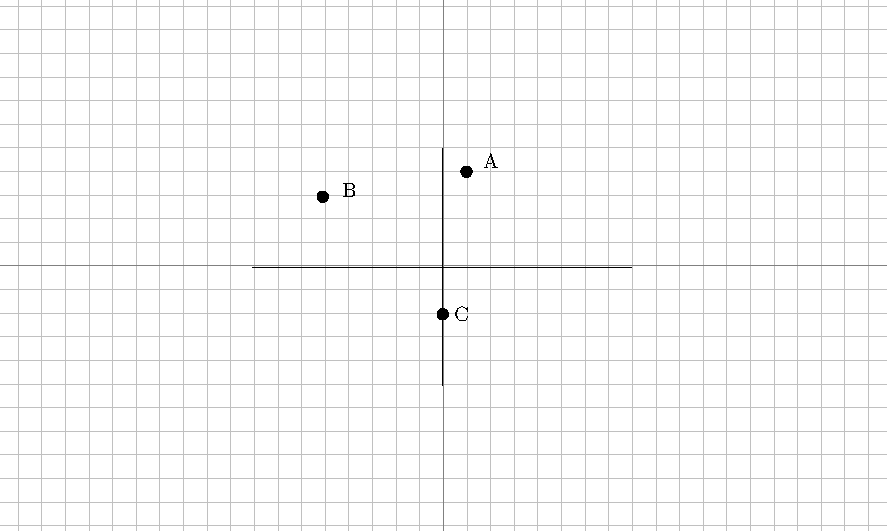
\includegraphics[scale=.9,bb = 115 65 310 190, clip=true]{II_1_3b-2.eps}
    
     Tracing from the origin, point A is right 1, up 4. This becomes A$(1, 4)$.
    Point B is left 5, up 3. Left is backwards or negative so we have B$(- 5,
    3)$. C is straight down 2 units. There is no left or right. This means we
    go right zero so the point is C$(0, - 2)$.
  \end{multicols}
  \begin{eqnarray*}
    A (1, 4), B (- 5, 3), C (0, - 2) &  & \tmop{Our} \tmop{solution}
  \end{eqnarray*}
\end{example}

 Just as we can give the coordinates for a set of points, we can take a set of
points and plot them on the plane.

\begin{example}\label{Lin43}
   Graph the points $A (3, 2), B (- 2, 1), C (3, - 4), D (- 2, - 3),$\\ $E (- 3,
  0), F (0, 2), G (0, 0)$
  
  \begin{multicols}{2}
    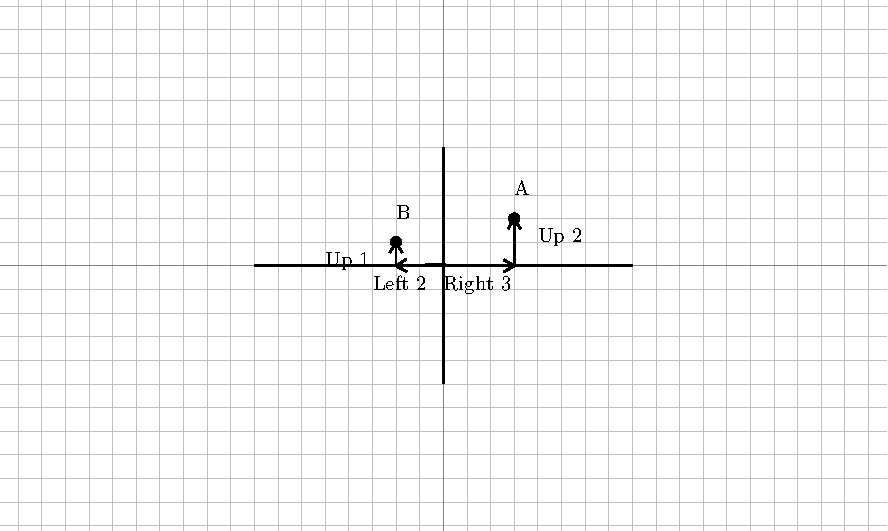
\includegraphics[scale=.9,bb = 115 65 310 190, clip=true]{II_1_3b-3.eps}
    
     The first point, A is at $(3, 2)$ this means $x = 3$ (right 3) and $y = 2$
    (up 2). Following these instructions, starting from the origin, we get our
    point.
    
    \
    
     The second point, $B (- 2, 1)$, is left 2 (negative moves backwards), up
    1. This is also illustrated on the graph. 
  \end{multicols}
  
  \
  
  \begin{multicols}{2}
    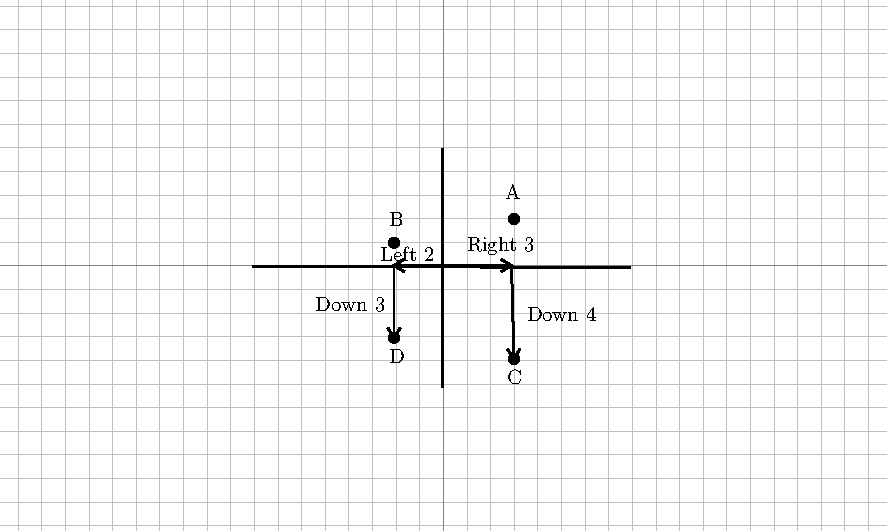
\includegraphics[scale=.9,bb = 115 65 310 190, clip=true]{II_1_3b-4.eps}
    
     The third point, $C (3, - 4)$ is right 3, down 4 (negative moves
    backwards).
    
    \
    
     The fourth point, D ($- 2, - 3$) is left 2, down 3 (both negative, both
    move backwards)
  \end{multicols}
  
   The last three points have zeros in them. We still treat these points just
  like the other points. If there is a zero there is just no movement.
  
  \begin{multicols}{2}
    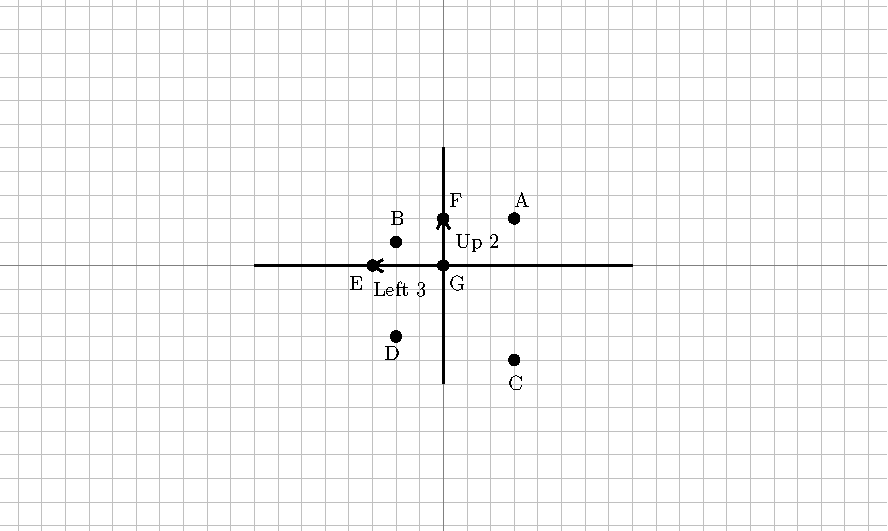
\includegraphics[scale=.9,bb = 115 65 310 190, clip=true]{II_1_3b-5.eps}
    
     Next is $E (- 3, 0)$. This is left 3 (negative is backwards), and up zero,
    right on the $x - \tmop{axis}$.
    
     Then is $F (0, 2)$. This is right zero, and up two, right on the $y -
    \tmop{axis}$.
    
     Finally is $G (0, 0)$. This point has no movement. Thus the point is right
    on the origin.
  \end{multicols}
  
  \
  
  \begin{multicols}{2}
    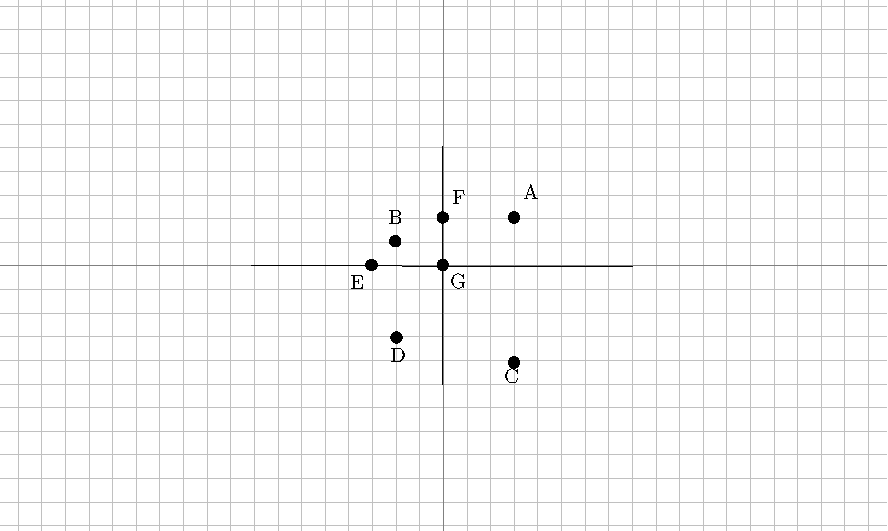
\includegraphics[scale=.9,bb = 115 65 310 190, clip=true]{II_1_3b-6.eps}
    
    \
    
    \
    
     Our solution
  \end{multicols}
\end{example}
\newpage
\subsection{Graphing Lines from Points}\pp

 {\tmstrong{Objective: Graph lines using $xy$-coordinates.}}\pp

 The main purpose of graphs is not to plot random points, but rather to give a
picture of the solutions to an equation. We may have an equation such as $y =
2 x - 3$. We may be interested in what type of solution are possible in this
equation. We can visualize the solution by making a graph of possible $x
\tmop{and} y$ combinations that make this equation a true statement. We will
have to start by finding possible $x \tmop{and} y$ combinations. We will do
this using a table of values.

\begin{example}\label{Lin44}
  \begin{eqnarray*}
    \tmop{Graph} y = 2 x - 3 &  & \tmop{We} \tmop{make~a} \tmop{table}
    \tmop{of} \tmop{values}\\
    &  & \\
    \begin{array}{|c|c|}
      \hline
      x & ~~y~~\\
      \hline
      - 1 & \\
      \hline
      0 & \\
      \hline
      1 & \\
      \hline
    \end{array} &  & \tmop{We} \tmop{will} \tmop{test} \tmop{three}
    \tmop{values} \tmop{for} x. \tmop{Any} \tmop{three} \tmop{can} \tmop{be}
    \tmop{used}\\
    &  & \\
    \begin{array}{|c|c|}
      \hline
      x & y\\
      \hline
      - 1 & - 5\\
      \hline
      0 & - 3\\
      \hline
      1 & - 1\\
      \hline
    \end{array} &  & \begin{array}{l}
      \tmop{Evaluate} \tmop{each} \tmop{by} \tmop{replacing} x \tmop{with}
      \tmop{the} \tmop{given} \tmop{value}\\
      x = - 1 ~~~~~~~ y = 2 (- 1) - 3 = - 2 - 3 = - 5\\
      x = 0  ~~~~~~~~~y = 2 (0) - 3 = 0 - 3 = - 3\\
      x = 1  ~~~~~~~~~y = 2 (1) - 3 = 2 - 3 = - 1
    \end{array}\\
    &  & \\
    (- 1, - 5), (0, - 3), (1, - 1) &  & \tmop{These} \tmop{then} \tmop{become}
    \tmop{the} \tmop{points} \tmop{to} \tmop{graph} \tmop{on} \tmop{our}
    \tmop{equation}
  \end{eqnarray*}
  \begin{multicols}{2}
    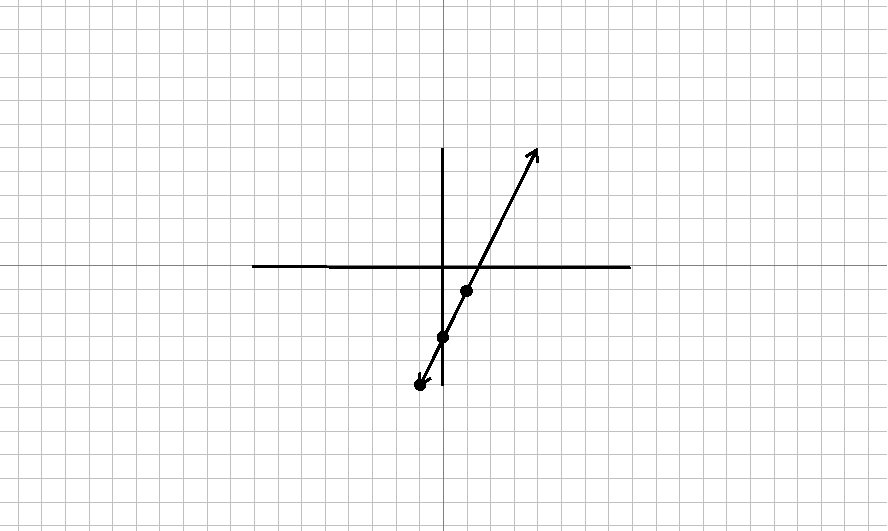
\includegraphics[scale=.9,bb = 115 65 310 190, clip=true]{II_1_3b-7.eps}
    
    \
    
     Plot each point.\\
    
     Once the point are on the graph, connect the dots to make a line.\\
    
     The graph is our solution.
  \end{multicols}
\end{example}

 What this line tells us is that any point on the line will work in the
equation $y = 2 x - 3$. For example, notice the graph also goes through the
point $(2, 1)$. If we use $x = 2$, we should get $y = 1$. Sure enough, $y = 2
(2) - 3 = 4 - 3 = 1$, just as the graph suggests. Thus we have the line is a
picture of all the solutions for $y = 2 x - 3$. We can use this table of
values method to draw a graph of any linear equation.

\begin{example}\label{Lin45}
  
  \begin{eqnarray*}
    \tmop{Graph} 2 x - 3 y = 6 &  & \tmop{We} \tmop{will} \tmop{use} \tmop{a}
    \tmop{table} \tmop{of} \tmop{values}\\
    &  & \\
    \begin{array}{|c|c|}
      \hline
      x & ~y~~\\
      \hline
      - 3 & \\
      \hline
      0 & \\
      \hline
      3 & \\
      \hline
    \end{array} &  & \tmop{We} \tmop{will} \tmop{test} \tmop{three}
    \tmop{values} \tmop{for} x. \tmop{~Any} \tmop{three} \tmop{can} \tmop{be}
    \tmop{used}.\\
    %&  & \\
      \end{eqnarray*}
      \begin{eqnarray*}
		2 (- 3) - 3 y = 6~ &  & \tmop{Substitute} \tmop{each} \tmop{value}
    \tmop{in} \tmop{for} x \tmop{and} \tmop{solve} \tmop{for} y\\
    - 6 - 3 y = 6~ &  & \tmop{Start} \tmop{with} x = - 3, \tmop{multiply}
    \tmop{first}\\
    \bf{\underline{+ 6 ~~~~~~~+ 6}} &  & \tmop{Add} 6 \tmop{to} \tmop{both} \tmop{sides}\\
    - 3 y = 12~ &  & \tmop{Divide} \tmop{both} \tmop{sides} \tmop{by} - 3\\
    \bf{\overline{- 3} ~~~ \overline{- 3}}~ &  & \\
    y = - 4~ &  & \tmop{solution} \tmop{for} y \tmop{when} x = - 3, \tmop{add}
    \tmop{this} \tmop{to} \tmop{table}\\
    &  & \\
    2 (0) - 3 y = 6~ &  & \tmop{Next} x = 0\\
    - 3 y = 6~ &  & \tmop{Multiplying} \tmop{clears} \tmop{the} \tmop{constant}
    \tmop{term}\\
    \bf{\overline{- 3} ~~~~ \overline{- 3}} &  & \tmop{Divide} \tmop{each} \tmop{side}
    \tmop{by} - 3\\
    y = - 2~ &  & \tmop{solution} \tmop{for} y \tmop{when} x = 0, \tmop{add}
    \tmop{this} \tmop{to} \tmop{table}\\
    &  & \\
    2 (3) - 3 y = 6~ &  & \tmop{Next} x = 3\\
    6 - 3 y = 6~ &  & \tmop{Multiply}\\
    \bf{\underline{- 6 ~~~~~~~~- 6}} &  & \tmop{Subtract} 9 \tmop{from} \tmop{both}
    \tmop{sides}\\
    - 3 y = 0~ &  & \tmop{Divide} \tmop{each} \tmop{side} \tmop{by} - 3\\
    \bf{\overline{- 3} ~~~ \overline{- 3}} &  & \\
    y = 0~ &  & \tmop{solution} \tmop{for} y \tmop{when} x = - 3, \tmop{add}
    \tmop{this} \tmop{to} \tmop{table}\\
    &  & \\
      \end{eqnarray*}
      \begin{eqnarray*}
		\begin{array}{|c|c|}
      \hline
      x & y\\
      \hline
      - 3 & - 4\\
      \hline
      0 & - 2\\
      \hline
      3 & 0\\
      \hline
    \end{array} &  & \tmop{Our} \tmop{completed} \tmop{table}\\
    &  & \\
    (- 3, - 4), (0, 2), (3, 0) &  & \tmop{Coordinate} \tmop{points} \tmop{from}
    \tmop{table}
  \end{eqnarray*}
  \begin{multicols}{2}
    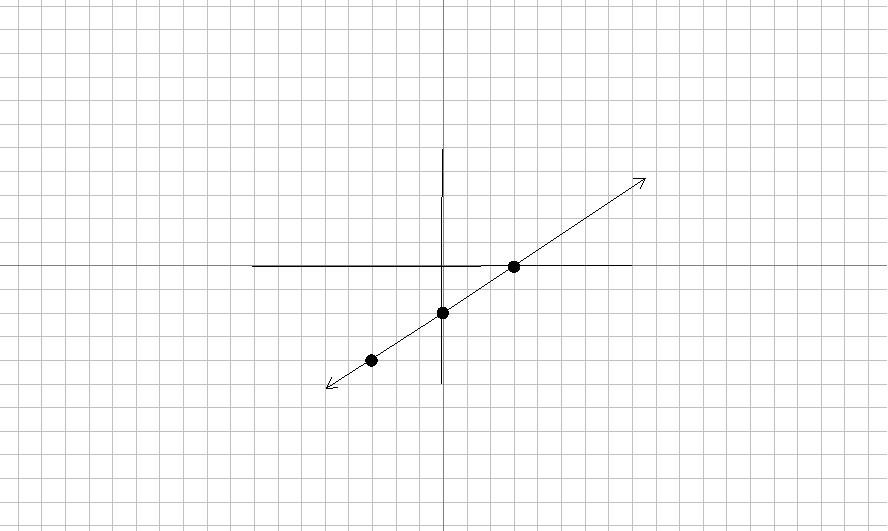
\includegraphics[scale=.9,bb = 115 65 310 190, clip=true]{II_1_3b-8.eps}
    
    \
    
     Graph points and connect dots
    
    \
    
     Our solution
  \end{multicols}
\end{example}
\newpage
\subsection{The Slope of a Line}\pp

 {\tmstrong{Objective: Find the slope of a line given a graph or two points.}}\pp

 As we graph lines, we will want to be able to identify different properties of
the lines we graph. One of the most important properties of a line is its
slope. {\tmstrong{Slope}} is a measure of steepness. A line with a large
slope, such as 25, is very steep. A line with a small slope, such as
$\frac{1}{10}$ is very flat. We will also use slope to describe the direction
of the line. A line that goes up from left to right will have a positive slope
and a line that goes down from left to right will have a negative slope.\pp

 As we measure steepness we are interested in how fast the line rises compared
to how far the line runs. For this reason we will describe slope as the
fraction $\frac{\tmop{rise}}{\tmop{run}}$. Rise would be a vertical change, or
a change in the $y$-values. Run would be a horizontal change, or a change in
the $x$-values. So another way to describe slope would be the fraction
$\frac{\tmop{change} \tmop{in} y}{\tmop{change} \tmop{in} x}$. It turns out
that if we have a graph we can draw vertical and horiztonal lines from one
point to another to make what is called a slope triangle. The sides of the
slope triangle give us our slope. The following examples show graphs that we
find the slope of using this idea.

\begin{example}\label{Lin46}
~\end{example}  
  \begin{multicols}{2}
    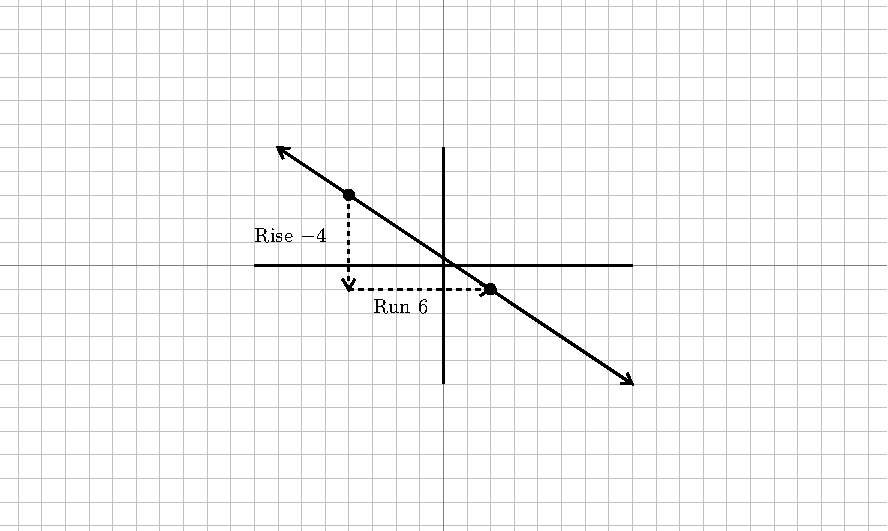
\includegraphics[scale=.9,bb = 115 65 310 190, clip=true]{II_1_3c-1.eps}
    
    \
    
    To find the slope of this line we will consider the rise, or vertical
    change and the run or horizontal change. Drawing these lines in makes a
    slope triangle that we can use to count from one point to the next the
    graph goes down 4, right 6. This is rise $- 4$, run 6. As a fraction it
    would be, $\frac{- 4}{6}$. Reduce the fraction to get $\frac{-2}{3}$.
  \end{multicols}
\begin{center}
A slope of $-\displaystyle\frac{2}{3}$ is our solution.
\end{center}%\end{example}
~\par
 {\tmstrong{World View Note: }}When French mathematicians Rene Descartes and
Pierre de Fermat first developed the coordinate plane and the idea of graphing
lines (and other functions) the $y$-axis was not a vertical line!\pp

\begin{example}\label{Lin47}
~\end{example}  
 \begin{multicols}{2}
    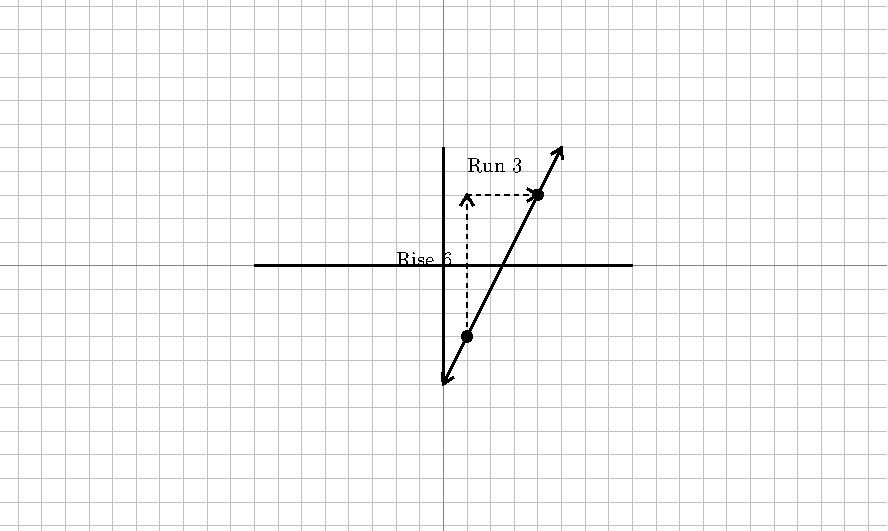
\includegraphics[scale=.9,bb = 115 65 310 190, clip=true]{II_1_3c-2.eps}
    
    To find the slope of this line, the rise is up 6, the run is right 3.\pp
		Our slope is then written as a fraction, $\frac{\tmop{rise}}{\tmop{run}}$ or
    $\frac{6}{3}$.\pp
		This fraction reduces to 2.  This will be our slope.
		  \end{multicols}
  %\begin{eqnarray*}
\begin{center}
A slope of $2$ is our solution.
\end{center}
  %\end{eqnarray*}
%\end{example}

 There are two special lines that have unique slopes that we need to be aware
of. They are illustrated in the following example.

\begin{example}\label{Lin48}
~\end{example}
  \begin{multicols}{2}
    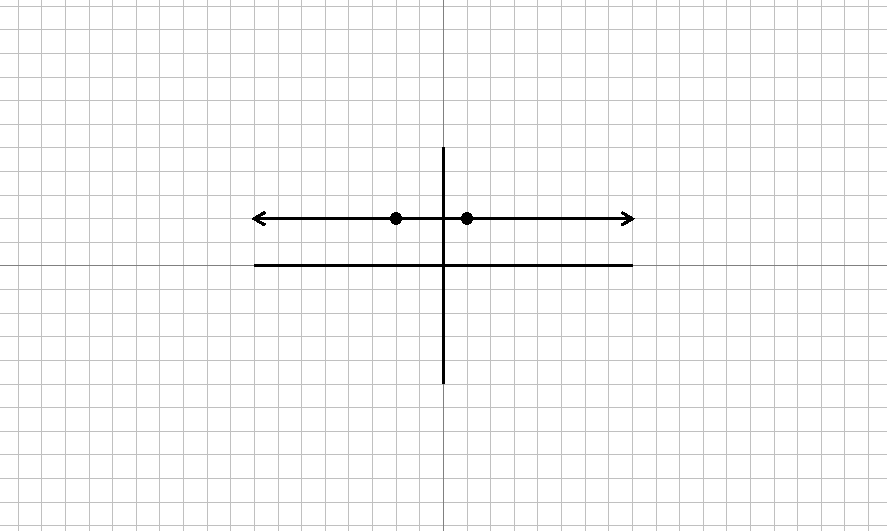
\includegraphics[scale=.9,bb = 115 65 310 190, clip=true]{II_1_3c-3.eps}
    
    In this graph there is no rise, but the run is 3 units. This slope becomes
    
    $\frac{0}{3} = 0$. \tmop{This} \tmop{line}, \tmop{and} \tmop{all}
    \tmop{horizontal} \tmop{lines} \tmop{have} a \tmop{zero} \tmop{slope}.
    
%    \ $
    
    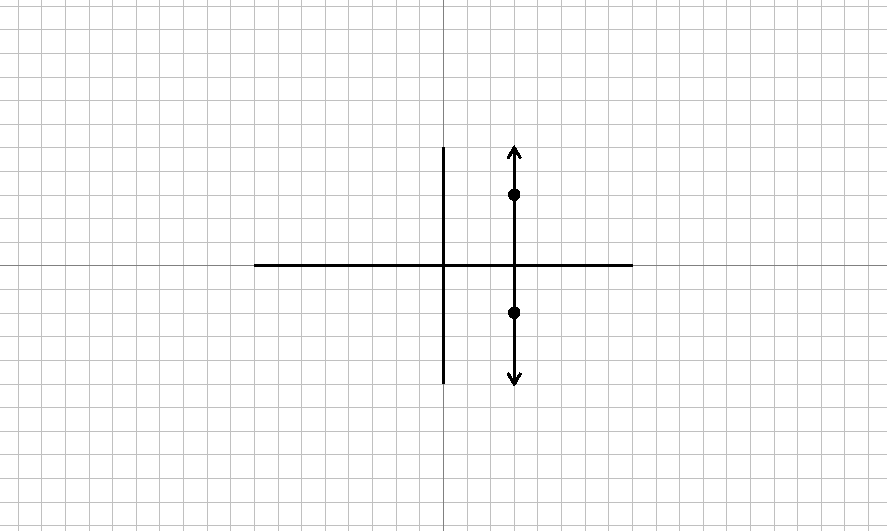
\includegraphics[scale=.9,bb = 115 65 310 190, clip=true]{II_1_3c-4.eps}
    
    This line has a rise of 5, but no run. The slope becomes $\frac{5}{0} =$
    \tmop{undefined}. \tmop{This} \tmop{line}, \tmop{and} \tmop{all}
    \tmop{vertical} \tmop{lines}, \tmop{have} \tmop{no} \tmop{slope}.
  \end{multicols}
%\end{example}

 As you can see there is a big difference between having a zero slope and
having no slope or undefined slope. Remember, slope is a measure of steepness.
The first slope is not steep at all, in fact it is flat. Therefore it has a
zero slope. The second slope can't get any steeper. It is so steep that there
is no number large enough to express how steep it is. This is an undefined
slope.\pp

 We can find the slope of a line through two points without seeing the points
on a graph. We can do this using a slope formula. If the rise is the change in
$y$ values, we can calculate this by subtracting the $y$ values of a point.
Similarly, if run is a change in the $x$ values, we can calculate this by
subtracting the $x$ values of a point. In this way we get the following
equation for slope.\pp

%\bbm
{\tmstrong{
\[ \tmop{The} \tmop{slope} \tmop{of} \tmop{a} \tmop{line} \tmop{through~} (x_1, y_1)
   \tmop{~and~} (x_2, y_2) \tmop{~is~} \frac{y_2 - y_1}{x_2 - x_1}. \]}}
%\ebm

 When mathematicians began working with slope, it was called the modular slope.
For this reason we often represent the slope with the variable $m$. Now we
have the following for slope.\pp

\bbm
\[ \tmmathbf{\tmop{Slope} = m = \frac{\tmop{rise}}{\tmop{run}} =
   \frac{\tmop{change} \tmop{in} y}{\tmop{change} \tmop{in} x} = \frac{y_2 -
   y_1}{x_2 - x_1}} \]
\ebm 
\pp
As we subtract the $y$ values and the $x$ values when calculating slope it is
important we subtract them in the same order. This process is shown in the
following examples.

\begin{example}\label{Lin49}
  
  \begin{eqnarray*}
    \tmop{Find} \tmop{the} \tmop{slope} \tmop{between} (- 4, 3) \tmop{~and~} (2,
    - 9) &  & \tmop{Identify} x_1, y_1, x_2, y_2\\
    (x_1, y_1) \tmop{~and~} (x_2, y_2) &  & \tmop{Use} \tmop{slope}
    \tmop{formula}, m = \frac{y_2 - y_1}{x_2 - x_1}\\
    m = \frac{- 9 - 3}{2 - (- 4)} &  & \tmop{Simplify}\\
    m = \frac{-12}{6} &  & \tmop{Reduce}\\
    m = - 2 &  & \tmop{Our} \tmop{solution}
  \end{eqnarray*}
\end{example}

\begin{example}\label{Lin50}
  \begin{eqnarray*}
    \tmop{Find} \tmop{the} \tmop{slope} \tmop{between} (4, 6) \tmop{~and~} (2, -
    1) &  & \tmop{Identify} x_1, y_1, x_2, y_2\\
    (x_1, y_1) \tmop{~and~} (x_2, y_2) &  & \tmop{Use} \tmop{slope}
    \tmop{formula}, m = \frac{y_2 - y_1}{x_2 - x_1}\\
    m = \frac{- 1 - 6}{2 - 4} &  & \tmop{Simplify}\\
    m = \frac{- 7}{- 2} &  & \tmop{Reduce}, \tmop{dividing} \tmop{by} - 1\\
    m = \frac{7}{2} &  & \tmop{Our} \tmop{solution}
  \end{eqnarray*}
\end{example}

 We may come up against a problem that has a zero slope (horizontal line) or no
slope (vertical line) just as with using the graphs.

\begin{example}\label{Lin51}
  
  \begin{eqnarray*}
    \tmop{Find} \tmop{the} \tmop{slope} \tmop{between~} (- 4, - 1) \tmop{~and~}
    (- 4, - 5) &  & \tmop{Identify} x_1, y_1, x_2, y_2\\
    (x_1, y_1) \tmop{~and~} (x_2, y_2) &  & \tmop{Use} \tmop{slope}
    \tmop{formula}, m = \frac{y_2 - y_1}{x_2 - x_1}\\
    m = \frac{- 5 - (- 1)}{- 4 - (- 4)} &  & \tmop{Simplify}\\
    m = \frac{- 4}{0} &  & \tmop{Can' t} \tmop{divide} \tmop{by} \tmop{zero}\\
    \tmop{Slope} m \tmop{is~undefined} &  & \tmop{Our} \tmop{solution}
  \end{eqnarray*}
\end{example}

\begin{example}\label{Lin52}
  \begin{eqnarray*}
    \tmop{Find} \tmop{the} \tmop{slope} \tmop{between~} (3, 1) \tmop{~and~} (- 2,
    1) &  & \tmop{Identify} x_1, y_1, x_2, y_2\\
    (x_1, y_1) \tmop{~and~} (x_2, y_2) &  & \tmop{Use} \tmop{slope}
    \tmop{formula}, m = \frac{y_2 - y_1}{x_2 - x_1}\\
    m = \frac{1 - 1}{- 2 - 3} &  & \tmop{Simplify}\\
    m = \frac{0}{- 5} &  & \tmop{Reduce}\\
    m = 0 &  & \tmop{Our} \tmop{solution}
  \end{eqnarray*}
\end{example}

 Again, there is a big difference between no slope and a zero slope. Zero is an
integer and it has a value, the slope of a flat horizontal line. No slope has
no value, it is undefined, the slope of a vertical line.\pp

 Using the slope formula we can also find missing points if we know what the
slope is. This is shown in the following two examples.

\pagebreak

\begin{example}\label{Lin53}~~
%~\pp
 Find the value of $y$ between the points (2, $y$) \tmop{~and~} \\(5, - 1) with
  slope $- 3$.\\
  \begin{eqnarray*}
    m = \frac{y_2 - y_1}{x_2 - x_1} &  & \tmop{We} \tmop{will} \tmop{plug}
    \tmop{values} \tmop{into~the} \tmop{slope} \tmop{formula}\\
    - 3 = \frac{- 1 - y}{5 - 2} &  & \tmop{Simplify}\\
    - 3 = \frac{- 1 - y}{3} &  & \tmop{Multiply} \tmop{both} \tmop{sides}
    \tmop{by} 3\\
    - 3 {\bf(3)} = \frac{- 1 - y}{3} {\bf(3)} &  & \tmop{Simplify}\\
    - 9 = - 1 - y &  & \tmop{Add} 1 \tmop{to} \tmop{both} \tmop{sides}\\
    \bf{\underline{+ 1 ~~~+ 1}}~~~~  &  & \\
    - 8 = - y &  & \tmop{Divide} \tmop{both} \tmop{sides} \tmop{by} - 1\\
    \bf{\overline{- 1} ~~~~ \overline{- 1}} &  & \\
    8 = y &  & \tmop{Our} \tmop{solution}
  \end{eqnarray*}
\end{example}

%\pagebreak

\begin{example}\label{Lin54}~~
%~\pp 
Find the value of $x$ between the points (- 3, 2) \tmop{~and~} \\($x$, 6) with
  slope $\displaystyle\frac{2}{5}$.\\
  \begin{eqnarray*}
    m = \frac{y_2 - y_1}{x_2 - x_1} &  & \tmop{We} \tmop{will} \tmop{plug}
    \tmop{values} \tmop{into} \tmop{slope} \tmop{formula}\\
    \frac{2}{5} = \frac{6 - 2}{x - (- 3)} &  & \tmop{Simplify}\\
    \frac{2}{5} = \frac{4}{x + 3} &  & \tmop{Multiply} \tmop{both}
    \tmop{sides} \tmop{by~} (x + 3) \\
    \frac{2}{5} (x + 3) = 4 &  & \tmop{Multiply} \tmop{by} 5 \tmop{to}
    \tmop{clear} \tmop{fraction}\\
    {\bf(5)} \frac{2}{5} (x + 3) = 4 {\bf(5)} &  & \tmop{Simplify}\\
    2 (x + 3) = 20 &  & \tmop{Distribute}\\
    2 x + 6 = 20 &  &  \\
    \bf{\underline{- 6 ~~- 6}} &  & \tmop{Subtract} 6 \tmop{from} \tmop{both}
    \tmop{sides}\\
    2 x = 14 &  & \tmop{Divide} \tmop{each} \tmop{side} \tmop{by} 2\\
    \bf{\overline{2} ~~~~~ \overline{2}}~ &  & \\
    x = 7 &  & \tmop{Our} \tmop{solution}
  \end{eqnarray*}
\end{example}
\newpage

\section{The Two Forms of a Linear Equation}
\subsection{Slope-Intercept Form}\pp

 {\tmstrong{Objective: Give the equation of a line with a known slope and
$y$-intercept.}}\pp

 When graphing a line we found one method we could use is to make a table of
values. However, if we can identify some properties of the line, we may be
able to make a graph much quicker and easier. One such method is finding the
slope and the $y$-intercept of the equation. The slope can be represented by $m$
and the $y$-intercept, where it crosses the axis and $x = 0$, can be represented
by $(0, b)$ where $b$ is the value where the graph crosses the vertical
$y$-axis. Any other point on the line can be represented by $(x, y)$. Using this
information we will look at the slope formula and solve the formula for $y$.

\begin{example}\label{Lin55}
  \begin{eqnarray*}
    m,~ (0, b),~ (x, y) &  & \tmop{Use} \tmop{the} \tmop{slope} \tmop{formula}\\
    \frac{y - b}{x - 0} = m &  & \tmop{Simplify}\\
    \frac{y - b}{x} = m &  & \tmop{Multiply} \tmop{both} \tmop{sides}
    \tmop{by} x\\
    y - b = m x &  & \tmop{Add} b \tmop{to} \tmop{both} \tmop{sides}\\
    \tmmathbf{\underline{+ b ~~~+ b}} &  & \\
    y = m x + b &  & \tmop{Our} \tmop{solution}
  \end{eqnarray*}
\end{example}

 This equation, $y = m x + b$ can be thought of as the equation of any line
that as a slope of $m$ and a $y$-intercept of $b$. This formula is known as the
slope-intercept formula or equation.\pp

\bbm
 {\tmstrong{\[ \tmop{Slope} - \tmop{intercept~} \tmop{equation} : y = m x + b
\]}}
\ebm

~\par

 If we know the slope and the $y$-intercept we can easily find the equation that
represents the line.

\begin{example}\label{Lin56}
  \begin{eqnarray*}
    \tmop{Slope} = \frac{3}{4},~~ y - \tmop{intercept} = - 3 &  & \tmop{Use}
    \tmop{the} \tmop{slope} - \tmop{intercept} \tmop{equation}\\
    y = m x + b &  & m \tmop{is} \tmop{the} \tmop{slope},~~ b \tmop{is}
    \tmop{the} y - \tmop{intercept}\\
    y = \frac{3}{4} x - 3 &  & \tmop{Our} \tmop{solution}
  \end{eqnarray*}
\end{example}

 We can also find the equation by looking at a graph and finding the slope and
$y$-intercept.

\begin{example}\label{Lin57}
~\end{example}

  \begin{multicols}{2}
    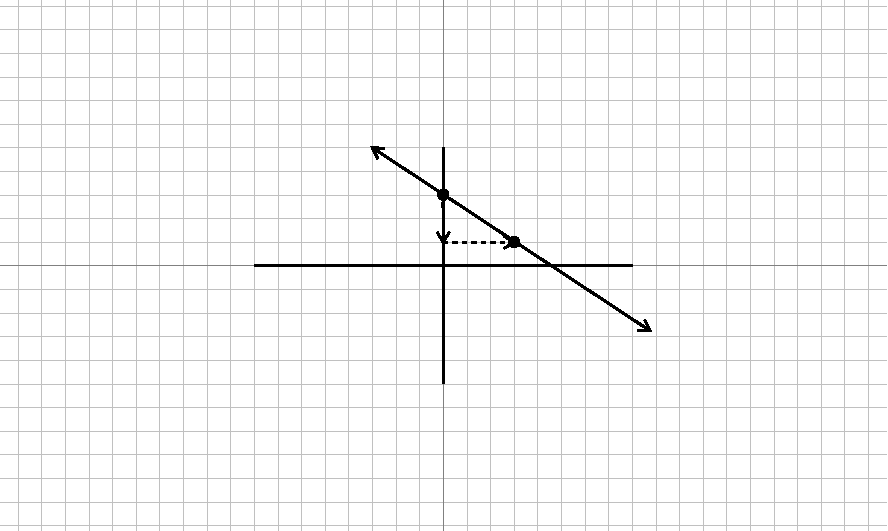
\includegraphics[scale=.9,bb = 115 65 310 190, clip=true]{II_1_4a-1.eps}
    
 Identify the point where the graph crosses the $y$-axis (0,3).\\ This means the $y$-intercept is 3.\pp
    
 Identify one other point and draw a slope triangle to find the slope.\pp
The slope is $m=- \frac{2}{3}$.
  \end{multicols}

\begin{center}
  $y = m x + b\qquad\qquad\qquad$ Slope-intercept equation\\
  $y = - \frac{2}{3} x + 3\qquad\qquad\qquad$ Our solution\qquad\qquad~~~
\end{center}

 % y = - \frac{2}{3} x + 3 &  & \tmop{Our} \tmop{solution}
%\end{eqnarray*}
%\end{example}

 We can also move the opposite direction, using the equation identify the slope
and $y$-intercept and graph the equation from this information. However, it will
be important for the equation to first be in slope intercept form. If it is
not, we will have to solve it for $y$ so we can identify the slope and the
$y$-intercept.

\begin{example}\label{Lin58}~~~Write the equation $2x=4y=6$ in slope-intercept form.
  
  \begin{eqnarray*}
    2 x - 4 y = 6~~ &  & \tmop{Solve} \tmop{for} y\\
    \tmmathbf{\underline{- 2 x ~~~~- 2 x}} &  & \tmop{Subtract} 2 x \tmop{from} \tmop{both}
    \tmop{sides}\\
    - 4 y = - 2 x + 6 &  & \tmop{Put} x \tmop{term} \tmop{first}\\
    \tmmathbf{\overline{- 4} ~~~~ \overline{- 4} ~~ \overline{- 4}} &  & \tmop{Divide~}
    \tmop{each} \tmop{term} \tmop{by} - 4\\
    y = \frac{1}{2} x - \frac{3}{2} &  & \tmop{Our} \tmop{solution}
  \end{eqnarray*}
\end{example}

 Once we have an equation in slope-intercept form we can graph it by first
plotting the $y$-intercept, then using the slope, finding a second point and
connecting the dots.

\begin{example}\label{Lin59}~~~Graph $y=\displaystyle\frac{1}{2}x-4$.
  \begin{eqnarray*}
    y = m x + b&  & \tmop{Slope} - \tmop{intercept} \tmop{equation}\\
    m = \frac{1}{2},~ b = - 4 &  & \tmop{Identify} \tmop{the} \tmop{slope},~ m, \tmop{and} \tmop{the} y - \tmop{intercept},~ b
  \end{eqnarray*}
  \begin{center}
	Now make the graph.
	\end{center}
	\begin{multicols}{2}~\par
    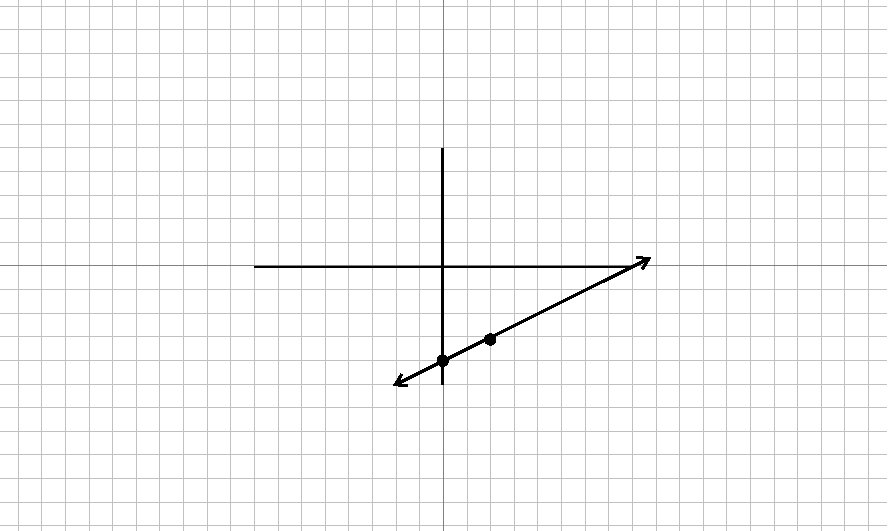
\includegraphics[scale=.9,bb = 115 65 310 190, clip=true]{II_1_4a-2.eps}
    
     Starting with a point at the \\
		$y$-intercept of $- 4$.\\
    
     Then use the slope $\frac{\tmop{rise}}{\tmop{run}}$, so we will rise 1
    unit and run 2 units to find the next point.\\
    
     Once we have both points, connect the dots to get our graph.
  \end{multicols}
\end{example}

\pp

 {\tmstrong{World View Note:}} Before our current system of graphing, French
Mathematician Nicole Oresme, in 1323 suggested graphing lines that would look
more like a bar graph with a constant slope!\pp

\begin{example}\label{Lin60}~~~Graph $3x+4y=12$.
  \begin{eqnarray*}
    3 x + 4 y = 12~~ &  & \tmop{Not} \tmop{in} \tmop{slope-intercept} \tmop{form}\\
    \tmmathbf{\underline{- 3 x ~~~~~~- 3 x}} &  & \tmop{Subtract} 3 x \tmop{from} \tmop{both}
    \tmop{sides}\\
    4 y = - 3 x + 12 &  & \tmop{Put} \tmop{the} x \tmop{term} \tmop{first}\\
    \tmmathbf{\overline{4} ~~~~~~~ \overline{4} ~~~~~ \overline{4}}~ &  & \tmop{Divide} \tmop{each}
    \tmop{term} \tmop{by} 4\\
    y = - \frac{3}{4} x + 3 &  & \tmop{Now~in} \tmop{slope} - \tmop{intercept}
    \tmop{form}\\
    m = - \frac{3}{4},~ b = 3 &  & \tmop{Identify} m \tmop{and} b
  \end{eqnarray*}
  \begin{center}
Now make the graph.
	\end{center}
\end{example}
  \begin{multicols}{2}
	~\par
    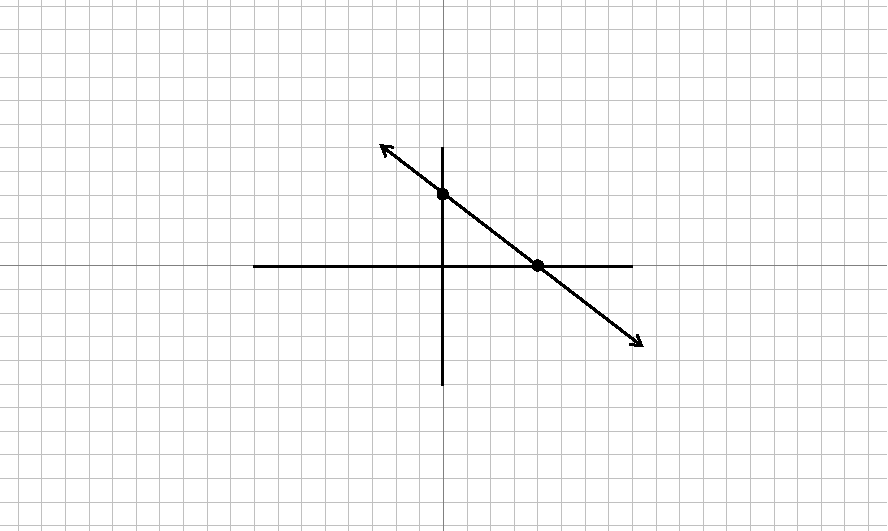
\includegraphics[scale=.9,bb = 115 65 310 190, clip=true]{II_1_4a-3.eps}
    
    \
    
     Starting with a point at the \\$y$-intercept of $3$.\\
    
 Then use the slope $\frac{\tmop{rise}}{\tmop{run}}$, but its negative so
    it will go downhill, so we will drop 3 units and run 4 units to find the
    next point.\\
    
     Once we have both points, connect the dots to get our graph.
  \end{multicols}

 We want to be very careful not to confuse using slope to find the next point
with use a coordinate such as $(4, - 2)$ to find an individual point.
Coordinates such as $(4, - 2)$ start from the origin and move horizontally
first, and vertically second. Slope starts from a point on the line that could
be anywhere on the graph. The numerator is the vertical change and the
denominator is the horizontal change.\pp

 Lines with zero slope or no slope can make a problem seem very different.  Such lines are horizontal.
A horizontal line will have a slope of zero which when
multiplied by $x$ gives zero. So the equation simply becomes $y = b$ or $y$ is
equal to the $y$-coordinate of the graph. If we have no slope, or a vertical
line, the equation can't be written in slope intercept at all because the
slope is undefined. There is no $y$ in these equations. We will simply make
$x$ equal to the $x$-coordinate of the graph.

\begin{example}\label{Lin61}
~\end{example}
  
  \begin{multicols}{2}
    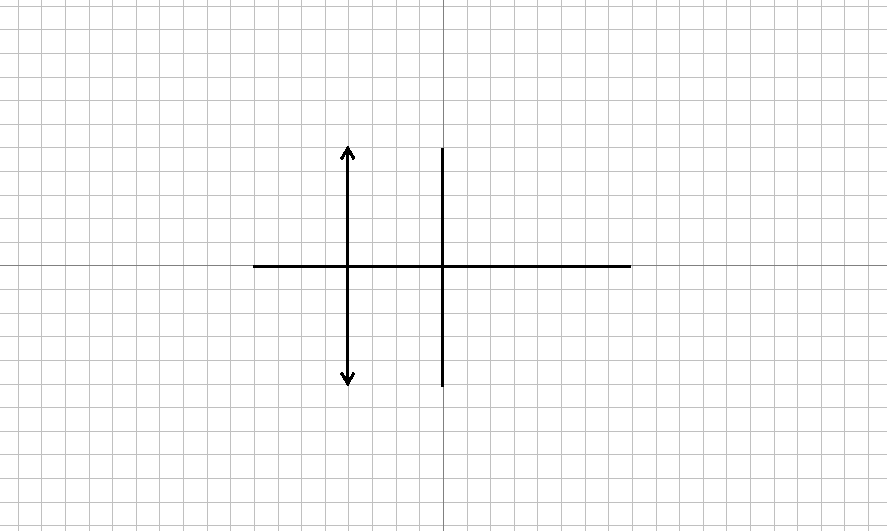
\includegraphics[scale=.9,bb = 115 65 310 190, clip=true]{II_1_4a-4.eps}
    
Give the equation of the line in the graph.\pp 
Because we have a vertical line and no slope there is no slope-intercept equation we can use.\pp
Rather we make $x$ equal to the $x$-coordinate of $- 4$
  \end{multicols}
	\begin{center}
	    Our solution is $x = - 4$.
	\end{center}
%\end{example}

\newpage
\subsection{Point-Slope Form}\pp

 {\tmstrong{Objective: Give the equation of a line with a known slope and
point.}}\pp

 The slope-intercept form has the advantage of being simple to remember and
use, however, it has one major disadvantage: we must know the $y$-intercept in
order to use it! Generally we do not know the y-intercept, we only know one or
more points (that are not the $y$-intercept). In these cases we can't use the
slope intercept equation, so we will use a different, more flexible formula. If
we let the slope of an equation be $m$, and a specific point on the line be
$(x_1, y_1)$, and any other point on the line be $(x, y)$. We can use the
slope formula to make a second equation.

\begin{example}\label{Lin62}
  
  \begin{eqnarray*}
    m,~ (x_1, y_1),~ (x, y) &  & \tmop{Recall} \tmop{slope} \tmop{formula}\\
    \frac{y_2 - y_1}{x_2 - x_1} = m &  & \tmop{Plug} \tmop{in} \tmop{values}\\
    \frac{y - y_1}{x - x_1} = m &  & \tmop{Multiply} \tmop{both} \tmop{sides}
    \tmop{by} (x - x_1)\\
    y - y_1 = m (x - x_1) &  & \tmop{Our} \tmop{equation}
  \end{eqnarray*}
\end{example}

 If we know the slope, $m$ of an equation and any point on the line $(x_1,
y_1)$ we can easily plug these values into the equation above which will be
called the point-slope formula or equation.\pp

\bbm
 {\tmstrong{\[ \tmop{Point} - \tmop{slope~} \tmop{equation} : y - y_1 = m (x -
   x_1) \]}}
\ebm
\pp

\begin{example}\label{Lin63}
 ~\pp
Write the equation of the line through the point $(3, - 4)$ with a slope of
  $\displaystyle\frac{3}{5}$.
  \begin{eqnarray*}
    y - y_1 = m (x - x_1) &  & \tmop{Plug} \tmop{values} \tmop{into}
    \tmop{point} - \tmop{slope} \tmop{formula}\\
    y - (- 4) = \frac{3}{5} (x - 3) &  & \tmop{Simplify} \tmop{signs}\\
    y + 4 = \frac{3}{5} (x - 3) &  & \tmop{Our} \tmop{solution}
  \end{eqnarray*}
\end{example}

 Often, we will prefer final answers be written in slope-intercept form. If the
directions ask for the answer in slope-intercept form we will simply
distribute the slope, then solve for $y$.

\begin{example}\label{Lin64}
~\pp
   Write the equation of the line through the point $(- 6, 2)$ with a slope of
  $- \displaystyle\frac{2}{3}$ in slope-intercept form.
  \begin{eqnarray*}
    y - y_1 = m (x - x_1) &  & \tmop{Plug} \tmop{values} \tmop{into}
    \tmop{point} - \tmop{slope} \tmop{formula}\\
    y - 2 = - \frac{2}{3} \left(x - (- 6)\right) &  & \tmop{Simplify} \tmop{signs}\\
    y - 2 = - \frac{2}{3} (x + 6) &  & \tmop{Distribute~} \tmop{slope}\\
    y - 2 = - \frac{2}{3} x - 4 &  & \tmop{Solve} \tmop{for} y \tmop{by~adding~2~to~both~sides}\\
    \tmmathbf{\underline{+ 2 ~~~~~~~~ + 2}} &  & \\
    y = - \frac{2}{3} x - 2 &  & \tmop{Our} \tmop{solution}
  \end{eqnarray*}
\end{example}

 An important thing to observe about the point slope formula is that the
operation between the $x$'s and $y$'s is subtraction. This means when you
simplify the signs you will have the opposite of the numbers in the point. We
need to be very careful with signs as we use the point-slope formula.\pp

 In order to find the equation of a line we will always need to know the slope.
If we don't know the slope to begin with we will have to do some work to find
it first before we can get an equation.

\begin{example}\label{Lin65}
~\pp
   Find the equation of the line through the points $(- 2, 5) \tmop{and} (4, -
  3)$.
  \begin{eqnarray*}
    m = \frac{y_2 - y_1}{x_2 - x_1} &  & \tmop{First} \tmop{we} \tmop{must}
    \tmop{find} \tmop{the} \tmop{slope}\\
    m = \frac{- 3 - 5}{4 - (- 2)} = \frac{- 8}{6} = - \frac{4}{3} &  &
    \tmop{Plug} \tmop{values} \tmop{in} \tmop{slope} \tmop{formula} \tmop{and}
    \tmop{evaluate}\\
    y - y_1 = m (x - x_1) &  & \tmop{Use} \tmop{point} - \tmop{slope}
    \tmop{formula},\\
		& & \tmop{~~~plugging~in~slope~and~either~point}\\
    y - 5 = - \frac{4}{3} (x - (- 2)) &  & \tmop{Simplify} \tmop{signs}\\
    y - 5 = - \frac{4}{3} (x + 2) &  & \tmop{Our} \tmop{solution}
  \end{eqnarray*}
\end{example}

\begin{example}\label{Lin66}
~\pp
   Find the equation of the line through the points $(- 3, 4) \tmop{and} (- 1,
  - 2)$ in slope-intercept form.
  \begin{eqnarray*}
    m = \frac{y_2 - y_1}{x_2 - x_1} &  & \tmop{First} \tmop{we} \tmop{must}
    \tmop{find} \tmop{the} \tmop{slope}\\
    m = \frac{- 2 - 4}{- 1 - (- 3)} = \frac{- 6}{2} = - 3 &  & \tmop{Plug}
    \tmop{values} \tmop{in} \tmop{slope} \tmop{formula} \tmop{and}
    \tmop{evaluate}\\
    y - y_1 = m (x - x_1) &  & \tmop{Use} \tmop{point} - \tmop{slope} \tmop{formula},\\
		& &  \tmop{~~~plugging~in~slope~and~either~point}\\
    y - 4 = - 3 (x - (- 3)) &  & \tmop{Simplify} \tmop{signs}\\
    y - 4 = - 3 (x + 3) &  & \tmop{Distribute~} \tmop{slope}\\
    y - 4 = - 3 x - 9 &  & \tmop{Solve} \tmop{for} y \\
    \tmmathbf{\underline{+ 4 ~~~~~~~~~+ 4}} &  & \tmop{Add} 4 \tmop{to} \tmop{both} \tmop{sides}\\
    y = - 3 x - 5 &  & \tmop{Our} \tmop{solution}
  \end{eqnarray*}
\end{example}

\begin{example}\label{Lin67}
~\pp
   Find the equation of the line through the points $(6, - 2)$ and $(- 4, 1)$
  in slope-intercept form.
  \begin{eqnarray*}
    m = \frac{y_2 - y_1}{x_2 - x_1} &  & \tmop{First} \tmop{we} \tmop{must}
    \tmop{find} \tmop{the} \tmop{slope}\\
    m = \frac{1 - (- 2)}{- 4 - 6} = \frac{3}{- 10} = - \frac{3}{10} &  &
    \tmop{Plug} \tmop{values} \tmop{into} \tmop{slope} \tmop{formula}
    \tmop{and} \tmop{evaluate}\\
    y - y_1 = m (x - x_1) &  & \tmop{Use} \tmop{point} - \tmop{slope}
    \tmop{formula},\\
		& &  \tmop{~~~plugging~in~slope~and~either~point}\\
    y - (- 2) = - \frac{3}{10} (x - 6) &  & \tmop{Simplify} \tmop{signs}\\
    y + 2 = - \frac{3}{10} (x - 6) &  & \tmop{Distribute} \tmop{slope~}\\
    y + 2 = - \frac{3}{10} x + \frac{9}{5} &  & \tmop{Solve} \tmop{for} y,
    \tmop{by~subtracting} 2 \tmop{from} \tmop{both} \tmop{sides}\\
    \tmmathbf{\underline{- 2 ~~~~~~~~~- \frac{10}{5}}} &  & \tmop{Use} \frac{10}{5} \tmop{on}
    \tmop{right} \tmop{so} \tmop{we} \tmop{have} \tmop{a} \tmop{common}
    \tmop{denominator}\\
    & & \\
		y = - \frac{3}{10} x - \frac{1}{5} &  & \tmop{Our} \tmop{solution}
  \end{eqnarray*}
\end{example}

 {\tmstrong{World View Note:}} The city of K$\ddot{\text{o}}$nigsberg (now Kaliningrad, Russia)
had a river that flowed through the city breaking it into several parts. There
were 7 bridges that connected the parts of the city. In 1735 Leonhard Euler
considered the question of whether it was possible to cross each bridge
exactly once and only once. It turned out that this problem was impossible,
but the work laid the foundation of what would become graph theory.

\newpage

\section{Parallel and Perpendicular Lines}

 {\tmstrong{Objective: Identify the equation of a line given a parallel or
perpendicular line.}}\pp

 There is an interesting connection between the slopes of lines that are
parallel, as well as the slopes of lines that are perpendicular (meet at a right
angle). This is shown in the following example.

\begin{example}\label{Lin68}
~\end{example}

  \begin{multicols}{2}
    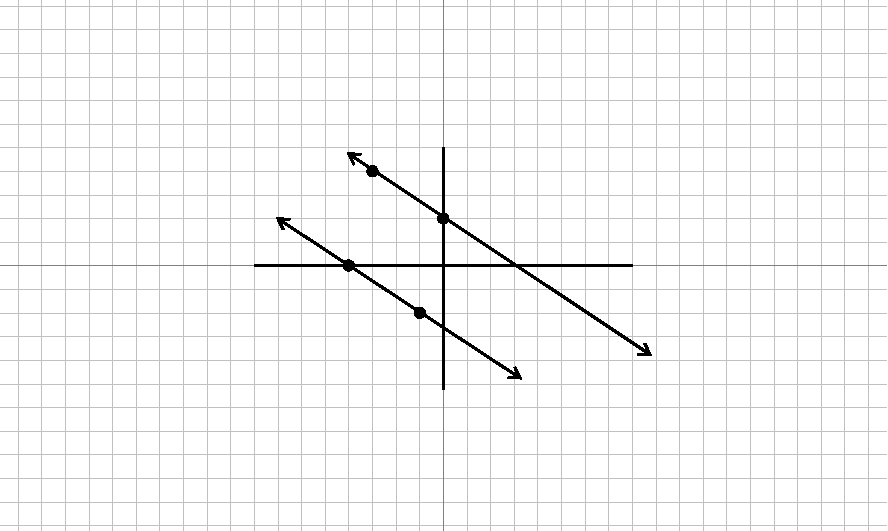
\includegraphics[scale=.9,bb = 115 65 310 190, clip=true]{II_1_5-1.eps}
    
     The above graph has two parallel lines. The slope of the top line is down
    2, run 3, or $- \frac{2}{3}$.\\
		The slope of the bottom line is down 2, run 3 as well, or $- \frac{2}{3}$.
    
    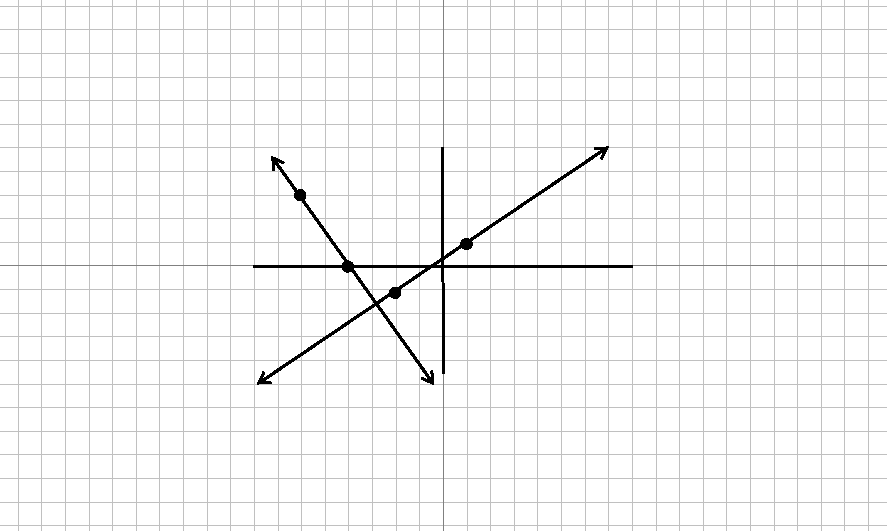
\includegraphics[scale=.9,bb = 115 65 310 190, clip=true]{II_1_5-2.eps}
    
     The above graph has two perpendicular lines. The slope of the flatter line
    is up 2, run 3 or $\frac{2}{3}$.\\
		The slope of the steeper line is down 3, run 2, or $- \frac{3}{2}$.
  \end{multicols}
%\end{example}
~\par

 As the first graph above illustrates, parallel lines have the same slope.\pp
On the other hand, perpendicular lines are said to have \textit{negative reciprocal} slopes.   More precisely, if two lines with slopes $m_1$ and $m_2$ are known to be perpendicular, then $m_2=-~\displaystyle\frac{1}{m_1}$ (and so, $m_1m_2=-1$).\pp
We can use these properties to make conclusions about parallel and perpendicular lines.\pp

{\tmstrong{World View Note:}} Greek Mathematician Euclid lived around 300 BC
and published a book titled, {\tmem{The Elements}}. In it is the famous
parallel postulate which mathematicians have tried for years to drop from the
list of postulates. The attempts have failed, yet all the work done has
developed new types of geometries!\pp

\begin{example}\label{Lin69}~~~Find the slope of a line parallel to $5 y - 2 x = 7$.
  \begin{eqnarray*}
    5 y - 2 x = 7~~~~~ &  & \tmop{To} \tmop{find} \tmop{the} \tmop{slope} \tmop{we}
    \tmop{will} \tmop{put} \tmop{equation} \tmop{in} \tmop{slope} -
    \tmop{intercept} \tmop{form}\\
    \tmmathbf{\underline{+ 2 x ~~ + 2 x}} &  & \tmop{Add} 2 x \tmop{to} \tmop{both}
    \tmop{sides}\\
    5 y = 2 x + 7~~~~~ &  & \tmop{Put} x \tmop{term} \tmop{first}\\
    \tmmathbf{\overline{5} ~~~~ \overline{5} ~~~~~ \overline{5}}~~~~~ &  & \tmop{Divide} \tmop{each}
    \tmop{term} \tmop{by} 5\\
    y = \frac{2}{5} x + \frac{7}{5}~~~~~ &  & \tmop{The} \tmop{slope} \tmop{is}
    \tmop{the} \tmop{coefficient} \tmop{of} x\\
    &  & \\
    m = \frac{2}{5}~~~~~ &  & \tmop{Slope} \tmop{of} \tmop{given} \tmop{line}\\
		& & \tmop{Parallel} \tmop{lines} \tmop{have} \tmop{the} \tmop{same}
    \tmop{slope}\\
    &  & \\
    m = \frac{2}{5}~~~~~ &  & \tmop{Our} \tmop{solution}
  \end{eqnarray*}
\end{example}

\begin{example}\label{Lin70}~~~Find the slope of a line perpendicular to $3 x - 4 y = 2$.
  \begin{eqnarray*}
    3 x - 4 y = 2~~~~ &  & \tmop{To} \tmop{find} \tmop{slope} \tmop{we}
    \tmop{will} \tmop{put} \tmop{equation} \tmop{in} \tmop{slope} -
    \tmop{intercept} \tmop{form}\\
    \tmmathbf{\underline{- 3 x ~~~~~~~~- 3 x}} &  & \tmop{Subtract} 3 x \tmop{from} \tmop{both}
    \tmop{sides}\\
    - 4 y = - 3 x + 2~~~~~ &  & \tmop{Put} x \tmop{term} \tmop{first}\\
    \tmmathbf{\overline{- 4} ~~~ \overline{- 4} ~~ \overline{- 4}}~~~~~ &  & \tmop{Divide}
    \tmop{each} \tmop{term} \tmop{by} - 4\\
    y = \frac{3}{4} x - \frac{1}{2}~~~~ &  & \tmop{The} \tmop{slope} \tmop{is}
    \tmop{the} \tmop{coefficient} \tmop{of} x\\
    &  & \\
    m = \frac{3}{4}~~~~ &  & \tmop{Slope} \tmop{of} \tmop{given} \tmop{line}\\
		& & \tmop{Perpendicular} \tmop{lines} \tmop{have} \tmop{negative}
    \tmop{reciprocal} \tmop{slopes}\\
    &  & \\
    m = - \frac{4}{3}~~~~ &  & \tmop{Our} \tmop{solution}
  \end{eqnarray*}
\end{example}

 Once we have a slope, it is possible to find the complete equation of the
desired line, if we know one point on it.

\pagebreak

\begin{example}\label{Lin71}~~~Find the equation of a line through $(4, - 5)$ and parallel to $2 x - 3 y =
  6$.
  \begin{eqnarray*}
    2 x - 3 y = 6~~~~ &  & \tmop{We} \tmop{first} \tmop{need} \tmop{slope}
    \tmop{of} \tmop{parallel} \tmop{line}\\
    \tmmathbf{\underline{- 2 x ~~~~~~~~- 2 x}} &  & \tmop{Subtract} 2 x \tmop{from} \tmop{each}
    \tmop{side}\\
    - 3 y = - 2 x + 6~~~~ &  & \tmop{Put} x \tmop{term} \tmop{first}\\
    \tmmathbf{\overline{- 3} ~~~~ \overline{- 3} ~~ \overline{- 3}}~~~ &  & \tmop{Divide}
    \tmop{each} \tmop{term} \tmop{by} - 3\\
    y = \frac{2}{3} x - 2~~~~ &  & \tmop{Identify} \tmop{the} \tmop{slope},
    \tmop{the} \tmop{coefficient} \tmop{of} x\\
    &  & \\
    m = \frac{2}{3}~~~~ &  & \tmop{Parallel} \tmop{lines} \tmop{have} \tmop{the}
    \tmop{same} \tmop{slope}\\
    &  & \\
    m = \frac{2}{3}~~~~ &  & \tmop{We} \tmop{will} \tmop{use} \tmop{this}
    \tmop{slope} \tmop{and} \tmop{our} \tmop{point} (4, - 5)\\
    &  & \\
    y - y_1 = m (x - x_1)~~~~ &  & \tmop{Plug} \tmop{this} \tmop{information}
    \tmop{into} \tmop{point}-\tmop{slope} \tmop{formula}\\
    y - (- 5) = \frac{2}{3} (x - 4)~~~~ &  & \tmop{Simplify} \tmop{signs}\\
    &  & \\
    y + 5 = \frac{2}{3} (x - 4)~~~~ &  & \tmop{Our} \tmop{solution}
  \end{eqnarray*}
\end{example}

\begin{example}\label{Lin72}~~~Find the equation of the line through $(6, - 9)$ perpendicular to $y = -
  \displaystyle\frac{3}{5} x + 4$ in slope-intercept form.
\end{example}
  \begin{eqnarray*}
    y = - \frac{3}{5} x + 4 &  & \tmop{Identify} \tmop{the} \tmop{slope},
    \tmop{coefficient} \tmop{of} x\\
    &  & \\
    m = - \frac{3}{5} &  & \tmop{Perpendicular} \tmop{lines} \tmop{have}
    \tmop{negative} \tmop{reciprocal} \tmop{slopes}\\
    &  & \\
    m = \frac{5}{3} &  & \tmop{We} \tmop{will} \tmop{use} \tmop{this}
    \tmop{slope} \tmop{and} \tmop{our} \tmop{point} (6, - 9) \\
    &  & \\
    y - y_1 = m (x - x_1) &  & \tmop{Plug} \tmop{this} \tmop{information}
    \tmop{into} \tmop{point} - \tmop{slope} \tmop{formula}\\
    &  & \\
    y - (- 9) = \frac{5}{3} (x - 6) &  & \tmop{Simplify} \tmop{signs}\\
    &  & \\
    y + 9 = \frac{5}{3} (x - 6) &  & \tmop{Distribute} \tmop{slope}
  \end{eqnarray*}
  \begin{eqnarray*}
  %  &  & \\
    y + 9 = \frac{5}{3} x - 10 &  & \tmop{Solve} \tmop{for} y\\
    \tmmathbf{\underline{- 9 ~~~~~~~~- 9}} &  & \tmop{Subtract} 9 \tmop{from} \tmop{both}
    \tmop{sides}\\
    y = \frac{5}{3} x - 19 &  & \tmop{Our} \tmop{solution}
  \end{eqnarray*}

 Zero slopes and undefined slopes may seem like opposites (one is a horizontal line,
one is a vertical line). Because a horizontal line is perpendicular to a
vertical line we can say that an undefined slope and a zero slope are actually
perpendicular slopes!

\begin{example}\label{Lin73}~~~Find the equation of the line through (3, 4) perpendicular to $x = - 2$.
  \begin{eqnarray*}
    x = - 2~~ &  & \tmop{This} \tmop{equation} \tmop{has} \tmop{an~undefined}
    \tmop{slope}, \tmop{a~vertical} \tmop{line}\\
    \tmop{Undefined} \tmop{slope}~~ &  & \tmop{Perpendicular} \tmop{line} \tmop{then}
    \tmop{would} \tmop{have} \tmop{a~zero} \tmop{slope}\\
    m = 0~~ &  & \tmop{Use} \tmop{this} \tmop{and} \tmop{our} \tmop{point} (3,
    4)\\
    y - y_1 = m (x - x_1)~~ &  & \tmop{Plug} \tmop{this} \tmop{information}
    \tmop{into} \tmop{point} - \tmop{slope} \tmop{formula}\\
    y - 4 = 0 (x - 3)~~ &  & \tmop{Distribute} \tmop{slope}\\
    y - 4 = 0~~ &  & \tmop{Solve} \tmop{for} y\\
    \tmmathbf{\underline{+ 4 ~+ 4}} &  & \tmop{Add} 4 \tmop{to} \tmop{each} \tmop{side}\\
    y = 4~~ &  & \tmop{Our} \tmop{solution}
  \end{eqnarray*}
\end{example}

 Being aware that to be perpendicular to a vertical line means we have a
horizontal line through a $y$ value of 4, thus we could have jumped from this
point right to the solution, $y = 4$.

\newpage

\section{Applications}
\subsection{Numbers and Geometry}\pp

 {\tmstrong{Objective: Solve number and geometry problems by creating and
solving a linear equation. }}\pp

 Word problems can be tricky. Often it takes a bit of practice to convert the
English sentence into a mathematical sentence. This is what we will focus on
here with some basic number problems, geometry problems, and parts problems.\pp

 A few important phrases are described below that can give us clues for how to
set up a problem.
\begin{itemizedot}
  \item {\tmstrong{A number}} (or unknown, an integer value, etc) often becomes our
  variable
  
  \item {\tmstrong{Is}} (or other forms of is: was, will be, are, etc) often
  represents equals (=)
  
  $x$ is $5$ becomes $x = 5$
  
  \item {\tmstrong{More than}} often represents addition and is usually built
  backwards, writing the second part plus the first
  
   Three more than a number becomes $x + 3$
  
  \item {\tmstrong{Less than}} often represents subtraction and is usually
  built backwards as well, writing the second part minus the first
  
   Four less than a number becomes $x - 4$ 
\end{itemizedot}
 Using these key phrases we can take a number problem and set up and solve an equation.

\pagebreak

\begin{example}\label{Lin74}~~~If 28 less than five times a certain number is 232. What is the number?
  \begin{eqnarray*}
    5 x - 28~ &  & \tmop{Subtraction} \tmop{is} \tmop{built} \tmop{backwards},
    \tmop{multiply} \tmop{the} \tmop{unknown} \tmop{by} 5\\
    5 x - 28 = 232~ &  & \tmop{``Is''} \tmop{translates} \tmop{to} \tmop{equals}\\
    \tmmathbf{\underline{+ 28 ~~+ 28}} &  & \tmop{Add} 28 \tmop{to} \tmop{both}
    \tmop{sides}\\
    5 x = 260~ &  & \tmop{The} \tmop{variable} \tmop{is} \tmop{multiplied}
    \tmop{by} 5\\
    \tmmathbf{\overline{~5~} ~~~~~ \overline{~5~}}~ &  & \tmop{Divide} \tmop{both}
    \tmop{sides} \tmop{by} 5\\
    x = 52~ &  & \tmop{The} \tmop{number} \tmop{is} 52
  \end{eqnarray*}
\end{example}

 This same idea can be extended to a more involved problem as shown in the next
example.\pp

\begin{example}\label{Lin75}~~~Fifteen more than three times a number is the same as ten less than six
  times the number. What is the number?
  \begin{eqnarray*}
    3 x + 15 &  & \tmop{First}, \tmop{addition} \tmop{is} \tmop{built}
    \tmop{backwards}\\
    6 x - 10 &  & \tmop{Then}, \tmop{subtraction} \tmop{is} \tmop{also}
    \tmop{built} \tmop{backwards}\\
    3 x + 15 = 6 x - 10 &  & \tmop{``Is''} \tmop{between} \tmop{the} \tmop{parts}
    \tmop{tells} \tmop{us} \tmop{they} \tmop{must} \tmop{be} \tmop{equal}\\
    \tmmathbf{\underline{- 3 x ~~~~~~~- 3 x}}~~~~~ &  & \tmop{Subtract} 3 x, \tmop{~so}
    \tmop{variable} \tmop{is} \tmop{all} \tmop{on} \tmop{one} \tmop{side}\\
    15 = 3 x - 10 &  & \tmop{Now} \tmop{we} \tmop{have~a} \tmop{two} -
    \tmop{step} \tmop{equation}\\
    \tmmathbf{\underline{+ 10 ~~~~~+ 10}} &  & \tmop{Add} 10 \tmop{to} \tmop{both}
    \tmop{sides}\\
    25 = 3 x &  & \tmop{The} \tmop{variable} \tmop{is} \tmop{multiplied}
    \tmop{by} 3\\
    \tmmathbf{\overline{3} ~~~~~ \overline{3}}~ &  & \tmop{Divide} \tmop{both}
    \tmop{sides} \tmop{by} 3\\
    \frac{25}{3} = x &  & \tmop{Our} \tmop{number} \tmop{is} \frac{25}{3}
  \end{eqnarray*}
\end{example}

 Another type of number problem involves consecutive integers.
{\tmstrong{Consecutive integers}} are whole numbers that come one after the other,
such as 3, 4, 5. If we are looking for several consecutive integers it is
important to first identify what they look like with variables, before we set
up the equation. This is shown in the following example.\pp

\begin{example}\label{Lin76}~~~The sum of three consecutive integers is 93. What are the integers?
  \begin{eqnarray*}
    \tmop{First} x~ &  & \tmop{Make} \tmop{the} \tmop{first} \tmop{number} x\\
    \tmop{Second} x + 1~ &  & \tmop{To} \tmop{get} \tmop{the} \tmop{next}
    \tmop{number} \tmop{we} \tmop{go} \tmop{up} \tmop{one} \tmop{or} + 1\\
    \tmop{Third} x + 2~ &  & \tmop{Add} \tmop{another} 1 (2 \tmop{total})
    \tmop{to} \tmop{get} \tmop{the} \tmop{third}
  \end{eqnarray*}
  \begin{eqnarray*}
		F + S + T = 93~ &  & \tmop{First~} (F) \tmop{plus} \tmop{Second~} (S)
    \tmop{plus}\\
		& & ~~~\tmop{Third~} (T) \tmop{equals} 93\\
    (x) + (x + 1) + (x + 2) = 93~ &  & \tmop{Replace} F, S \tmop{~and~} T \tmop{with}\\
		& & ~~~\tmop{their} \tmop{respective} \tmop{expressions}\\
  x + x + 1 + x + 2 = 93~&  & \tmop{Here} \tmop{the} \tmop{parentheses}
    \tmop{aren't} \tmop{needed}\\
    3 x + 3 = 93~ &  & \tmop{Combine} \tmop{like} \tmop{terms} x + x + x
    \tmop{and} 2 + 1\\
    \tmmathbf{\underline{- 3 ~~- 3}} &  & \tmop{Add} 3 \tmop{to} \tmop{both}
    \tmop{sides}\\
    3 x = 90~ &  & \tmop{The} \tmop{variable} \tmop{is} \tmop{multiplied}
    \tmop{by} 3\\
    \tmmathbf{\overline{3} ~~~~~ \overline{3}}~~ &  & \tmop{Divide} \tmop{both}
    \tmop{sides} \tmop{by} 3\\
    x = 30~ &  & \tmop{Our} \tmop{solution} \tmop{for} x\\
    \tmop{First~is~} 30~ &  & \tmop{Replace} x \tmop{in} \tmop{our}
    \tmop{original}~ \tmop{list} \tmop{with} 30\\
    \tmop{Second~is~} (30) + 1 = 31~ &  & \tmop{The} \tmop{numbers} \tmop{are} 30,
    31, \tmop{and} 32\\
    \tmop{Third~is~} (30) + 2 = 32~ &  & 
  \end{eqnarray*}
\end{example}

 Sometimes we will work with consecutive even or odd integers, rather than just
consecutive integers. When we had consecutive integers, we only had to add 1
to get to the next integer so we had $x$, $x + 1$, and $x + 2$ for our first,
second, and third integer respectively.\pp

Sets of even (or odd) integers, however, are
spaced apart by two. So if we want three consecutive even integers, if the
first is $x$, the next integer would be $x + 2$, then finally add two more to
get the third, $x + 4$. The same is true for consecutive odd integers, if the
first is $x$, the next will be $x + 2$, and the third would be $x + 4$. It is
important to note that we are still adding 2 and 4 even when the integers are
odd. This is because the phrase ``odd'' is referring to our $x$, not to what is
added to the integers. Consider the next two examples.

\begin{example}\label{Lin77}~~~The sum of three consecutive even integers is 246. What are the integers?
  \begin{eqnarray*}
    \tmop{First} x &  & \tmop{Make} \tmop{the} \tmop{first} x\\
    \tmop{Second} x + 2 &  & \tmop{Even} \tmop{numbers}, \tmop{so} \tmop{we}
    \tmop{add} 2 \tmop{to} \tmop{get} \tmop{the} \tmop{next}\\
    \tmop{Third} x + 4 &  & \tmop{Add} 2 \tmop{more} (4 \tmop{total})
    \tmop{to} \tmop{get} \tmop{the} \tmop{third}\\
    F + S + T = 246 &  & \tmop{Sum} \tmop{means} \tmop{add} \tmop{First} (F)
    \tmop{plus}\\
		& & ~~~\tmop{Second} (S) \tmop{plus} \tmop{Third} (T)
    \end{eqnarray*}
    \begin{eqnarray*}
	(x) + (x + 2) + (x + 4) = 246 &  & \tmop{Replace} \tmop{each} F, S,
    \tmop{and} T \tmop{with}\\
		& & ~~~\tmop{their} \tmop{respective} \tmop{expressions}\\  
  	x + x + 2 + x + 4 = 246 &  & \tmop{Here} \tmop{the} \tmop{parentheses}
    \tmop{are} \tmop{not} \tmop{needed}\\
    3 x + 6 = 246 &  & \tmop{Combine} \tmop{like} \tmop{terms} x + x + x
    \tmop{and} 2 + 4\\
    \tmmathbf{\underline{- 6 ~~- 6}} &  & \tmop{Subtract} 6 \tmop{from}
    \tmop{both} \tmop{sides}\\
    3 x = 240 &  & \tmop{The} \tmop{variable} \tmop{is} \tmop{multiplied}
    \tmop{by} 3\\
    \tmmathbf{\overline{~3~} ~~~ \overline{~3~}}~ &  & \tmop{Divide} \tmop{both}
    \tmop{sides} \tmop{by} 3\\
%  \end{eqnarray*}
%  \begin{eqnarray*}
    x = 80 &  & \tmop{Our} \tmop{solution} \tmop{for} x\\
    \tmop{First~is~} 80 &  & \tmop{Replace} x \tmop{in} \tmop{the}
    \tmop{original} \tmop{list} \tmop{with} 80\\
    \tmop{Second~is~} (80) + 2 = 82 &  & \tmop{The} \tmop{numbers} \tmop{are} 80,
    82, \tmop{and} 84\\
    \tmop{Third~is~} (80) + 4 = 84 &  & 
  \end{eqnarray*}
\end{example}

\begin{example}\label{Lin78}~~~Find three consecutive odd integers so that the sum of twice the first, the
  second and three times the third is 152.
  \begin{eqnarray*}
    \tmop{First} x~ &  & \tmop{Make} \tmop{the} \tmop{first} x\\
    \tmop{Second} x + 2~ &  & \tmop{Odd} \tmop{numbers} \tmop{so} \tmop{we}
    \tmop{add} 2~ (\tmop{same} \tmop{as} \tmop{even} !)\\
    \tmop{Third} x + 4~ &  & \tmop{Add} 2 \tmop{more}~ (4 \tmop{total})
    \tmop{to} \tmop{get} \tmop{the} \tmop{third}\\
    2 F + S + 3 T = 152~ &  & \tmop{Twice} \tmop{the} \tmop{first} \tmop{gives}
    2 F,\\
		& & ~~~\tmop{three} \tmop{times} \tmop{the} \tmop{third}
    \tmop{gives} 3 T\\
    2 (x) + (x + 2) + 3 (x + 4) = 152~ &  & \tmop{Replace~} F, S, \tmop{~and~} T
    \tmop{with}\\
		& & \tmop{their} \tmop{respective} \tmop{expressions}\\
    2 x + x + 2 + 3 x + 12 = 152~ &  & \tmop{Distribute} \tmop{through}
    \tmop{parentheses}\\
    6 x + 14 = 152~ &  & \tmop{Combine} \tmop{like} \tmop{terms} 2 x + x + 3 x
    \tmop{and} 2 + 14\\
    \tmmathbf{\underline{- 14 ~- 14}} &  & \tmop{Subtract} 14 \tmop{from}
    \tmop{both} \tmop{sides}\\
    6 x = 138~ &  & \tmop{Variable} \tmop{is} \tmop{multiplied} \tmop{by} 6\\
    \tmmathbf{\overline{~6~} ~~~~ \overline{~6~}}~ &  & \tmop{Divide} \tmop{both}
    \tmop{sides} \tmop{by} 6\\
    x = 23~ &  & \tmop{Our} \tmop{solution} \tmop{for} x\\
    \tmop{First~is~} 23~ &  & \tmop{Replace} x \tmop{with} 23 \tmop{in} \tmop{the}
    \tmop{original} \tmop{list}\\
    \tmop{Second~is~} (23) + 2 = 25~ &  & \tmop{The} \tmop{numbers} \tmop{are} 23,
    25, \tmop{and} 27\\
    \tmop{Third~is~} (23) + 4 = 27~ &  & 
  \end{eqnarray*}
\end{example}

 When we started with our first, second, and third integers for both even and
odd we had $x$, $x + 2$, and $x + 4$. The numbers added (2 and 4) do not change with successive odds
or evens.  It is our answer for $x$ that will be odd or even.\pp

 Another example of translating English sentences to mathematical sentences
comes from geometry. A well known property of triangles is that all three
angles will always add to 180 degrees. For example, the first angle may be 50 degrees,
the second 30 degrees, and the third 100 degrees. If you add these together,
$50 + 30 + 100 = 180$. We can use this property to find angles of triangles.\pp

 {\tmstrong{World View Note: }}German mathematician Bernhart Thibaut in 1809
tried to prove that the angles of a triangle add to 180 degrees without using Euclid's
parallel postulate (a point of much debate in mathematical history). He created a
proof, but it was shown to contain an error.

\begin{example}\label{Lin79}~~~The second angle of a triangle is double the first. The third angle is 40 degrees
  less than the first. Find the measure of all three angles.
  \begin{eqnarray*}
    \tmop{First~angle~is~} x~~ &  & \tmop{With} \tmop{nothing} \tmop{known} \tmop{about}
    \tmop{the} \tmop{first~angle}\\
		& & ~~~\tmop{we} \tmop{label} \tmop{it~} x\\
    \tmop{Second~angle~is~} 2 x~~ &  & \tmop{The} \tmop{second~angle} \tmop{is} \tmop{double}
    \tmop{the} \tmop{first}\\
    \tmop{Third~angle~is~} x - 40~~ &  & \tmop{The} \tmop{third~angle} \tmop{is} 40^{\circ} \tmop{less}
    \tmop{than} \tmop{the} \tmop{first}\\
    F + S + T = 180~~ &  & \tmop{All} \tmop{three} \tmop{angles} \tmop{add}
    \tmop{to} 180^{\circ}\\
    (x) + (2 x) + (x - 40) = 180~~ &  & \tmop{Replace} F, S, \tmop{and} T
    \tmop{with} \tmop{the} \tmop{labeled} \tmop{values}\\
    x + 2 x + x - 40 = 180~~ &  & \tmop{Here} \tmop{the} \tmop{parentheses}
    \tmop{are} \tmop{not} \tmop{needed}\\
    4 x - 40 = 180~~ &  & \tmop{Combine} \tmop{like} \tmop{terms}, x + 2 x + x\\
    \underline{\tmmathbf{+ 40 ~~+ 40}} &  & \tmop{Add} 40^{\circ} \tmop{to} \tmop{both}
    \tmop{sides}\\
    4 x = 220~~ &  & \tmop{The} \tmop{variable} \tmop{is} \tmop{multiplied}
    \tmop{by} 4\\
    \tmmathbf{\overline{~4~} ~~~ \overline{~4~}}~~~ &  & \tmop{Divide} \tmop{both}
    \tmop{sides} \tmop{by} 4\\
    x = 55~~ &  & \tmop{Our} \tmop{solution} \tmop{for} x\\
    \tmop{First~is~} 55~~ &  & \tmop{Replace} x \tmop{with} 55^{\circ} \tmop{in} \tmop{the}
    \tmop{original} \tmop{list} \tmop{of} \tmop{angles}\\
    \tmop{Second~is~} 2 (55) = 110~~ &  & \tmop{Our} \tmop{angles} \tmop{are} 55^{\circ},
    110^{\circ}, \tmop{and} 15^{\circ}\\
    \tmop{Third~is~} (55) - 40 = 15~~ &  & 
  \end{eqnarray*}
\end{example}

 Another geometry problem involves perimeter or the distance around an object.
For example, consider a rectangle having a length of 8 units and a width of 3 units. There
are two lengths and two widths in a rectangle (opposite sides) so we add $8 +
8 + 3 + 3 = 22$. As there are two lengths and two widths in a rectangle an
alternative to find the perimeter of a rectangle is to use the formula $P = 2
L + 2 W$. So for the rectangle of length 8 units and width 3 units the formula would give,
$P = 2 (8) + 2 (3) = 16 + 6 = 22$. With problems that we will consider here
the formula $P = 2 L + 2 W$ will be used.

\begin{example}\label{Lin80}~~~The perimeter of a rectangle is 44 units. The width is 5 units less than double the
  length. Find the dimensions of the rectangle.
  \begin{eqnarray*}
    \tmop{Length} x &  & \tmop{We} \tmop{will} \tmop{make} \tmop{the}
    \tmop{length} x\\
    \tmop{Width} 2 x - 5 &  & \tmop{Width} \tmop{is} \tmop{five} \tmop{less}
    \tmop{than} \tmop{two} \tmop{times} \tmop{the} \tmop{length}\\
    P = 2 L + 2 W &  & \tmop{The} \tmop{formula} \tmop{for} \tmop{perimeter}
    \tmop{of} \tmop{a~rectangle}\\
    (44) = 2 (x) + 2 (2 x - 5) &  & \tmop{Replace} P, L, \tmop{and} W
    \tmop{with} \tmop{labeled} \tmop{values}\\
    44 = 2 x + 4 x - 10 &  & \tmop{Distribute} \tmop{through}
    \tmop{parentheses}\\
    44 = 6 x - 10 &  & \tmop{Combine} \tmop{like} \tmop{terms} 2 x + 4 x\\
    \tmmathbf{\underline{+ 10 ~~~~~+ 10}} &  & \tmop{Add} 10 \tmop{units~to} \tmop{both}
    \tmop{sides}\\
    54 = 6 x &  & \tmop{The} \tmop{variable} \tmop{is} \tmop{multiplied}
    \tmop{by} 6\\
    \tmmathbf{\overline{6} ~~~~~ \overline{6}}~ &  & \tmop{Divide} \tmop{both}
    \tmop{sides} \tmop{by} 6\\
    9 = x &  & \tmop{Our} \tmop{solution} \tmop{for} x\\
    \tmop{Length~is~} 9 \tmop{units}&  & \tmop{Replace} x \tmop{with} 9 \tmop{in} \tmop{the}
    \tmop{original} \tmop{list} \tmop{of} \tmop{sides}\\
    \tmop{Width~is~} 2 (9) - 5 = 13 \tmop{units}&  & %\tmop{The} \tmop{dimensions} \tmop{of}
    %\tmop{the} \tmop{rectangle}\\
		%& & ~~~\tmop{are} 9 \tmop{units~by} 13 \tmop{units}.
  \end{eqnarray*}
\begin{center}
The dimensions of the rectangle are 9 units by 13 units.
\end{center}
\end{example}

 We have seen that it is important to start by clearly labeling the variables in
a short list before we begin to solve the problem. This is important in all
word problems involving variables, not just consecutive integers or geometry
problems. This is shown in the following example.

\begin{example}\label{Lin81}~~~A sofa and a love seat have a combined cost of $\$444$. The sofa costs
  double the love seat. How much do they each cost?
  \begin{eqnarray*}
    \tmop{Love} \tmop{seat~cost~is~} x &  & \tmop{With} \tmop{no} \tmop{information}
    \tmop{known~about} \tmop{the}\\
		& & ~~~\tmop{love} \tmop{seat}, \tmop{we~label~it} x\\
    \tmop{Sofa~cost~is~} 2 x &  & \tmop{Sofa} \tmop{is} \tmop{double} \tmop{the}
  	\tmop{love} \tmop{seat}, \tmop{so} \tmop{we} \tmop{multiply} \tmop{by} 2
  \end{eqnarray*}
  \begin{eqnarray*}
	  S + L = 444 &  & \tmop{Together} \tmop{they} \tmop{cost} \$444, \tmop{so}
    \tmop{we} \tmop{add}\\
    (x) + (2 x) = 444 &  & \tmop{Replace} S \tmop{and} L \tmop{with}
    \tmop{labeled} \tmop{values}\\
    &  & \tmop{Parentheses} \tmop{are} \tmop{not} \tmop{needed},\\
		3 x = 444 & & ~~~ \tmop{combine} \tmop{like} \tmop{terms} x + 2x\\
    \tmmathbf{\overline{~3~} ~~~~~ \overline{~3~}} &  & \tmop{Divide} \tmop{both}
    \tmop{sides} \tmop{by} 3\\
    x = 148 &  & \tmop{Our} \tmop{solution} \tmop{for} x\\
    \tmop{Love} \tmop{seat~cost~is~} \$148 &  & \tmop{Replace} x \tmop{with} 148
    \tmop{in} \tmop{the} \tmop{original} \tmop{list}\\
    \tmop{Sofa~cost~is~} 2 (148) = \$296 &  & \tmop{The} \tmop{love} \tmop{seat}
    \tmop{costs} \$148 \tmop{and} \tmop{the} \tmop{sofa} \tmop{costs}
    \$296
  \end{eqnarray*}
\end{example}

 Be careful on problems such as these. Many students see the phrase ``double''
and believe that means we only have to divide the $\$444$ by 2 and get
$\$222$ for one or both of the prices. As you can see this will not
work. By clearly labeling the variables in the original list we know exactly
how to set up and solve these problems.

\newpage
\subsection{Age Problems}\pp

 {\tmstrong{Objective: Solve age problems by creating and solving a linear
equation.}}\pp

 Age problems present another application of linear equations. When we
are solving age problems we generally will be comparing the age of two people
both now and in the future (or past). Using the clues given in the problem we
will be working to find their current age. There can be a lot of information
in these problems and we can easily get lost in all the information. To help
us organize and solve our problem we will fill out a three by three table for
each problem. An example of the basic structure of the table is shown below.
\[%\begin{table}[h]
  \begin{array}{|c|c|c|}
    \hline
    & \mbox{Age~Now} & \mbox{Change}\\
    \hline
    \mbox{Person~1} &  & \\
    \hline
    \mbox{Person~2} &  & \\
    \hline
  \end{array} \]
\begin{center}
\small{Structure of Age Table}
	%\end{table}
\end{center}

 Normally where we see ``Person 1'' and ``Person 2'' we will use the name of
the person we are talking about. We will use this table to set up the
following example.

\begin{example}\label{Lin82}~~~ Adam is 20 years younger than Brian. In two years Brian will be twice as
  old as Adam. How old are they now?
  \begin{eqnarray*}
    \begin{array}{|c|c|c|}
      \hline
      & \tmop{Age~} \tmop{Now} & + 2\\
      \hline
      \tmop{Adam} &  & \mbox{\hspace{.7in}}\\
      \hline
      \tmop{Brian} &  & \\
      \hline
    \end{array} &  & \begin{array}{p{0.425\textwidth}}
      \tmop{We} \tmop{use} \tmop{Adam} \tmop{and} \tmop{Brian} \tmop{for}
      \tmop{our} \tmop{persons}.  
      \tmop{We} \tmop{use} + 2 \tmop{for} \tmop{change} \tmop{because}
      \tmop{the} \tmop{second} \tmop{phrase}
      \tmop{is} \tmop{two} \tmop{years} \tmop{in} \tmop{the} \tmop{future}.
    \end{array}\\
  \end{eqnarray*}
  \begin{eqnarray*}
    \begin{array}{|c|c|c|}
      \hline
      & \tmop{Age~} \tmop{Now} & + 2\\
      \hline
      \tmop{Adam} & x - 20 & \mbox{\hspace{.70in}}\\
      \hline
      \tmop{Brain} & x & \\
      \hline
    \end{array} &  & \begin{array}{p{0.425\textwidth}}
      \tmop{Consider} \tmop{the} ``\tmop{Now}'' \tmop{part},
      \tmop{Adam} \tmop{is} 20 \tmop{years}
      \tmop{younger} \tmop{than} \tmop{Brian}.\\
			\tmop{We} \tmop{are}
      \tmop{given} \tmop{information} \tmop{about} \tmop{Adam}, \tmop{not} \tmop{Brian}. \tmop{So} \tmop{Brian} \tmop{is}
      $x$ \tmop{now}.\\
			\tmop{To} \tmop{show} \tmop{Adam}
      \tmop{is} 20 \tmop{years} \tmop{younger} \tmop{we} \tmop{subtract} 20,
      \tmop{Adam} \tmop{is} $x -$ 20.
    \end{array}\\
    &  & \\
    \begin{array}{|c|c|c|}
      \hline
      & \tmop{Age~} \tmop{Now} & + 2\\
      \hline
      \tmop{Adam} & x - 20 & x - 20 + 2\\
      \hline
      \tmop{Brian} & x & x + 2\\
      \hline
    \end{array} &  & \begin{array}{p{0.425\textwidth}}
      \tmop{Now} \tmop{the} + 2 \tmop{column} \tmop{is} \tmop{filled}
      \tmop{in}. \tmop{This} \tmop{is} \tmop{done} \tmop{by} \tmop{adding}
      2 \tmop{to} \tmop{both} \tmop{Adam`s} \tmop{and} \tmop{Brian`s}
      \tmop{`Age~Now'} \tmop{column~entry,} \tmop{as} \tmop{shown}
      \tmop{in} \tmop{the} \tmop{table}.
    \end{array}\\
    &  & \\
    \begin{array}{|c|c|c|}
      \hline
      & \tmop{Age~} \tmop{Now} & + 2\\
      \hline
      \tmop{Adam} & x - 20 & ~~~x - 18~~~\\
      \hline
      \tmop{Brian} & x & x + 2\\
      \hline
    \end{array} &  & \begin{array}{p{0.425\textwidth}}
      \tmop{Combine} \tmop{like} \tmop{terms} \tmop{in} \tmop{Adam`s}
      \tmop{future} \tmop{age} : - 20 + 2.\\
      \tmop{This} \tmop{table} \tmop{is} \tmop{now} \tmop{completed},
      \tmop{and} \tmop{we} \tmop{are} \tmop{ready} \tmop{to} \tmop{solve}.
    \end{array}\\
    &  & \\
    B = 2 A &  & \begin{array}{p{0.425\textwidth}}
      \tmop{Our} \tmop{equation} \tmop{comes} \tmop{from} \tmop{the}
      \tmop{future} \tmop{statement:} \tmop{Brian} \tmop{will} \tmop{be} \tmop{twice} \tmop{as} \tmop{old} \tmop{as} \tmop{Adam}.\\
			\tmop{This} \tmop{means} \tmop{the} \tmop{younger}, \tmop{Adam}, \tmop{needs} \tmop{to} \tmop{be}
      \tmop{multiplied} \tmop{by} 2.
    \end{array}\\
	    (x + 2) = 2 (x - 18) &  & \begin{array}{p{0.425\textwidth}}
      \tmop{Replace} $B$ \tmop{and} $A$ \tmop{with} \tmop{the} \tmop{information}
      \tmop{in} \tmop{their} \tmop{future}
      \tmop{cells}, \tmop{Adam} ($A$) \tmop{is} \tmop{replaced} \tmop{with} $x -$ 18 \tmop{and} \tmop{Brian} ($B$) \tmop{is} \tmop{replaced} \tmop{with} $x +$ 2.\\ \tmop{This} \tmop{is} \tmop{the} \tmop{equation} \tmop{to} \tmop{solve}!
    \end{array}\\
    x + 2 = 2 x - 36 &  & \begin{array}{p{0.425\textwidth}}
      \tmop{Distribute} \tmop{through} \tmop{parentheses}
    \end{array}\\
    \tmmathbf{\underline{- x ~~~~~- x}}~~~~~~ &  & \begin{array}{p{0.425\textwidth}}
      \tmop{Subtract} $x$ \tmop{from} \tmop{both} \tmop{sides} \tmop{to}
      \tmop{get} \tmop{variable} \tmop{on} \tmop{one} \tmop{side}
    \end{array}\\
    2 = x - 36 &  & \begin{array}{p{0.425\textwidth}}
      \tmop{Need} \tmop{to} \tmop{clear} \tmop{the} $-$ 36
    \end{array}\\
    \tmmathbf{\underline{+ 36 ~~~+ 36}} &  & \tmop{~Add} 36 \tmop{to} \tmop{both}
    \tmop{sides}\\
    38 = x &  & \tmop{~Our} \tmop{solution} \tmop{for} x%\\
  \end{eqnarray*}
  \begin{eqnarray*}
    \begin{array}{|c|c|}
      \hline
      & \tmop{Age~} \tmop{now}\\
      \hline
      \tmop{Adam} & 38 - 20 = 18\\
      \hline
      \tmop{Brian} & 38\\
      \hline
    \end{array} &  & \begin{array}{p{0.425\textwidth}}
      \tmop{The} \tmop{first} \tmop{column} \tmop{will} \tmop{help} \tmop{us}
      \tmop{answer} \tmop{the} \tmop{question}.\\
      \tmop{Replace} \tmop{the} $x$'s \tmop{with} 38 \tmop{and} \tmop{simplify}.\\
      \tmop{Adam} \tmop{is} 18 \tmop{and} \tmop{Brian} \tmop{is} 38.
    \end{array}
  \end{eqnarray*}
\end{example}


 Solving age problems can be summarized in the following five steps. These five
steps are guidelines to help organize the problem we are trying to solve.
\begin{enumerate}
  \item Fill in the `Now' column. The age of the person we know nothing about is $x$.
  
  \item Fill in the future/past column by adding/subtracting the change to
  the `Now' column.
  
  \item Make an equation for the relationship in the future. This is
  independent of the table.
  
  \item Replace variables in the equation with information in the future/past cells of table.
  
  \item Solve the equation for $x$, use the solution to answer the question.
\end{enumerate}
 These five steps are illustrated in the following example.

\begin{example}\label{Lin83}~~~ Carmen is 12 years older than David. Five years ago the sum of their ages was 28. How old are they now?
  \begin{eqnarray*}
    \begin{array}{|c|c|c|}
      \hline
      & \tmop{Age~} \tmop{Now} & - 5\\
      \hline
      \tmop{Carmen} &  & \mbox{\hspace{.7in}}\\
      \hline
      \tmop{David} &  & \\
      \hline
    \end{array} &  & \tmop{Five} \tmop{years} \tmop{ago} \tmop{is} - 5
    \tmop{in} \tmop{the} \tmop{change} \tmop{column}.\\
    &  & \\
    \begin{array}{|c|c|c|}
      \hline
      & \tmop{Age~} \tmop{Now} & - 5\\
      \hline
      \tmop{Carmen} & x + 12 & \mbox{\hspace{.7in}}\\
      \hline
      \tmop{David} & x & \\
      \hline
    \end{array} &  & \begin{array}{p{0.425\textwidth}}
      \tmop{Carmen} \tmop{is} 12 \tmop{years} \tmop{older} \tmop{than}
      \tmop{David}. \tmop{We} \tmop{don`t} \tmop{know} \tmop{about} \tmop{David} \tmop{so} \tmop{his~age} \tmop{is} $x$.\\
      \tmop{Carmen`s~age~is} \tmop{then} $x +$ 12.
    \end{array}\\
    &  & \\
	%\end{eqnarray*}
	%\begin{eqnarray*}
    \begin{array}{|c|c|c|}
      \hline
      & \tmop{Age~} \tmop{Now} & - 5\\
      \hline
      \tmop{Carmen} & x + 12 & x + 12 - 5\\
      \hline
      \tmop{David} & x & x - 5\\
      \hline
    \end{array} &  & \begin{array}{p{0.425\textwidth}}\tmop{Subtract} 5 \tmop{from} \tmop{`Now'} \tmop{column}\\
    \tmop{to} \tmop{get} \tmop{the} \tmop{change}.\\
    \end{array}
%	& & \\
	\end{eqnarray*}
	\begin{eqnarray*}
  	 \begin{array}{|c|c|c|}
      \hline
      & \tmop{Age~} \tmop{Now} & - 5\\
      \hline
      \tmop{Carmen} & x + 12 & ~~~~x + 7~~~~\\
      \hline
      \tmop{David} & x & x - 5\\
      \hline
    \end{array} &  &  \begin{array}{p{0.425\textwidth}}
      \tmop{Simplify} \tmop{by} \tmop{combining} \tmop{like} \tmop{terms}, 12 - 5.\\  \tmop{Our} \tmop{table} \tmop{is} \tmop{ready}!
    \end{array}\\
    &  & \\
    C + D = 28~ &  & \tmop{The} \tmop{sum} \tmop{of} \tmop{their} \tmop{ages}
    \tmop{will} \tmop{be~} 28.\\
		& & \tmop{So} \tmop{we} \tmop{add~} C \tmop{~and~} D.\\
    (x + 7) + (x - 5) = 28~ &  & \tmop{Replace~} C \tmop{and} D \tmop{with}
    \tmop{the} \tmop{change} \tmop{cells}.\\
    x + 7 + x - 5 = 28~ &  & \tmop{Remove} \tmop{parentheses}\\
    2 x + 2 = 28~ &  & \tmop{Combine} \tmop{like} \tmop{terms} x + x \tmop{and}
    7 - 5\\
    \tmmathbf{\underline{- 2 ~- 2}} &  & \tmop{Subtract} 2 \tmop{from}
    \tmop{both} \tmop{sides}\\
    2 x = 26~ &  & \tmop{Notice} x \tmop{is} \tmop{multiplied} \tmop{by} 2\\
    \tmmathbf{\overline{2} ~~~~~ \overline{2}}~~ &  & \tmop{Divide} \tmop{both}
    \tmop{sides} \tmop{by} 2\\
    x = 13~ &  & \tmop{Our} \tmop{solution} \tmop{for} x\\
		& & \\
    \begin{array}{|c|c|}
      \hline
      & \tmop{Age~} \tmop{Now}\\
      \hline
      \tmop{Carmen} & 13 + 12 = 25\\
      \hline
      \tmop{David} & 13\\
      \hline
    \end{array} &  & \begin{array}{p{0.425\textwidth}}
      \tmop{Replace} $x$ \tmop{with} 13 \tmop{to} \tmop{answer} \tmop{the}
      \tmop{question}. \tmop{Carmen} \tmop{is} 25 \tmop{and} \tmop{David} \tmop{is} 13.
    \end{array}
  \end{eqnarray*}
\end{example}

 Sometimes we are given the sum of two (or more) people`s ages right now. These problems can be tricky. In this case we will write the sum above the `Now' column and assign $x$ to the first person's age now. The second person`s age will then involve subtraction: (Total age) $-~x$. This is shown in the next example.

\begin{example}\label{Lin84}~~~ The sum of the ages of Nicole and Kristen is 32. In two years Nicole will be three times as old as Kristen. How old are they now?
  \begin{eqnarray*}
 %   \begin{array}{p{0.425\textwidth}}
%%      32\\
      \begin{array}{|c|c|c|}
        \hline
        & \tmop{Age~} \tmop{Now} & + 2\\
        \hline
        \tmop{Nicole} & x & \mbox{\hspace{.7in}}\\
        \hline
        \tmop{Kristen} & 32 - x & \\
        \hline
      \end{array}
  %  \end{array} 
	&  & \begin{array}{p{0.425\textwidth}}
      \\
      \tmop{The} \tmop{change} \tmop{is} + 2 \tmop{for} \tmop{two}
      \tmop{years} \tmop{in} \tmop{the} \tmop{future}.\\
%      \tmop{The} \tmop{total} \tmop{is} \tmop{placed} \tmop{above} \tmop{Age}
      %\tmop{Now}\\
      \tmop{The} \tmop{first} \tmop{person`s~age} \tmop{is} $x$.\\
			\tmop{The~second~person`s~age~becomes} 32 $- x$.
    \end{array}\\
    &  & \\
    \begin{array}{|c|c|c|}
      \hline
      & \tmop{Age~} \tmop{Now} & + 2\\
      \hline
      \tmop{Nicole} & x & x + 2\\
      \hline
      \tmop{Kristen} & 32 - x & 32 - x + 2\\
      \hline
    \end{array} &  & \begin{array}{p{0.425\textwidth}}
		\\
		\tmop{Fill~in~the~change~column}\\
		\tmop{by~adding~2~to~each~cell}.%\\
    \end{array}%&  & \\
 	\end{eqnarray*}
	\begin{eqnarray*}
			\begin{array}{|c|c|c|}
      \hline
      & \tmop{Age~} \tmop{Now} & + 2\\
      \hline
      \tmop{Nicole} & x & ~~~~x + 2~~~~\\
      \hline
      \tmop{Kristen} & 32 - x & 34 - x\\
      \hline
    \end{array} &  & \tmop{Combine} \tmop{like} \tmop{terms} 32 + 2,
    \tmop{our} \tmop{table} \tmop{is} \tmop{done}!\\
    &  & \\
   N = 3 K &  & \tmop{Nicole} \tmop{is} \tmop{three} \tmop{times} \tmop{as}
    \tmop{old} \tmop{as} \tmop{Kristen}\\
    (x + 2) = 3 (34 - x) &  & \tmop{Replace} \tmop{variables} \tmop{with}
    \tmop{information} \tmop{in} \tmop{change} \tmop{cells}\\
    x + 2 = 102 - 3 x &  & \tmop{Distribute} \tmop{through}
    \tmop{parentheses}\\
    \tmmathbf{\underline{+ 3 x ~~~~~~~~~~+ 3 x}} &  & \tmop{Add} 3 x \tmop{to}
    \tmop{both} \tmop{sides} \tmop{so} \tmop{variable} \tmop{is} \tmop{only}
    \tmop{on} \tmop{one} \tmop{side}\\
    4 x + 2 = 102 &  & \tmop{Solve} \tmop{the} \tmop{two} - \tmop{step}
    \tmop{equation}\\
    \tmmathbf{\underline{- 2 ~~ - 2}} &  & \tmop{Subtract} 2 \tmop{from}
    \tmop{both} \tmop{sides}\\
    4 x = 100 &  & \tmop{The} \tmop{variable} \tmop{is} \tmop{multiplied}
    \tmop{by} 4\\
    \tmmathbf{\overline{~4~} ~~~~ \overline{~4~}} &  & \tmop{Divide} \tmop{both}
    \tmop{sides} \tmop{by} 4\\
    x = 25 &  & \tmop{Our} \tmop{solution} \tmop{for} x\\
		& & \\
    \begin{array}{|c|c|}
      \hline
      & \tmop{Age~} \tmop{Now}\\
      \hline
      \tmop{Nicole} & 25\\
      \hline
      \tmop{Kristen} & 32 - 25 = 7\\
      \hline
    \end{array} &  & \begin{array}{p{0.425\textwidth}}
      \tmop{Plug} 25 \tmop{in} \tmop{for} $x$ \tmop{in} \tmop{the} \tmop{`Now'}
      \tmop{column}.\\
      \tmop{Nicole} \tmop{is} 25 \tmop{and} \tmop{Kristen} \tmop{is} 7.
    \end{array}
  \end{eqnarray*}
\end{example}
\pp

 A slight variation on age problems is to ask not how old the people are, but
rather ask how long until we have some relationship about their ages. In this
case we alter our table slightly. In the change column because we don't know
the time to add or subtract we will use a variable, $t$, and add or subtract
this from the `Now' column. This is shown in the next example.\pp

\begin{example}\label{Lin85}~~~ Louise is 26 years old. Her daughter is 4 years old. In how many years will
  Louise be double her daughter's age?
  \begin{eqnarray*}
    \begin{array}{|c|c|c|}
      \hline
      & \tmop{Age~} \tmop{Now} & + t\\
      \hline
      \tmop{Louise} & 26 & \mbox{\hspace{.4in}}\\
      \hline
      \tmop{Daughter} & 4 & \\
      \hline
    \end{array} &  & \begin{array}{p{0.425\textwidth}}
      \tmop{As} \tmop{we} \tmop{are} \tmop{given} \tmop{their} \tmop{ages}
      \tmop{now}, \tmop{these} \tmop{numbers} \tmop{go} \tmop{into}
      \tmop{the} \tmop{table}.\\
			\tmop{The} \tmop{change} \tmop{is} \tmop{unknown}, \tmop{so} \tmop{we} \tmop{write} $+ t$ \tmop{for} \tmop{the} \tmop{change}.
    \end{array}\\
    &  & \\
    \begin{array}{|c|c|c|}
      \hline
      & \tmop{Age~} \tmop{Now} & + t\\
      \hline
      \tmop{Louise} & 26 & 26 + t\\
      \hline
      \tmop{Daughter} & 4 & 4 + t\\
      \hline
    \end{array} &  & \begin{array}{p{0.425\textwidth}}
      \tmop{Fill} \tmop{in} \tmop{the} \tmop{change} \tmop{column} \tmop{by}
      \tmop{adding} $t$ \tmop{to} \tmop{each} \tmop{person`s} \tmop{age}.\\ \tmop{Our} \tmop{table} \tmop{is} \tmop{now} \tmop{complete}.
    \end{array}\\
    &  & \\
\end{eqnarray*}
\begin{eqnarray*}
    L = 2 D &  & \tmop{Louise} \tmop{will} \tmop{be} \tmop{double} \tmop{her}
    \tmop{daughter`s~age}\\
    (26 + t) = 2 (4 + t) &  & \tmop{Replace} \tmop{variables} \tmop{with}
    \tmop{information} \tmop{in} \tmop{change} \tmop{cells}\\
    26 + t = 8 + 2 t &  & \tmop{Distribute} \tmop{through}
    \tmop{parentheses}\\
    \tmmathbf{\underline{- t ~~~~~~- t}} &  & \tmop{Subtract} t \tmop{from}
    \tmop{both} \tmop{sides}\\
    26 = 8 + t &  & \tmop{Now} \tmop{we} \tmop{have} \tmop{an} 8 \tmop{added}
    \tmop{to} \tmop{the} t\\
    \underline{\tmmathbf{- 8 ~~- 8}}~~~ &  & \tmop{Subtract} 8 \tmop{from}
    \tmop{both} \tmop{sides}\\
    18 = t &  & \tmop{In} 18 \tmop{years} \tmop{she} \tmop{will} \tmop{be}
    \tmop{double} \tmop{her} \tmop{daughter`s} \tmop{age}
  \end{eqnarray*}
\end{example}

 Age problems have several steps to them. If we take the time to work
through each of the steps carefully, however, keeping the information organized, the problems can be solved quite nicely.\pp

 {\tmstrong{World View Note:}} The oldest man in the world was Shigechiyo Izumi from Japan who lived to be 120 years, 237 days. His exact age, however, has been disputed.
\newpage
\subsection{Distance, Rate and Time}\pp

 {\tmstrong{Objective: Solve distance problems by creating and solving a linear
equation. }}\pp

 An application of linear equations can be found in distance problems. When
solving distance problems we will use the relationship $r t = d$ or rate
(speed) times time equals distance. For example, if a person were to travel 30
mph (miles per hour) for 4 hours. To find the total distance we would multiply rate times time
or $(30) (4) = 120$. This person would travel a distance of 120 miles. The problems
we will be solving here will require a few more steps than described above. So to
keep the information in the problem organized we will use a table. The basic structure of the table is shown below.

\[%\begin{table}[h]
  \begin{array}{|c|c|c|c|}
    \hline
    & \mbox{Rate} & \mbox{Time} & \mbox{Distance}\\
    \hline
    \mbox{Person~1} &  &  & \\
    \hline
    \mbox{Person~2} &  &  & \\
    \hline
  \end{array} \]
	\begin{center}
	\small{Structure of Distance Problem}
	%\end{tabular}
  \end{center}

 The third column, `distance', will always be filled in by multiplying the `rate'
and `time' columns together. If we are given a total distance of both persons or
trips we will put this information below the distance column. We will now use
this table to set up and solve the following example.

\begin{example}\label{Lin86}~~~ Two joggers start from opposite ends of an 8 mile course running towards
  each other. One jogger is running at a rate of 4 mph, and the other is
  running at a rate of 6 mph. After how long will the joggers meet?
  \begin{eqnarray*}
    \begin{array}{|c|c|c|c|}
      \hline
      & \tmop{Rate} & \tmop{Time} & \tmop{Distance}\\
      \hline
      \tmop{Jogger} 1 &  &  & \\
      \hline
      \tmop{Jogger} 2 &  &  & \\
      \hline
    \end{array} &  & \begin{array}{p{0.425\textwidth}}\tmop{The} \tmop{basic} \tmop{table} \tmop{for} \tmop{the} \tmop{joggers},\\ \tmop{Jogger~1} \tmop{and} \tmop{Jogger~2}.\end{array}%\\
%    &  & \\
\end{eqnarray*}
\begin{eqnarray*}
   \begin{array}{|c|c|c|c|}
      \hline
      & \tmop{Rate} & \tmop{Time} & \tmop{Distance}\\
      \hline
      \tmop{Jogger} 1 & \tmmathbf{4} &  & \\
      \hline
      \tmop{Jogger} 2 & \tmmathbf{6} &  & \\
      \hline
    \end{array} &  & \begin{array}{p{0.425\textwidth}}
      \tmop{We} \tmop{are} \tmop{given} \tmop{the} \tmop{rates} \tmop{for}
      \tmop{each} \tmop{jogger}.\\
      \tmop{These} \tmop{are} \tmop{added} \tmop{to} \tmop{the} \tmop{table}.
    \end{array}\\
    &  & \\
    \begin{array}{|c|c|c|c|}
      \hline
      & \tmop{Rate} & \tmop{Time} & \tmop{Distance}\\
      \hline
      \tmop{Jogger} 1 & 4 & \tmmathbf{t} & \\
      \hline
      \tmop{Jogger} 2 & 6 & \tmmathbf{t} & \\
      \hline
    \end{array} &  & \begin{array}{p{0.425\textwidth}}
      \tmop{We} \tmop{only} \tmop{know} \tmop{they} \tmop{both} \tmop{start}\tmop{~and} \tmop{end} \tmop{at} \tmop{the} \tmop{same} \tmop{time}. \tmop{We} \tmop{use} \tmop{the} \tmop{variable} $t$ \tmop{for} \tmop{both} \tmop{times}.
    \end{array}\\
    &  & \\
    \begin{array}{|c|c|c|c|}
      \hline
      & \tmop{Rate} & \tmop{Time} & \tmop{Distance}\\
      \hline
      \tmop{Jogger} 1 & 4 & t & \tmmathbf{4 t}\\
      \hline
      \tmop{Jogger} 2 & 6 & t & \tmmathbf{6 t}\\
      \hline
    \end{array} &  & \begin{array}{p{0.425\textwidth}}
      \tmop{The} \tmop{distance} \tmop{column} \tmop{is} \tmop{filled}
      \tmop{in} \tmop{by} \tmop{multiplying} \tmop{rate} \tmop{by} \tmop{time}.
    \end{array}\\
    \tmmathbf{8}~~~~~~  &  & \begin{array}{p{0.425\textwidth}}
      \tmop{We} \tmop{have} \tmmathbf{\tmop{total} \tmop{distance}},\\
			8 \tmop{miles}, \tmop{under} \tmop{distance}.
    \end{array}\\
    4 t + 6 t = 8~ &  & \begin{array}{p{0.425\textwidth}}
      \tmop{Add~the~entries~in~the~distance} \tmop{column~and~set~equal~to~total~distance}.
    \end{array}\\
    10 t = 8~ &  & \begin{array}{p{0.425\textwidth}}
      \tmop{Combine} \tmop{like} \tmop{terms}, $4t + 6t$.
    \end{array}\\
    \tmmathbf{\overline{10} ~~~ \overline{10}} &  & \tmop{~Divide} \tmop{both}
    \tmop{sides} \tmop{by} 10.\\
    t = \frac{4}{5} &  & \tmop{~Our} \tmop{solution} \tmop{for} t
		\end{eqnarray*}
\begin{center}
The joggers will meet at $\frac{4}{5}$ hour, or $48$ minutes.
\end{center}
\end{example}

 As the example illustrates, once the table is filled in, the resulting equation is very easy to solve. This same process can be seen in the following example.%\pp

\begin{example}\label{Lin87}~~~ Bob and Fred start from the same point and walk in opposite directions. Bob walks 2 miles per hour faster than Fred. After 3 hours they are 30 miles
  apart. How fast did each walk?
  \begin{eqnarray*}
    \begin{array}{|c|c|c|c|}
      \hline
      & \tmop{Rate} & \tmop{Time} & \tmop{Distance}\\
      \hline
      \tmop{Bob} & \mbox{\hspace{.4in}} & \tmmathbf{3} & \\
      \hline
      \tmop{Fred} &  & \tmmathbf{3} & \\
      \hline
    \end{array} &  & \begin{array}{p{0.425\textwidth}}
      \tmop{The} \tmop{basic} \tmop{table} \tmop{with} \tmop{given}
      \tmop{times} \tmop{filled} \tmop{in}.\\
			\tmop{Both} \tmop{traveled} 3 \tmop{hours}.
    \end{array}%\\
  %  &  & \\
  \end{eqnarray*}
  \begin{eqnarray*}
    \begin{array}{|c|c|c|c|}
      \hline
      & \tmop{Rate} & \tmop{Time} & \tmop{Distance}\\
      \hline
      \tmop{Bob} & \tmmathbf{r + 2} & 3 & \\
      \hline
      \tmop{Fred} & \tmmathbf{r} & 3 & \\
      \hline
    \end{array} &  & \begin{array}{p{0.425\textwidth}}
      \tmop{Bob} \tmop{walks} 2 \tmop{mph} \tmop{faster} \tmop{than} \tmop{Fred}. \tmop{We} \tmop{know} \tmop{nothing} \tmop{about} \tmop{Fred}, \tmop{so} \tmop{use} $r$ \tmop{for} \tmop{his} \tmop{rate}.\\
      \tmop{Bob`s~rate} \tmop{is} $r~+$ 2, \tmop{showing} 2 \tmop{mph} \tmop{faster}.
    \end{array}\\
    &  & \\
    \begin{array}{|c|c|c|c|}
      \hline
      & \tmop{Rate} & \tmop{Time} & \tmop{Distance}\\
      \hline
      \tmop{Bob} & ~r + 2~ & 3 & \tmmathbf{3 r + 6}\\
      \hline
      \tmop{Fred} & r & 3 & \tmmathbf{3 r}\\
      \hline
    \end{array} &  & \begin{array}{p{0.425\textwidth}}
      \tmop{Distance} \tmop{column} \tmop{is} \tmop{filled} \tmop{in}
      \tmop{by} \tmop{multiplying} \tmop{rate} \tmop{by} \tmop{time}.\\
			\tmop{Be} \tmop{sure} \tmop{to} \tmop{distribute} \tmop{the}\\3 ($r~+$ 2) \tmop{for} \tmop{Bob}.
    \end{array}\\
    \tmmathbf{30}~~~~~  &  &  \tmmathbf{\tmop{Total} \tmop{distance}} \tmop{is} \tmop{put} \tmop{under} \tmop{distance}.\\
    3 r + 6 + 3 r = 30~ &  & \begin{array}{p{0.425\textwidth}}
      \tmop{Add~the~entries~in~the~distance} \tmop{column~and~set~equal~to~total~distance}.
    \end{array}\\
    6 r + 6 = 30~ &  & \tmop{~Combine} \tmop{like} \tmop{terms}, 3 r + 3 r.\\
    \tmmathbf{\underline{- 6 ~~- 6}} &  & \tmop{~Subtract} 6 \tmop{from}
    \tmop{both} \tmop{sides}.\\
    6 r = 24~ &  & \tmop{~The} \tmop{variable} \tmop{is} \tmop{multiplied}
    \tmop{by} 6.\\
    \tmmathbf{\overline{6} ~~~~~ \overline{6}}~~ &  & \tmop{~Divide} \tmop{both}
    \tmop{sides} \tmop{by} 6.\\
    r = 4~ &  & \tmop{~Our} \tmop{solution} \tmop{for} r\\
		& & \\
    \begin{array}{|c|c|}
      \hline
      & \tmop{Rate}\\
      \hline
      \tmop{Bob} & 4 + 2 = 6\\
      \hline
      \tmop{Fred} & 4\\
      \hline
    \end{array} &  & \begin{array}{p{0.425\textwidth}}
      \tmop{To} \tmop{answer} \tmop{the} \tmop{question} \tmop{completely} \tmop{we} \tmop{plug} 4 \tmop{in} \tmop{for} $r$ \tmop{in} \tmop{the} \tmop{table}.\\
			\tmop{Bob} \tmop{traveled} 6 \tmop{miles} \tmop{per} \tmop{hour} \tmop{and} \tmop{Fred} \tmop{traveled} 4 \tmop{mph}.
    \end{array}
  \end{eqnarray*}
\end{example}

 Some problems will require us to do a bit of work before we can just fill in
the cells. One example of this is if we are given a total time, rather than
the individual times like we had in the previous example. If we are given
total time we will write this above the time column, use $t$ for the first
person's time, and make a subtraction problem, (Total) $-~t$, for the
second person's time. This is shown in the next example.

\begin{example}\label{Lin88}~~~ Two campers left their campsite by canoe and paddled downstream at an average speed of 12 mph. They turned around and paddled back upstream at an average rate of 4 mph. The total trip took 1 hour. After how much time did the campers turn around downstream?

\pagebreak

  \begin{eqnarray*}
    \begin{array}{|c|c|c|c|}
      \hline
      & \tmop{Rate} & \tmop{Time} & \tmop{Distance}\\
      \hline
      \tmop{Down} & \tmmathbf{12} &  & \\
      \hline
      \tmop{Up} & \tmmathbf{4} &  & \\
      \hline
    \end{array} &  & \begin{array}{p{0.425\textwidth}}
      \tmop{Basic} \tmop{table} \tmop{for} \tmop{down} \tmop{and}
      \tmop{upstream}.\\
      \tmop{Given} \tmop{rates} \tmop{are} \tmop{filled} \tmop{in}.
    \end{array}\\
    &  & \\
    \tmmathbf{1}~~~~~~~~~~~~~~~~~~  &  & \tmop{Total} \tmop{time} \tmop{is} \tmop{put} \tmop{above} \tmop{`time'} \tmop{column}.\\
    \begin{array}{|c|c|c|c|}
      \hline
      & \tmop{Rate} & \tmop{Time} & \tmop{Distance}\\
      \hline
      \tmop{Down} & 12 & \tmmathbf{t} & \\
      \hline
      \tmop{Up} & 4 & \tmmathbf{1 - t} & \\
      \hline
    \end{array} &  & \begin{array}{p{0.425\textwidth}}
      \tmop{As} \tmop{we~only~} \tmop{have} \tmop{the} \tmop{total} \tmop{time}, \tmop{in} \tmop{the} \tmop{time} \tmop{down} \tmop{we} \tmop{have} $t$, \tmop{the} \tmop{time} \tmop{up} \tmop{becomes} \tmop{the}
      \tmop{difference}, \tmop{(total)} $-~t$.
    \end{array}\\
    &  & \\
    \begin{array}{|c|c|c|c|}
      \hline
      & \tmop{Rate} & \tmop{Time} & \tmop{Distance}\\
      \hline
      \tmop{Down} & 12 & t & \tmmathbf{12 t}\\
      \hline
      \tmop{Up} & 4 & 1 - t & \tmmathbf{4 - 4 t}\\
      \hline
    \end{array} &  & \begin{array}{p{0.425\textwidth}}
      \tmop{Distance} \tmop{column} \tmop{is} \tmop{found} \tmop{by}
      \tmop{multiplying} \tmop{rate} \tmop{by} \tmop{time}.\\
			\tmop{Be} \tmop{sure} \tmop{to} \tmop{distribute} 4 (1 $-~t$) \tmop{for} \tmop{upstream}. %\tmop{As} \tmop{they} \tmop{cover} \tmop{the}
%      \tmmathbf{\tmop{same}}  \tmmathbf{\tmop{distance}},\\
%      = \tmop{is} \tmop{put} \tmop{after} \tmop{the} \tmop{down}
%      \tmop{distance}
    \end{array}\\
    12 t = 4 - 4 t~ &  & \begin{array}{p{0.425\textwidth}}
		\tmop{Since} \tmop{they} \tmop{cover} \tmop{the} \tmop{same} \tmop{distance}, \tmop{set} \tmop{values} \tmop{in} \tmop{last} \tmop{column} \tmop{equal} \tmop{to} \tmop{each} \tmop{other}.
		\end{array}\\
    \tmmathbf{\underline{+ 4 t ~~~~+ 4 t}}~ &  & \begin{array}{p{0.425\textwidth}}\tmop{Add} $4t$ \tmop{to} \tmop{both} \tmop{sides} \tmop{so} \tmop{variable} \tmop{is} \tmop{only} \tmop{on} \tmop{one} \tmop{side}.
		\end{array}\\
    16 t = 4~ &  & \tmop{~Variable} \tmop{is} \tmop{multiplied} \tmop{by} 16.\\
    \tmmathbf{\overline{16} ~~~~ \overline{16}} &  & \tmop{~Divide} \tmop{both}
    \tmop{sides} \tmop{by} 16.\\
    t = \frac{1}{4}~ &  & \tmop{~Our} \tmop{solution}
  \end{eqnarray*}
\begin{center}
 The campers turned around after $\frac{1}{4}$ hour, or 15 minutes.
\end{center}
\end{example}

Another type of a distance problem is that where one person catches up with another. Here a slower person has a head start and the faster person is trying to catch up with him or her.  We want to know how long it
will take for this to happen. Our strategy for this problem will be to
use $t$ for the faster person's time, and add the amount of time for the head start to obtain the slower person's time. This is shown in the next example.

\pagebreak

\begin{example}\label{Lin89}~~~ Mike leaves his house traveling 2 miles per hour. Joy leaves 6 hours later to catch up with him, traveling 8 miles per hour. How long will it take her to catch up with him?
  \begin{eqnarray*}
    \begin{array}{|c|c|c|c|}
      \hline
      & \tmop{Rate} & \tmop{Time} & \tmop{Distance}\\
      \hline
      \tmop{Mike} & \tmmathbf{2} &  & \\
      \hline
      \tmop{Joy} & \tmmathbf{8} &  & \\
      \hline
    \end{array} &  & \begin{array}{p{0.425\textwidth}}
      \tmop{Basic} \tmop{table} \tmop{for} \tmop{Mike} \tmop{and} \tmop{Joy}.\\
      \tmop{The} \tmop{given} \tmop{rates} \tmop{are} \tmop{filled} \tmop{in}.
    \end{array}\\
    &  & \\
    \begin{array}{|c|c|c|c|}
      \hline
      & \tmop{Rate} & \tmop{Time} & \tmop{Distance}\\
      \hline
      \tmop{Mike} & 2 & \tmmathbf{t + 6} & \\
      \hline
      \tmop{Joy} & 8 & \tmmathbf{t} & \\
      \hline
    \end{array} &  & \begin{array}{p{0.425\textwidth}}
      \tmop{We~use} $t$ \tmop{to~represent} \tmop{the} \tmop{faster} \tmop{person`s} \tmop{time}.\\
      \tmop{Mike`s} \tmop{time} \tmop{is} $t~+$ 6, \tmop{showing} \tmop{his} 6
      \tmop{hour} \tmop{head} \tmop{start}.
    \end{array}\\
    &  & \\
    \begin{array}{|c|c|c|c|}
      \hline
      & \tmop{Rate} & \tmop{Time} & \tmop{Distance}\\
      \hline
      \tmop{Mike} & 2 & t + 6 & \tmmathbf{2 t + 12}\\
      \hline
      \tmop{Joy} & 8 & t & \tmmathbf{8 t}\\
      \hline
    \end{array} &  & \begin{array}{p{0.425\textwidth}}
      \tmop{Distance} \tmop{column} \tmop{is} \tmop{found} \tmop{by}
      \tmop{multiplying} \tmop{the} \tmop{rate} \tmop{by} \tmop{time}.\\
			\tmop{Be} \tmop{sure} \tmop{to} \tmop{distribute} \tmop{the}\\
			2 ($t~+$ 6) \tmop{for} \tmop{Mike}.\\
%      \tmop{As} \tmop{they} \tmop{cover} \tmop{the} \tmmathbf{\tmop{same}
 %     \tmop{distance}}, = \tmop{is} \tmop{put} \tmop{after}\\
  %\tmop{Mike}' s \tmop{distance}
    \end{array}\\
    2 t + 12 = 8 t~~~ &  &  \begin{array}{p{0.425\textwidth}}
		\tmop{Since} \tmop{they} \tmop{cover} \tmop{the} \tmop{same} \tmop{distance}, \tmop{set} \tmop{values} \tmop{in} \tmop{last} \tmop{column} \tmop{equal} \tmop{to} \tmop{each} \tmop{other}.
		\end{array}\\
    \tmmathbf{\underline{- 2 t ~~~~~~~~- 2 t}} &  & \tmop{~Subtract} 2 t \tmop{from}
    \tmop{both} \tmop{sides}.\\
    12 = 6 t~~~ &  & \tmop{~The} \tmop{variable} \tmop{is} \tmop{multiplied}
    \tmop{by} 6.\\
    \tmmathbf{\overline{6} ~~~~~ \overline{6}}~~~ &  & \tmop{~Divide} \tmop{both}
    \tmop{sides} \tmop{by} 6.\\
    2 = t~~~ &  & \tmop{~Our} \tmop{solution} \tmop{for} t
  \end{eqnarray*}
\begin{center}
Joy catches Mike after 2 hours.
\end{center}
\end{example}


 {\tmstrong{World View Note:}} The 10,000 (or 10k) race is the longest standard track
event. 10,000 meters is approximately 6.2 miles. The current (at the time of
printing) world record for this race is held by Ethiopian Kenenisa Bekele with
a time of 26 minutes, 17.53 seconds. That is a rate of 12.7 miles per hour!\pp

 As these example have shown, using a table can help keep all the given
information organized, and consequently help find the equation we
must solve. One final example illustrates this.

\pagebreak

\begin{example}\label{Lin90}~~~ On a 130 mile trip a car traveled at an average speed of 55 mph and then
  reduced its speed to 40 mph for the remainder of the trip. The trip took 2.5
  hours. How long did the car travel at 40 mph?
  \begin{eqnarray*}
    \begin{array}{|c|c|c|c|}
      \hline
      & \tmop{Rate} & \tmop{Time} & \tmop{Distance}\\
      \hline
      \tmop{Fast} & \tmmathbf{55} & \mbox{\hspace{.5in}} & \mbox{\hspace{.7in}}\\
      \hline
      \tmop{Slow} & \tmmathbf{40} &  & \\
      \hline
    \end{array} &  & \begin{array}{p{0.425\textwidth}}
      \tmop{Basic} \tmop{table} \tmop{for} \tmop{fast} \tmop{and} \tmop{slow}
      \tmop{speeds}.\\
      \tmop{The} \tmop{given} \tmop{rates} \tmop{are} \tmop{filled} \tmop{in}.
    \end{array}\\
    &  & \\
    &  & \begin{array}{p{0.425\textwidth}}
		\tmmathbf{\tmop{Total} \tmop{time}} \tmop{is} \tmop{put}
    \tmop{above} \tmop{the}\\ \tmop{`Time'} \tmop{column}.
		\end{array}\\
    \tmmathbf{2.5}~~~~~~~~~~~~~~~~~~~~~  & &\\
		\begin{array}{|c|c|c|c|}
      \hline
      & \tmop{Rate} & \tmop{Time} & \tmop{Distance}\\
      \hline
      \tmop{Fast} & 55 & \tmmathbf{t} & \mbox{\hspace{.7in}}\\
      \hline
      \tmop{Slow} & 40 & \tmmathbf{2.5 - t} & \\
      \hline
    \end{array} &  & \begin{array}{p{0.425\textwidth}}
      \tmop{Since} \tmop{total} \tmop{time} \tmop{is} \tmop{given}, \tmop{we} \tmop{assign} $t$ \tmop{for} \tmop{the} \tmop{time} \tmop{spent} \tmop{traveling} 55mph.\\
      \tmop{The} \tmop{other} \tmop{time} \tmop{is} \tmop{the}
      \tmop{difference} 2.5 $-~t$.
    \end{array}\\
    &  & \\
    2.5~~~~~~~~~~~~~~~~~~~~~ &  & \\
    \begin{array}{|c|c|c|c|}
      \hline
      & \tmop{Rate} & \tmop{Time} & \tmop{Distance}\\
      \hline
      \tmop{Fast} & 55 & t & \tmmathbf{55 t}\\
      \hline
      \tmop{Slow} & 40 & ~2.5 - t~ & \tmmathbf{100 - 40 t}\\
      \hline
    \end{array} &  & \begin{array}{p{0.425\textwidth}}
      \tmop{Distance} \tmop{column} \tmop{is} \tmop{found} \tmop{by}
      \tmop{multiplying} \tmop{rate} \tmop{by} \tmop{time}. \tmop{Be} \tmop{sure} \tmop{to} \tmop{distribute} 40 (2.5 $-~t$).
    \end{array}\\
    \tmmathbf{130}~~~~~  &  &  \begin{array}{p{0.425\textwidth}}
		\tmmathbf{\tmop{Total} \tmop{distance}} \tmop{is} \tmop{put} \tmop{under} \tmop{`Distance'} \tmop{column}.
		\end{array}\\
    55 t + 100 - 40 t = 130~~~ &  & \begin{array}{p{0.425\textwidth}}
      \tmop{Add~the~entries~in~the~distance} \tmop{column~and~set~equal} \tmop{to~total~distance}.
    \end{array}\\
    15 t + 100 = 130~~~ &  & \tmop{~Combine} \tmop{like} \tmop{terms} 55 t - 40
    t.\\
    \tmmathbf{\underline{- 100 ~~- 100}} &  & \tmop{~Subtract} 100 \tmop{from}
    \tmop{both} \tmop{sides}.\\
    15 t = 30~~~ &  & \tmop{~The} \tmop{variable} \tmop{is} \tmop{multiplied}
    \tmop{by} 30.\\
    \tmmathbf{\overline{15} ~~~~ \overline{15}}~~~ &  & \tmop{~Divide} \tmop{both}
    \tmop{sides} \tmop{by} 15.\\
    t = 2~~~ &  & \tmop{~Our} \tmop{solution} \tmop{for} t\\
    \begin{array}{|c|c|}
      \hline
      & \tmop{Time}\\
      \hline
      \tmop{Fast} & 2\\
      \hline
      \tmop{Slow} & 2.5 - 2 = 0.5\\
      \hline
    \end{array} &  & \begin{array}{p{0.425\textwidth}}
      \tmop{To} \tmop{answer} \tmop{the} \tmop{question} \tmop{we} \tmop{plug}
      2 \tmop{in} \tmop{for} $t$\\
      \tmop{The} \tmop{car} \tmop{traveled} 40 \tmop{mph} \tmop{for} 0.5
      \tmop{hours} (30 \tmop{minutes}).
    \end{array}
  \end{eqnarray*}
\end{example}
\newpage

\section{Linear Inequalities and Sign Diagrams}
{\tmstrong{Objective: Solve, graph, and give interval notation for the solution to a linear inequality.  Create a sign diagram to identify those intervals where a linear expression is positive or negative.}}\par

\subsection{Linear Inequalities}

When given a linear equation such as $x+2=5$, one can solve to obtain \textit{one} solution ($x=3$).  Although the method for solving an inequality is, in general, very similar to that for solving an equation, we will see that the solution to a inequality will usually include an entire range of values.\par
~\par
In order to solve any inequality, we must first understand the accompanying notation and respective terminology.  Much of what will follow may seem familiar, as it was also introduced in the last chapter of Part I of this text.  Students struggling with the notation may wish to review the earlier material in Part I regarding Number Sets.

\begin{center}
\begin{tabular}{cl}
\underline{Symbol} & \underline{Meaning}\\
$<$ & less than\\
$>$ & greater than\\
$\leq$ & less than or equal to\\
$\geq$ & greater than or equal to\\
$\neq$ & not equal to
\end{tabular}
\end{center}

{\tmstrong{World View Note:}} English mathematician Thomas Harriot first used the above symbols in 1631.  However, they were not immediately accepted as symbols such as $\sqsubset$ and $\sqsupset$ were already coined by another English mathematician, William Oughtred.\par
~\par
Notice that the ``equals'' symbol $=$ is not listed above, as we will be working with \textit{inequalities}, rather than \textit{equations}.  It is also worth mentioning that there are several alternate ways of describing the same symbol.  For example, the phrases ``at most'' or ``no more than'' can easily be interchanged with ``less than or equal to'', and similarly for ``at least'', ``no less than'', and ``greater than or equal to''.  Because of this, one needs to use a bit of caution, when faced with any problem that is presented verbally. \par

\pagebreak

\begin{example}\label{Lin91}
	\
\end{example}
$$2<5, \qquad\qquad 1>-1, \qquad\qquad 5\leq 10, \qquad\qquad 3\leq 3,$$
$$7\geq-2, \qquad\qquad 4\geq 4, \qquad\qquad -1\neq 1$$

The examples above, though true, do not contain a variable.  We now will work with inequalities containing one (or more) variable(s).  Following the previous sections of this chapter, we will first concern ourselves with linear inequalities, followed by basic absolute value inequalities.  The solution to an inequality is the set of all real numbers that make the inequality true.\par

\begin{example}\label{Lin92}~~~ Solve the linear inequality  $x+2<5$. 
\begin{eqnarray*}
x+2<5~~ && \\
\tmmathbf{\underline{-2}~~~\underline{-2}} && \text{Subtract~} 2 \text{~from~both~sides} \\
x<3~~ && \text{Our~solution}
\end{eqnarray*}
\end{example}

Notice that we solve the previous inequality using the same method that one would use to solve the equation $x+2=5$.  Some differences will be seen later.\par
~\par
When describing the solution to a given inequality, it will often be useful to graph the solution on a number line and shade the section(s) of the number line that coincide with the solution set.  The number line below illustrates our previous example.%\pp

%\begin{example}
%\end{example}
\begin{center}
\begin{mfpic}[10]{-8}{8}{-2}{0.5}
%\arrow 
\reverse \arrow \polyline{(-8,0),(8,0)}
%\xmarks{4}
\tlpointsep{4pt}
%\axislabels {x}{{$3$} 4}
\tlabel[cc](4,-1){$3$}
\circle{(4,0),.275}
\penwd{2.3pt}
\arrow[b -5.8pt][l 6pt]\polyline{(3.65,0),(-8,0)}
\tcaption{$x<3$}
\end{mfpic} 
\end{center}

Note that an open circle is used to indicate that the value $x=3$ is \textit{not} a valid solution to the given inequality.  A closed circle would therefore indicate that $x=3$ is a valid solution.  It is also a good idea to test a few values in order to check our work.\par
~\par

\underline{Check}:\par

\begin{center}
\begin{tabular}{ccccc}
\underline{Test Location} & \underline{Test Value} & \underline{Unsimplified} & \underline{Simplified} & \underline{Result}\\
Shaded region & $x=1$ & $1+2<5$ & $3<5$ & True\\
Boundary value & $x=3$ & $3+2<5$ & $5<5$ & False\\
Unshaded region & $x=5$ & $5+2<5$ & $7<5$ & False
\end{tabular}
\end{center}

A common misconception that many students have with an inequality such as $x<3$ and is worth mentioning has to do with the values between $x=2$ and $x=3$.  Although we have seen that $x$ cannot equal $3$ in the given inequality, this does not mean that the solution set has a largest value at $x=2$ (the largest \textit{integer} solution to the inequality).  In fact, there are infinitely many \textit{real-number} solutions to the inequality between the integers $2$ and $3$.  For example, $2.5$, $2.7$, $2.9$, $2.99$, $2.999$, and $2.9999999999999999$ are all valid solutions to $x<3$.  Because of this, one could say that the inequality is \textit{bounded above by} $x=3$, but there is no \textit{largest} solution that satisfies it.\par
~\par
There are four primary ways of presenting the solution to an inequality:
\begin{enumerate}
		\item In words (verbally): ``All real numbers $x$ greater than or equal to $4$.''
		\item Using inequality (and set-builder) notation: $\{x|x\geq 4\}$.
		\item Using interval notation: $[4,\infty)$.
		\item Using real-number line notation (graphically):

\begin{center}
\begin{mfpic}[10]{-8}{8}{-2}{0.5}
\pointfilltrue
\arrow\polyline{(8,0),(-8,0)}
%\xmarks{4}
\tlpointsep{4pt}
%\axislabels {x}{{$4$} 4}
\tlabel[cc](4,-1){$4$}
\penwd{2.3pt}
\point[6pt]{(4,0)}
\arrow[b -5.8pt][l 6pt]\polyline{(4,0),(8,0)}
%\tcaption{$x<3$}
\end{mfpic}
\end{center}
		
\end{enumerate}
In many of our examples, it will be acceptable to exclude the set-builder notation $\{x|\qquad\}$ altogether, and instead simply present the inequality $x\geq 4$.  Still, it is important that students recognize the meaning behind the notation (``The set of all real numbers $x$ such that...'').\par
~\par
Recall that for interval notation we use brackets $[$ or $]$ to denote \textit{inclusion} of a boundary value, and parentheses $($ and $)$ to denote \textit{exclusion}.  This notation can therefore be interchanged with a closed circle (inclusion) or an open circle (exclusion), when graphing a given solution set on the real-number line.  As a convention, from this point forward we will adopt brackets and parentheses instead of closed and open circles for graphical representations of solution sets, since it presents a nice connection between interval and real-number line notation.  Both notations, however, are generally accepted.  An example is shown below.

\pagebreak

\begin{example}\label{Lin93}
~\end{example}

\begin{center}
\begin{mfpic}[8]{-20}{20}{-2}{0}
%\arrow 
\reverse \arrow \polyline{(-20,0),(-4,0)}
%\xmarks{4}
\tlpointsep{4pt}
%\axislabels {x}{{$3$} 4}
\tlabel[cc](-8,-2){$3$}
\circle{(-8,0),.325}
\tcaption{$x<3$}
%\end{mfpic} 
%\begin{mfpic}[8]{-8}{8}{-2}{0}
%\arrow 
\reverse \arrow \polyline{(4,0),(20,0)}
%\xmarks{4}
\tlpointsep{4pt}
%\axislabels {x}{{$3$} 4}
\tlabel[cc](16,-2){$3$}
%\circle{(4,0),.275}
\tlabel[cc](16,0){{\Large\bf )}}
\penwd{2.3pt}
\arrow[b -5.8pt][l 6pt]\polyline{(-8.35,0),(-20,0)}
\arrow[b -5.8pt][l 6pt]\polyline{(15.9,0),(4,0)}
%\tcaption{$x<3$}
\end{mfpic} 
%\end{multicols}
%$x<3$
\end{center}

%\vspace{.25in}

\begin{center}
%\begin{multicols}{2}
%~\\
\begin{mfpic}[8]{-20}{20}{-2}{0}
\pointfilltrue
\arrow\polyline{(-4,0),(-20,0)}
\arrow\polyline{(20,0),(4,0)}
%\xmarks{4}
\tlpointsep{4pt}
%\axislabels {x}{{$4$} 4}
\tlabel[cc](-8,-2){$4$}
\penwd{2.3pt}
\point[6pt]{(-8,0)}
\arrow[b -5.8pt][l 6pt]\polyline{(-8,0),(-4,0)}
%\tcaption{$x<3$}
%\end{mfpic}
%\begin{mfpic}[8]{-8}{8}{-2}{0}
%\pointfilltrue
%\xmarks{4}
%\tlpointsep{4pt}
%\axislabels {x}{{$4$} 4}
\tlabel[cc](16,-2){$4$}
\tlabel[cc](16,0){{\Large\bf [}}
\penwd{2.3pt}
%\point[6pt]{(4,0)}
\arrow[b -5.8pt][l 6pt]\polyline{(16.15,0),(20,0)}
\tcaption{$x\geq 4$}
\end{mfpic}
%\end{multicols}
%$x\geq 4$
\end{center}

Next, we will solve and present the solution to a linear equality using all four presentation methods.

\begin{example}\label{Lin94}~~~ Solve the linear inequality  $4x-3\geq 5$. 
\begin{eqnarray*}
4x-3\geq 5~~~&&\\
\tmmathbf{\underline{+3}~~~~\underline{+3}} &&  \text{Add~} 3 \text{~to~both~sides} \\
4x\geq 8~~~ && \\
\tmmathbf{\overline{4}~~~~\overline{4}}~~~&& \text{Divide~both~sides~by~} 4\\
x\geq 2~~~ && \text{Our~solution}
\end{eqnarray*}
\end{example}

Our solution can be expressed as follows.

\begin{enumerate}
	\item Verbally: ``The set of all values of $x$ that are greater than or equal to (at least) $2$''.
	\item Inequality: $\{x|x\geq 2\}$
	\item Interval: $[2,\infty)$
	\item Real-number Line (Graphically): 
\end{enumerate}

\begin{center}
\begin{mfpic}[10]{-8}{8}{-2}{0}
\pointfilltrue
\arrow\polyline{(8,0),(-8,0)}
%\xmarks{4}
\tlpointsep{4pt}
%\axislabels {x}{{$4$} 4}
\tlabel[cc](2,-2){$2$}
\penwd{2.3pt}
\tlabel[cc](2,0){{\Large\bf [}}
\arrow[b -5.8pt][l 6pt]\polyline{(2.15,0),(8,0)}
%\tcaption{$x<3$}
\end{mfpic}
\end{center}

\underline{Check}:\par

\begin{center}
\begin{tabular}{ccccc}
\underline{Test Location} & \underline{Test Value} & \underline{Unsimplified} & \underline{Simplified} & \underline{Result}\\
Shaded region & $x=3$ & $4(3)-3\geq 5$ & $~9\geq 5$ & True\\
Boundary value & $x=2$ & $4(2)-3\geq 5$ & $~5\geq 5$ & True\\
Unshaded region & $x=0$ & $4(0)-3\geq 5$ & $-3\geq 5$ &False
\end{tabular}
\end{center}

Next, we would like to closely examine the impact that each of the four main operations ($+$, $-$, $\times$, $\div$) has on a given inequality.  This will shed more light on one of the fundamental differences between solving an equation and solving an inequality.  To demonstrate this, we will repeatedly use an obvious true statement, $4<10$.\par

\begin{example}\label{Lin95}
	\
\end{example}
\underline{Original Inequality:} $4<10$
\begin{center}
\begin{tabular}{lcl}
\underline{Action} & \underline{Resulting Inequality} & \underline{Outcome}\\
Add $5$ & $9<15$ & True\\
Subtract $5$ & $-1<5$ & True\\
Add $-3$ & $1<7$ & True\\
Subtract $-3$ & $7<13$ & True\\
\end{tabular}
\end{center}
Note that since addition and subtraction are closely related, we see that the original inequality is also preserved when negative values are either added or subtracted.  In other words, adding (or subtracting) $-3$ will also preserve the validity of the inequality.  It is also worth noting that the action of adding $-3$ is analogous with that of subtracting $3$, so there are no surprises.  Later on, we will use the term \textit{inverse} to describe the relationship between these two operations.\par
~\par
\underline{Original Inequality:} $4<10$
\begin{center}
\begin{tabular}{lcl}
\underline{Action} & \underline{Resulting Inequality} & \underline{Outcome}\\
Multiply by $3$ & $12<30$ & True\\
Divide by $2$ & $2<5$ & True\\
Multiply by $-3$ & $-12<-30$ & {\bf False}\\
Divide by $-2$ & $-2<-5$ & {\bf False}\\
\end{tabular}
\end{center}
Here, we see that multiplication, and consequently division, by a negative value forces us to change the direction of the inequality ($-2<-5$ changes to $-2>-5$) in order to preserve its validity.  This is best illustrated by the following diagram.

\begin{center}
%\begin{multicols}{3}
\begin{mfpic}[8]{-20}{20}{-2}{4}
%\arrow 
\arrow\reverse\arrow\polyline{(-20,0),(-4,0)}
\xmarks{-12,-10,-7,7,10,12}
\tlpointsep{4pt}
%\axislabels {x}{{$3$} 4}
\tlabel[cc](-12,-1.5){$0$}
\tlabel[cc](-10,-1.5){$2$}
\tlabel[cc](-7,-1.5){$5$}
%\tcaption{$2<3$}
%\end{mfpic} 
%\begin{mfpic}[5]{-4}{4}{-2}{0}
\arrow\curve{(-2.5,2),(0,3),(2.5,2)}
%\tlpointsep{4pt}
\tcaption{$2<5$\hspace{0.8in}\textit{Multiply by $-1$}\hspace{0.7in}$-5<-2$}
%\end{mfpic} 
%\begin{mfpic}[8]{-8}{8}{-2}{0.5}
%\arrow 
\arrow\reverse\arrow\polyline{(4,0),(20,0)}
%\xmarks{-2,-5}
%\tlpointsep{4pt}
%\axislabels {x}{{$3$} 4}
\tlabel[cc](12,-1.5){$0$}
\tlabel[cc](10,-1.5){$-2$}
\tlabel[cc](7,-1.5){$-5$}
\point[6pt]{(-10,0),(-7,0),(7,0),(10,0)}
%\tcaption{$-2>-3$}
\end{mfpic} 
%\end{multicols}
\end{center}

Note that as with addition and subtraction, the \textit{inverse} relationship between the operations of multiplication and division is again at work, since for example, division by $-2$ is analogous to multiplication by $-1/2$.\par
~\par
We conclude our treatment of linear inequalities with a more complicated example.  All our solution steps will be identical to those for solving a linear equation, with the only exception being those steps related to multiplication or division by a negative number.\par

\begin{example}\label{Lin96}~~~ Solve the linear inequality  $-1-2(x-3)\leq 5x-9$. 
\begin{eqnarray*}
-1-2(x-3)~\leq~ 5x-9~~ && \\
-1-2x+6~\leq~ 5x-9~~ && \text{Distribute~} -2\\
5-2x~\leq~ 5x-9~~ && \text{Combine~like~terms}\\
\tmmathbf{\underline{-5}~~~~~~~~~~~~~~~~\underline{-5}}~~ &&  \text{Subtract~} 5 \text{~from~both~sides}\\
-2x~\leq~ 5x-14 && \\
\tmmathbf{\underline{-5x}~~~~\underline{-5x}}~~~~~ && \text{Subtract~} 5x \text{~from~both~sides} \\
-7x~\leq~ -14~~~~~ && \\
\tmmathbf{\overline{-7}~~~~~~~\overline{-7}}~~~~~&& \text{Divide~both~sides~by~} -7\\
x\geq 2~~~~~~~~~ && \text{Our~solution}
\end{eqnarray*}
\end{example}


We leave it as an exercise to the reader to check that our solution is correct. 

\newpage
\subsection{Introduction to Sign Diagrams}\par

In a later chapter we will define a \textit{function}, providing several examples of $y$ as a function of $x$, and discuss in detail the processes associated with graphing certain families of functions.  As both linears and quadratics (the next chapter) present the most basic examples of polynomials, we will take this opportunity to introduce a tool, called a sign diagram (or sign chart), that will be incredibly useful for graphing these and more complicated functions.  For the sake of the mathematics, it should be noted that the usefulness of the sign diagram for graphing is a direct consequence of the \textit{continuity} of a function and the \textit{Intermediate Value Theorem} (IVT).  The notion of continuity is one that will be studied more closely in subsequent courses (e.g. Calculus), and the IVT will be deferred to the later chapter on polynomials.%\pp

\begin{example}\label{Lin97}~~~ Graph the linear equation $y=2x+3$.\pp
Our graph will have a $y$-intercept at the point ($0,3$).  By setting $y=0$, we obtain an $x$-intercept at the point $(-3/2,0)$.  We then obtain the following graph by plotting these two intercepts and connecting them.
\begin{center}
\begin{mfpic}[20]{-2.5}{2.5}{-2.5}{4.5}
\arrow\reverse\arrow\function{-2.5,0.5,0.1}{2*(x+1.5)}
%\arrow\reverse\arrow\polyline{(0,3),(-1.5,0)}
%\grid
\xmarks{-2,-1,0,1,2}
\ymarks{-2,-1,0,1,2,3,4}
\tlabelsep{3pt}
\axislabels x{{\small $-2$}-2,{\small $2$}2}
\axislabels y{{\small $-2$}-2,{\small $2$}2,{\small $4$}4}
\point[3pt]{(0,3),(-1.5,0)}
%\penwd{0.1pt}
%\gridlines{1,1}
%\penwd{0.2pt}
\axes
\arrow[l 5pt]\polyline{(-2.4,0),(-2.5,0)}
\arrow[l 5pt]\polyline{(0,-2.4),(0,-2.5)}
\end{mfpic}
\end{center}
\end{example}

When graphing any equation, it will be of particular interest to identify any $x$-intercepts on the graph.  Though this will sometimes prove a daunting and even impossible task, as we have seen, it is relatively straightforward when faced with a linear equation.  Recall that all lines which are not horizontal will have exactly one $x$-intercept.  Horizontal lines will either have no $x$-intercepts or, in the case of the horizontal line $y=0$, will have infinitely many $x$-intercepts.  Once we know the $x$-intercept of the graph of our linear equation, we can easily determine the sign ($+$ or $-$) of the $y$-coordinate for every point to the left or right of our $x$-intercept.  Since all lines are by their nature straight, this amounts to testing our equation, by plugging in a single \textit{test value} for each interval on either side of our $x$-intercept.\pp

In the case of our example, though we are free to choose any real-numbered test values we would like, we will make the more common selections of $x=-2$ and $x=0$.  Note that $x=-1$ would have been a perfectly fine value instead of $x=0$, but it is often easier to plug $x=0$ into a function than any other value.  After plugging each test value into the equation, we determine the sign of the $y$-coordinate associated with $x=-2$ is negative ($-$), since $2(-2)+3<0$, and the sign of the $y$-coordinate associated with $x=0$ is positive ($+$), since $2(0)+3>0$.  Note that here we are \textbf{not} concerned with the actual values of the $y$-coordinates, just their respective signs.  This point will be reiterated as we encounter more complicated mathematical expressions.  The results of our calculations are presented on the real-number line shown below.

\begin{example}\label{Lin98}~~~ Sign Diagram for $y=2x+3$.
\begin{center}
\begin{mfpic}[10]{-8}{8}{-3}{2}
\arrow \reverse \arrow \polyline{(-8,0),(8,0)}
\xmarks{0}
\tlpointsep{4pt}
\axislabels {x}{{$-\frac{3}{2}$} 0}
\tlabel[cc](-4,1){$(-)$}
\tlabel[cc](-4,-1.75){$x=-2$}
%\tlabel[cc](0,1){$|$}
\polyline{(0,0.5),(0,2)}
\tlabel[cc](4,1){$(+)$}
\tlabel[cc](4,-1.75){$x=0$}
\end{mfpic} 
\end{center}
\end{example} 

Note that if constructed correctly, our sign diagram should be consistent with the graph of $y=2x+3$.  Specifically, a ($+$) corresponds to those points on the graph that sit \textit{above} the $x$-axis, and a ($-$) corresponds to those points that sit \textit{below} the $x$-axis.\pp

We now will summarize the steps for constructing a sign diagram for a linear equation (or function) with a nonzero slope.%\pp

\begin{enumerate}
	\item If not provided, put the equation in slope-intercept form.
	\item Determine the $x$-intercept of the graph of the equation.  Mark this value on a real-number line by placing a symbol {\large (}$~|~${\large )} directly above it that divides the line into two intervals.
	\item Identify a test value for each interval.  Write your test values below their respective test intervals.
	\item Determine the sign ($+$ or $-$) of the $y$-coordinate for each test value.  Mark this on the real-number line by placing either a $+$ or $-$ above the interval.
\end{enumerate}

\begin{example}\label{Lin99}~~~ Construct a sign diagram for the linear equation\\ $y=-12x-50$.\pp
By setting $y=0$, we get $x=-\frac{50}{12}=-\frac{25}{6}=4.1\overline{6}$.  For test values, we will use $x=-5$ and $x=0$.
\begin{center}
\begin{tabular}{|c|c|c|}
\hline
Test Value & Resulting $y$-coordinate & Sign\\
\hline
$x=-5$ & $-12(-5)-50=60-50>0$ & ($+$)\\
\hline
$x=0$ & $-12(0)-50=0-50<0$ & ($-$)\\
\hline
\end{tabular}
\end{center}
\begin{center}
\begin{mfpic}[10]{-8}{8}{-3}{2}
\arrow \reverse \arrow \polyline{(-8,0),(8,0)}
\xmarks{0}
\tlpointsep{4pt}
\axislabels {x}{{$-\frac{25}{6}$} 0}
\tlabel[cc](-4,1){$(+)$}
\tlabel[cc](-4,-1.75){$x=-5$}
%\tlabel[cc](0,1){$|$}
\polyline{(0,0.5),(0,2)}
\tlabel[cc](4,1){$(-)$}
\tlabel[cc](4,-1.75){$x=0$}
\end{mfpic} 
\end{center}
\end{example}

Note that in the instance of a horizontal line $m=0$, our sign diagram will only require us to test a single value for the entire interval ($-\infty,\infty$).  It therefore suffices to just identify the sign of the $y$-intercept for the graph of our equation.  Lastly, if the $y$-intercept is zero, then our sign diagram will have no test intervals to check, since all points on our graph will be of the form ($x,0$).\pp

It is worth mentioning that here we have only sought to ``set the table'' for the construction of sign diagrams, using linear equations as a very basic introduction.  Once we are exposed to more complicated equations and functions, such as quadratics in the next chapter, we will see how the construction of a sign diagram will become more involved.  In short, more complicated examples will include more $x$-intercepts, which will result in more test intervals to check.  The process, however, will essentially remain the same as we have outlined, and the resulting sign diagram will be critical in understanding the graph of a function.
\newpage

\section{Compound and Absolute Value Inequalities}
\subsection{Compound Inequalities}

{\tmstrong{Objective: Solve, graph and give interval notation to the solution
of compound inequalities and inequalities containing absolute values.}}\par
~\par
Several inequalities can be combined together to form what are called compound
inequalities. There are three types of compound inequalities which we will
investigate in this section.\par
~\par
The first type of a compound inequality is an OR inequality. For this type of
inequality we want a true statement from either one inequality OR the other
inequality OR both. When we are graphing these type of inequalities we will
graph each individual inequality above the number line, then combine them together on the number line for our graph.\par
~\par
When we provide interval notation for our solution, if there are two different
intervals to the graph we will put a $\cup$ (union) symbol between the two intervals.%\pp

\begin{example}\label{Lin100}~~~ Solve each inequality, graph the solution, and provide the interval notation of your solution.
  \begin{eqnarray*}
    2 x - 5 > 3 \tmop{~~or~~} 4 - x \geq 6~~ &  & \tmop{Solve} \tmop{each}
    \tmop{inequality}\\
    \tmmathbf{\underline{+ 5 ~ + 5}} ~~~ \tmmathbf{\underline{- 4 ~~~~~~ - 4}} &  & \tmop{Add} \tmop{or}
    \tmop{subtract} \tmop{first}\\
    2 x > 8 \tmop{~~~~or~~~~~} - x \geq 2~~ &  & \tmop{Divide}\\
    \tmmathbf{\overline{2} ~~~~~ \overline{2}} ~~~~~~~~~~~~ \tmmathbf{\overline{- 1} ~~~ \overline{- 1}} &  &
    \tmop{Dividing} \tmop{by} \tmop{negative} \tmop{flips} \tmop{sign}\\
    x > 4 \tmop{~~~~or~~~~~} x \leq - 2~~ &  & \tmop{Graph} \tmop{the}
    \tmop{inequalities} \tmop{separately},\\
		& & ~~~\tmop{then~combine}
  \end{eqnarray*}
\end{example}

\begin{center}
\begin{mfpic}[8]{-8}{8}{-7}{6}
\pointfilltrue
\penwd{0.5pt}
\polyline{(8,6),(-8,6)}
%\xmarks{4}
\tlpointsep{4pt}
%\axislabels {x}{{$4$} 4}
\tlabel[cc](3,4){$4$}
\penwd{2.3pt}
\tlabel[cc](3,6){{\Large\bf (}}
\arrow[b -5.8pt][l 6pt]\polyline{(3.15,6),(8,6)}

\penwd{0.5pt}
\polyline{(8,3),(-8,3)}
\tlabel[cc](-1,1){$-2$}
\penwd{2.3pt}
\tlabel[cc](-1,3){{\Large\bf ]}}
\arrow[b -5.8pt][l 6pt]\polyline{(-1.15,3),(-8,3)}

\tlabel[cc](0,-2){$\Downarrow$}

\penwd{0.5pt}
\polyline{(8,-5),(-8,-5)}
\tlabel[cc](-1,-7){$-2$}
\penwd{2.3pt}
\tlabel[cc](-1,-5){{\Large\bf ]}}
\arrow[b -5.8pt][l 6pt]\polyline{(-1.15,-5),(-8,-5)}
\tlabel[cc](3,-7){$4$}
\penwd{2.3pt}
\tlabel[cc](3,-5){{\Large\bf (}}
\arrow[b -5.8pt][l 6pt]\polyline{(3.15,-5),(8,-5)}

\tcaption{$x\leq-2$~~or~~$x>4$}
\end{mfpic}
\end{center}

{\tmstrong{World View Note:}} The symbol for infinity was first used by the
Romans, although at the time the number was used for 1000. The Greeks also
used the symbol for 10,000.\pp

There are several different results that could result from an OR statement.
The graphs could be pointing different directions, as in the graph above.  The graphs could also be pointing in the same direction, as in the graph below on the left.  Lastly, the graphs could be pointing in opposite directions, but overlapping, as in the graph below on the right.
Notice how interval notation works for each of these cases.

\begin{center}
\begin{multicols}{2}
\begin{mfpic}[8]{-8}{8}{-7}{6}
\pointfilltrue
\penwd{0.5pt}
\polyline{(8,6),(-8,6)}
%\xmarks{4}
\tlpointsep{4pt}
%\axislabels {x}{{$4$} 4}
\tlabel[cc](-3,4){$-3$}
\penwd{2.3pt}
\tlabel[cc](-3,6){{\Large\bf ]}}
\arrow[b -5.8pt][l 6pt]\polyline{(-3.15,6),(-8,6)}

\penwd{0.5pt}
\polyline{(8,3),(-8,3)}
\tlabel[cc](-1,1){$-1$}
\penwd{2.3pt}
\tlabel[cc](-1,3){{\Large\bf )}}
\arrow[b -5.8pt][l 6pt]\polyline{(-1.15,3),(-8,3)}

\tlabel[cc](0,-2){$\Downarrow$}

\penwd{0.5pt}
\arrow\reverse\arrow\polyline{(8,-5),(-8,-5)}
\tlabel[cc](-1,-7){$-1$}
\penwd{2.3pt}
\tlabel[cc](-1,-5){{\Large\bf )}}
\arrow[b -5.8pt][l 6pt]\polyline{(-1.15,-5),(-8,-5)}
\tcaption{$x\leq-3$~~or~~$x<-1$}
\end{mfpic}

\begin{mfpic}[8]{-8}{8}{-7}{6}
\pointfilltrue
\penwd{0.5pt}
\polyline{(8,6),(-8,6)}
%\xmarks{4}
\tlpointsep{4pt}
%\axislabels {x}{{$4$} 4}
\tlabel[cc](-3,4){$-3$}
\penwd{2.3pt}
\tlabel[cc](-3,6){{\Large\bf [}}
\arrow[b -5.8pt][l 6pt]\polyline{(-2.85,6),(8,6)}

\penwd{0.5pt}
\polyline{(8,3),(-8,3)}
\tlabel[cc](-1,1){$-1$}
\penwd{2.3pt}
\tlabel[cc](-1,3){{\Large\bf )}}
\arrow[b -5.8pt][l 6pt]\polyline{(-1.15,3),(-8,3)}

\tlabel[cc](0,-2){$\Downarrow$}

\penwd{0.5pt}
\polyline{(8,-5),(-8,-5)}
\tlabel[cc](-1,-7){~}
\penwd{2.3pt}
%\tlabel[cc](-1,-5){{\Large\bf )}}
\arrow[b -5.8pt][l 6pt] \reverse \arrow[b -5.8pt][l 6pt]\polyline{(8,-5),(-8,-5)}
\tcaption{$x\geq-3$~~or~~$x<-1$}
\end{mfpic}

\end{multicols}
\end{center}

\begin{multicols}{2}
  As the graphs overlap, we take\\ the largest graph ($x<-1$) for\\ our solution.\\
	Interval notation: $(- \infty, 1)$
  
  When the graphs are combined they cover the entire number line.\\
  
  Interval notation: $(- \infty, \infty)$ \tmop{~or~} $\mathbb{R}$
\end{multicols}

\pagebreak

The second type of compound inequality is an AND inequality. These inequalities require \textit{both} statements to be true. If one is false, they both are false. When we graph these inequalities we can follow a similar process.  First, graph both inequalities above the number line.  This time, however, we will only consider where they overlap to the number line for our final graph. When our solution is given in interval notation it will be expressed in a manner very similar to single inequalities (there is a symbol that can be used for AND, the intersection, denoted by a $\cap$, but we will not use it here).

%
\begin{example}\label{Lin101}~~~ Solve each inequality, graph the solution, and provide the interval notation of your solution.
  \begin{eqnarray*}
    2 x + 8 \geq 5 x - 7 \tmop{~~and~~} 5 x - 3 > 3 x + 1 &  & \tmop{Move}
    \tmop{variables} \tmop{to} \tmop{one} \tmop{side}\\
    \tmmathbf{\underline{- 2 x ~~~~~- 2 x}} ~~~~~~~~~~~~  \tmmathbf{\underline{- 3 x ~~~~- 3 x}}~~~~  &  & \\
    8 \geq 3 x - 7 \tmop{~~~and~~~} 2 x - 3 > 1~~~~~~ &  & \tmop{Add} 7 \tmop{~or~} 3
    \tmop{to} \tmop{both} \tmop{sides}\\
    \tmmathbf{\underline{+ 7 ~~~~~~+ 7}} ~~~~~~~~~~~~~~~~ \tmmathbf{\underline{+ 3 ~~+ 3}}~~~ &  & \\
    15 \geq 3 x \tmop{~~~~~~and~~~~~~~} 2 x > 4~~~~~~~ &  & \tmop{Divide}\\
    \tmmathbf{\overline{3} ~~~~~ \overline{3}} ~~~~~~~~~~~~~~~~~~~~ \tmmathbf{\overline{2} ~~~~~ \overline{2}}~~~~~~~ &  & \\
    5 \geq x \tmop{~~~~~~~and~~~~~~~} x > 2~~~~~~~~~ &  & \tmop{Graph~the~inequalities~}\\
		& & ~~~\tmop{separately,~then~combine}%x \tmop{~is}
    %\tmop{less~than} (\tmop{or} \tmop{equal~to}) 5,\\
		%& & \tmop{greater} \tmop{than} 2
  \end{eqnarray*}
\end{example}

\begin{center}
\begin{mfpic}[8]{-8}{8}{-7}{6}
\pointfilltrue
\penwd{0.5pt}
\polyline{(8,6),(-8,6)}
%\xmarks{4}
\tlpointsep{4pt}
%\axislabels {x}{{$4$} 4}
\tlabel[cc](5,4){$5$}
\penwd{2.3pt}
\tlabel[cc](5,6){{\Large\bf ]}}
\arrow[b -5.8pt][l 6pt]\polyline{(4.85,6),(-8,6)}

\penwd{0.5pt}
\polyline{(8,3),(-8,3)}
\tlabel[cc](2,1){$2$}
\penwd{2.3pt}
\tlabel[cc](2,3){{\Large\bf (}}
\arrow[b -5.8pt][l 6pt]\polyline{(2.15,3),(8,3)}

\tlabel[cc](0,-2){$\Downarrow$}

\penwd{0.5pt}
\arrow\reverse\arrow\polyline{(8,-5),(-8,-5)}
\tlabel[cc](5,-7){$5$}
\tlabel[cc](2,-7){$2$}
\penwd{2.5pt}
\tlabel[cc](2,-5){{\Large\bf (}}
\tlabel[cc](5,-5){{\Large\bf ]}}
\polyline{(2.15,-5),(4.85,-5)}

\tcaption{$x>2$~~and~~$x\leq 5$}
\end{mfpic}
\end{center}
  \begin{eqnarray*}
    (2,5] && \text{Interval~notation}
  \end{eqnarray*}

\vspace{2.5in}
~


Again, as we graph AND inequalities, only the overlapping parts of the
individual graphs makes it to the final number line.  There are also three different types of results we could get. The first is shown in the above example. The second occurs when the arrows both point
in the same direction, as shown below on the left. The third occurs when the arrows point in opposite directions, but do not overlap, as shown below on the right. Notice how interval notation is expressed in each case.

%\pagebreak

\begin{center}
\begin{multicols}{2}
\begin{mfpic}[8]{-8}{8}{-7}{6}
\pointfilltrue
\penwd{0.5pt}
\polyline{(8,6),(-8,6)}
%\xmarks{4}
\tlpointsep{4pt}
%\axislabels {x}{{$4$} 4}
\tlabel[cc](-2,4){$-1$}
\penwd{2.3pt}
\tlabel[cc](-2,6){{\Large\bf )}}
\arrow[b -5.8pt][l 6pt]\polyline{(-2.15,6),(-8,6)}

\penwd{0.5pt}
\polyline{(8,3),(-8,3)}
\tlabel[cc](-4,1){$-2$}
\penwd{2.3pt}
\tlabel[cc](-4,3){{\Large\bf )}}
\arrow[b -5.8pt][l 6pt]\polyline{(-4.15,3),(-8,3)}

\tlabel[cc](0,-2){$\Downarrow$}

\penwd{0.5pt}
\arrow\reverse\arrow\polyline{(8,-5),(-8,-5)}
\tlabel[cc](-4,-7){$-2$}
\penwd{2.3pt}
\tlabel[cc](-4,-5){{\Large\bf )}}
\arrow[b -5.8pt][l 6pt]\polyline{(-4.15,-5),(-8,-5)}
\tcaption{$x<-1$~~and~~$x<-2$}
\end{mfpic}

\begin{mfpic}[8]{-8}{8}{-7}{6}
\pointfilltrue
\penwd{0.5pt}
\polyline{(8,6),(-8,6)}
%\xmarks{4}
\tlpointsep{4pt}
%\axislabels {x}{{$4$} 4}
\tlabel[cc](4,4){$2$}
\penwd{2.3pt}
\tlabel[cc](4,6){{\Large\bf (}}
\arrow[b -5.8pt][l 6pt]\polyline{(4.15,6),(8,6)}

\penwd{0.5pt}
\polyline{(8,3),(-8,3)}
\tlabel[cc](-2,1){$-1$}
\penwd{2.3pt}
\tlabel[cc](-2,3){{\Large\bf )}}
\arrow[b -5.8pt][l 6pt]\polyline{(-2.15,3),(-8,3)}

\tlabel[cc](0,-2){$\Downarrow$}

\penwd{0.5pt}
\arrow\reverse\arrow\polyline{(8,-5),(-8,-5)}
\tlabel[cc](-1,-7){~}
%\penwd{2.3pt}
%\tlabel[cc](-1,-5){{\Large\bf )}}
%\arrow[b -5.8pt][l 6pt] \reverse \arrow[b -5.8pt][l 6pt]\polyline{(8,-5),(-8,-5)}
\tcaption{$x>2$~~and~~$x<-1$}
\end{mfpic}
\end{multicols}
\end{center}

\begin{multicols}{2}
  In this graph, the overlap is only\\ the smaller graph ($x<-2$), so\\ this is what makes
  it to the\\ final number line.\\
  Interval notation: $(- \infty, - 2)$\\
	
  In this graph there is no overlap of the parts.	Because there is no overlap, no values make it to the final number line.\\
	Interval notation: No solution or $\varnothing$
\end{multicols}

The third type of compound inequality is a special type of AND inequality.
When our variable (or expression containing the variable) is between two
numbers.  We can write this as a single mathematical sentence with three parts, such as $5 < x \leq 8$, to show $x$ is between 5 and 8 (or equal to 8). This type of inequality is often referred to as a \textit{double inequality}, since it contains two inequalities.  When solving these types of inequalities, as there are three parts to work with, in order to stay balanced we will do the same thing to all three parts (rather than just two sides), and eventually isolate the variable in the middle. The resulting graph will contain all values between the numbers on either side of the double inequality, with appropriate brackets on the ends.%\pp

\pagebreak

\begin{example}\label{Lin102}~~~ Solve each inequality, graph the solution, and provide the interval notation of your solution.
  \begin{eqnarray*}
    - 6 \leq - 4 x + 2 < 2~~ &  & \tmop{Subtract} 2 \tmop{from} \tmop{all}
    \tmop{three} \tmop{parts}\\
    \tmmathbf{\underline{- 2} ~~~~~~~~~~\underline{- 2} ~~~\underline{- 2}} &  & \\
    - 8 \leq - 4 x < 0~~ &  & \tmop{Divide} \tmop{all} \tmop{three}
    \tmop{parts} \tmop{by} - 4\\
    \tmmathbf{\overline{- 4} ~~~~ \overline{- 4} ~~~~ \overline{- 4}} &  & \tmop{Dividing}
    \tmop{by~a} \tmop{negative} \tmop{flips} \tmop{the} \tmop{symbols}\\
    2 \geq x > 0~~ &  & \tmop{Flip} \tmop{entire} \tmop{statement}
    \tmop{so} \tmop{values} \tmop{get} \tmop{larger} \tmop{left} \tmop{to}
    \tmop{right}\\
    0 < x \leq 2~~ &  & \text{Graph~} x \text{~between~0~and~2}%\\
%		& & ~~~\tmop{then~combine}% x \tmop{between} 0 \tmop{and} 2
  \end{eqnarray*}
\end{example}

\begin{center}
\begin{mfpic}[8]{-8}{8}{-7}{-5}
\pointfilltrue
\penwd{0.5pt}
\arrow\reverse\arrow\polyline{(8,-5),(-8,-5)}
\tlabel[cc](0,-7){$0$}
\tlabel[cc](3,-7){$2$}
\penwd{2.3pt}
\tlabel[cc](0,-5){{\Large\bf (}}
\tlabel[cc](3,-5){{\Large\bf ]}}
\polyline{(0.15,-5),(2.85,-5)}

\tcaption{$0<x\leq 2$}
\end{mfpic}
\end{center}
	\begin{eqnarray*}
    (0, 2] &  & \tmop{Interval} \tmop{notation}
  \end{eqnarray*}

\newpage
\subsection{Absolute Value Inequalities}

When an inequality contains an absolute value we will have to remove the absolute value in order to graph the solution or provide interval notation. The way we remove the absolute value depends on the direction of the inequality symbol.\par
~\par
Consider $|x| < 2$.\par
~\par
Absolute value is defined as the distance from zero. Another way to read this
inequality would be the distance that the variable $x$ is from zero is less than 2. So on a number line we will shade all points that are less than 2 units away from zero.%\pp

\begin{center}
\begin{mfpic}[8]{-8}{8}{-2}{0}
\pointfilltrue
\penwd{0.5pt}
\arrow\reverse\arrow\polyline{(8,0),(-8,0)}
\tlabel[cc](3,-2){$2$}
\tlabel[cc](-3,-2){$-2$}
\tlabel[cc](0,-2){$0$}
\tlabel[cc](0,0){$\mid$}
\penwd{2.5pt}
\tlabel[cc](-3,0){{\Large\bf (}}
\tlabel[cc](3,0){{\Large\bf )}}
%\arrow[b -5.8pt][l 6pt]\polyline{(3.15,0),(8,0)}
\polyline{(-2.9,0),(3,0)}
\tcaption{$|x|<2$}
\end{mfpic}
	\begin{eqnarray*}
    (-2, 2) &  & \tmop{Interval} \tmop{notation}
  \end{eqnarray*}
\end{center}

This graph looks just like the graphs of the double (compound) inequalities!
When the absolute value is {\tmstrong{less than}} a number we will remove the
absolute value by changing the problem to a double inequality, with the
negative value on the left and the positive value on the right. So $|x| < 2$
becomes $- 2 < x < 2$, as the graph above illustrates.\par
~\par
Consider $|x| > 2$.\par
~\par
Similarly, another way to read this inequality would be the distance that $x$ is from zero is greater than 2. So on the number line we shade all points that are more than 2 units away from zero.%\pp

\begin{center}
\begin{mfpic}[8]{-8}{8}{-7}{-5}
\pointfilltrue
\penwd{0.5pt}
\arrow\reverse\arrow\polyline{(8,-5),(-8,-5)}
\tlabel[cc](0,-7){$0$}
\tlabel[cc](3,-7){$2$}
\tlabel[cc](-3,-7){$-2$}
\tlabel[cc](0,-5){$\mid$}
\penwd{2.5pt}
\tlabel[cc](-3,-5){{\Large\bf )}}
\tlabel[cc](3,-5){{\Large\bf (}}
\arrow[b -5.8pt][l 6pt]\polyline{(3.15,-5),(8,-5)}
\arrow[b -5.8pt][l 6pt]\polyline{(-3,-5),(-8,-5)}
\tcaption{$|x|> 2$}
\end{mfpic}
\end{center}
	\begin{eqnarray*}
    (-\infty, -2)\cup(2,\infty) &  & \tmop{Interval} \tmop{notation}
  \end{eqnarray*}
	
This graph looks just like the graphs of the OR compound inequalities! When
the absolute value is {\tmstrong{greater than}} a number we will remove the
absolute value by changing the problem to an OR inequality, the first
inequality looking just like the problem with no absolute value, the second
flipping the inequality symbol and changing the value to a negative. So $|x| >
2 \tmop{becomes} x > 2 \tmop{or} x < - 2$, as the graph above illustrates.\par
~\par
{\tmstrong{World View Note:}} The phrase ``absolute value'' comes from German
mathematician Karl Weierstrass in 1876, though he used the absolute value
symbol for complex numbers. The first known use of the symbol for integers
comes from a 1939 edition of a college algebra text!\par
~\par
For all absolute value inequalities we can also express our answers in
interval notation which is done the same way as for standard compound
inequalities.\par
~\par
We can solve absolute value inequalities much like we solved absolute value
equations. Our first step will be to isolate the absolute value. Next we will
remove the absolute value by either making a double inequality if the absolute
value is less than a number, or making an OR inequality if the absolute value
is greater than a number. Then we will solve these inequalities. Remember, if
we multiply or divide by a negative the inequality symbol(s) will switch
directions!

\begin{example}\label{Lin103}~~~ Solve, graph, and provide interval notation for the solution.
  \begin{eqnarray*}
    |4x - 5| \geq 6~~~~~~~~~~~~ &  & \tmop{Absolute} \tmop{value} \tmop{is}
    \tmop{greater}, \tmop{use} \tmop{OR}\\
    4 x - 5 \geq 6 \tmop{~~~~OR~~~} 4 x - 5 \leq - 6 &  & \tmop{Solve}\\
    \tmmathbf{\underline{+ 5 ~~+ 5}} ~~~~~~~~~~~~~~ \tmmathbf{\underline{+ 5 ~~+ 5}} &  & \tmop{Add~} 5 \tmop{~to}
    \tmop{both} \tmop{sides}\\
    4 x \geq 11 \tmop{~~~OR~~~~~~~} 4 x \leq - 1~ &  & \\
    \tmmathbf{\overline{4} ~~~~~ \overline{4} ~~~~~~~~~~~~~~~~~ \overline{4} ~~~~~~~ \overline{4}}~ &  & \tmop{Divide}
    \tmop{both} \tmop{sides} \tmop{by~} 4\\
    x \geq \frac{11}{4} \tmop{~~~OR~~~~~~~~} x \leq - \frac{1}{4}~ &  &
    \tmop{Graph}
  \end{eqnarray*}

\begin{center}
\begin{mfpic}[10]{-8}{8}{-2}{0}
\pointfilltrue
\penwd{0.5pt}
\arrow\reverse\arrow\polyline{(8,0),(-8,0)}
\tlabel[cc](-0.5,-1.7){\small{$-\frac{1}{4}$}}
\tlabel[cc](2.5,-1.7){\small{$\frac{11}{4}$}}
%\tlabel[cc](0,0){$\mid$}
\penwd{2.5pt}
\tlabel[cc](-0.5,0){{\Large\bf ]}}
\tlabel[cc](2.5,0){{\Large\bf [}}
\arrow[b -5.8pt][l 6pt]\polyline{(2.7,0),(8,0)}
\arrow[b -5.8pt][l 6pt]\polyline{(-0.57,0),(-8,0)}
\tcaption{$|4x-5|\geq 6$}
\end{mfpic}
\end{center}
  \begin{eqnarray*}
    \left( - \infty, - \frac{1}{4} \right] \cup \left[ \frac{11}{4}, \infty
    \right) &  & \tmop{Interval} \tmop{notation}
  \end{eqnarray*}
\end{example}
  
\begin{example}\label{Lin104}~~~ Solve, graph, and provide interval notation for the solution.
  \begin{eqnarray*}
    - 4 - 3 |x| \leq - 16 &  & \\
    \tmmathbf{\underline{+ 4~~~~~~~~~~~~ + 4}} &  & \tmop{Add~} 4 \tmop{~to} \tmop{both}
    \tmop{sides}\\
    - 3 |x| \leq - 12 &  & \tmop{Divide} \tmop{both} \tmop{sides}
    \tmop{by~} - 3\\
    \tmmathbf{\overline{- 3} ~~~~~ \overline{- 3}}~ &  & \tmop{Dividing} \tmop{by~a}
    \tmop{negative} \tmop{switches} \tmop{the} \tmop{inequality}\\
    |x| \geq 4 &  & \tmop{Absolute} \tmop{value} \tmop{is}
    \tmop{greater}, \tmop{use} \tmop{OR}\\
    x \geq 4 \tmop{~~OR~~} x \leq - 4 &  & \tmop{Graph}
  \end{eqnarray*}

\begin{center}
\begin{mfpic}[10]{-8}{8}{-2}{0}
\pointfilltrue
\penwd{0.5pt}
\arrow\reverse\arrow\polyline{(8,0),(-8,0)}
\tlabel[cc](-5,-1.7){$-4$}
\tlabel[cc](5,-1.7){$4$}
%\tlabel[cc](0,0){$\mid$}
\penwd{2.5pt}
\tlabel[cc](-5,0){{\Large\bf ]}}
\tlabel[cc](5,0){{\Large\bf [}}
\arrow[b -5.8pt][l 6pt]\polyline{(5.2,0),(8,0)}
\arrow[b -5.8pt][l 6pt]\polyline{(-5.07,0),(-8,0)}
\tcaption{$-4-3|x|\leq-16$}
\end{mfpic}
    \begin{eqnarray*}
      (- \infty, - 4] \cup [4, \infty) &  & \tmop{Interval} \tmop{notation}
    \end{eqnarray*}
  \end{center}
\end{example}
  
In the previous example, we cannot combine $- 4$ and $- 3$ because they
are not like terms, the $- 3$ has an absolute value attached. So we must first
clear the $- 4$ by adding 4, then divide by $- 3$. The next example is
similar.

\begin{example}\label{Lin105}~~~ Solve, graph, and provide interval notation for the solution.
  \begin{eqnarray*}
    9 - 2 |4x + 1| > 3~~ &  &\\
    \tmmathbf{\underline{- 9 ~~~~~~~~~~~~~~~~- 9}} &  & \tmop{Subtract~} 9 \tmop{~from} \tmop{both}
    \tmop{sides} \\
    - 2 |4x + 1| > - 6~ &  & \tmop{Divide} \tmop{both} \tmop{sides} \tmop{by~} -
    2\\
    \tmmathbf{\overline{~- 2~} ~~~~~~~ \overline{- 2}} &  & \tmop{Dividing} \tmop{by}
    \tmop{negative} \tmop{switches} \tmop{the} \tmop{inequality}\\
    |4x + 1| < 3~~&  & \tmop{Absolute} \tmop{value} \tmop{is} \tmop{less},
    \tmop{use} \tmop{double} \tmop{inequality}\\
    - 3 < 4 x + 1 < 3~~ &  & \tmop{Solve}\\
    \tmmathbf{\underline{- 1} ~~~~~~~\underline{- 1} ~~~\underline{- 1}} &  & \tmop{Subtract~} 1 \tmop{~from} \tmop{all}
    \tmop{three} \tmop{parts}\\
    - 4 < 4 x < 2~~&  & \tmop{Divide} \tmop{all} \tmop{three} \tmop{parts}
    \tmop{by~} 4\\
    \tmmathbf{\overline{4} ~~~~~ \overline{4} ~~~~~ \overline{4}}~~ &  & \\
    - 1 < x < \frac{1}{2}~ &  & \tmop{Graph}
  \end{eqnarray*}

\begin{center}
\begin{mfpic}[8]{-8}{8}{-2}{0}
\pointfilltrue
\penwd{0.5pt}
\arrow\reverse\arrow\polyline{(8,0),(-8,0)}
\tlabel[cc](-2,-2){$-1$}
\tlabel[cc](1,-2){\small{$\frac{1}{2}$}}
%\tlabel[cc](-3,-2){$-2$}
%\tlabel[cc](0,0){$\mid$}
\penwd{2.5pt}
\tlabel[cc](-2,0){{\Large\bf (}}
\tlabel[cc](1,0){{\Large\bf )}}
%\arrow[b -5.8pt][l 6pt]\polyline{(3.15,0),(8,0)}
\polyline{(-1.9,0),(1.05,0)}
\tcaption{$9-2|4x+1|>3$}
\end{mfpic}
  \begin{eqnarray*}
    \left( - 1, \frac{1}{2} \right) &  & \tmop{Interval} \tmop{notation}
  \end{eqnarray*}
\end{center}
\end{example}
  
In the previous example, we cannot distribute the $- 2$ into the absolute
value. We can never distribute or combine things outside the absolute value
with what is inside the absolute value. Our only way to solve is to first
isolate the absolute value by clearing the values around it, then convert to
a compound inequality (either a double inequality or an OR inequality) and solve.\par
~\par
It is important to remember that as we are solving these equations, an absolute value is always positive. If we end up with an absolute value that is less than a negative number, then we will have no solution because the absolute value will always be positive, and therefore greater than a negative. Similarly, if an absolute value is greater than a negative, this will always happen. Here our answer will be all real numbers.

\begin{example}\label{106}~~~ Solve, graph, and provide interval notation for the solution.
  \begin{eqnarray*}
    12 + 4 |6x - 1| < 4~~~~ &  & \tmop{Subtract~} 12 \tmop{~from} \tmop{both}
    \tmop{sides}\\
    \tmmathbf{\underline{- 12 ~~~~~~~~~~~~~~~~- 12}} &  & \\
    4 |6x - 1| < - 8~~~~ &  & \tmop{Divide} \tmop{both} \tmop{sides} \tmop{by~} 4\\
    \tmmathbf{\overline{~~4~~} ~~~~~~ \overline{~4~}}~~~~ &  & \\
    |6x - 1| < - 2~~~~ &  & \tmop{Absolute} \tmop{value} \tmop{cannot} \tmop{be}
    \tmop{less} \tmop{than~a} \tmop{negative}
  \end{eqnarray*}

\begin{center}
\begin{mfpic}[8]{-8}{8}{-2}{0}
\pointfilltrue
\penwd{0.5pt}
\arrow\reverse\arrow\polyline{(8,0),(-8,0)}
\tcaption{$12 + 4 |6x - 1| < 4$}
\end{mfpic}\pp
There is nothing to shade.  So our answer is no solution or $\varnothing$.
%  \begin{eqnarray*}
%    &  & \tmop{No} \tmop{Solution} \tmop{or~} \varnothing
%  \end{eqnarray*}
\end{center}
\end{example}
  
  
\begin{example}\label{Lin107}~~~ Solve, graph, and provide interval notation for the solution.
  \begin{eqnarray*}
    5 - 6 |x + 7| \leq 17~ &  &\\
    \tmmathbf{\underline{- 5 ~~~~~~~~~~~~~~~- 5}} &  &  \tmop{Subtract~} 5 \tmop{~from} \tmop{both} \tmop{sides}\\
    - 6 |x + 7| \leq 12~ &  & \tmop{Divide} \tmop{both} \tmop{sides}
    \tmop{by~} - 6\\
    \tmmathbf{\overline{- 6~} ~~~~~~ \overline{- 6}} &  & \tmop{Dividing} \tmop{by~a}
    \tmop{negative} \tmop{flips} \tmop{the} \tmop{symbol}\\
    |x + 7| \geq - 2~ &  & \tmop{Absolute} \tmop{value~is} \tmop{always}
    \tmop{greater} \tmop{than~a} \tmop{negative}
  \end{eqnarray*}
\begin{center}
\begin{mfpic}[8]{-8}{8}{-2}{0}
\pointfilltrue
\penwd{2.5pt}
\arrow[b -5.8pt][l 6pt] \reverse \arrow[b -5.8pt][l 6pt]\polyline{(8,0),(-8,0)}
\tcaption{$5 - 6 |x + 7| \leq 17$}
\end{mfpic}\pp
We shade the entire real number line. Our answer is all real numbers or $\mathbb{R}$.
    \begin{eqnarray*}
      (-\infty,\infty) &  &\text{Interval~notation} 
    \end{eqnarray*}
  \end{center}
\end{example}

\newpage

\section{Practice Problems}
\documentclass[11pt]{book}
%\oddsidemargin 0in
%\evensidemargin 0in
%\marginparwidth 0in

%\usepackage[top=1in
%,left=1.5in,
%bottom=1in,%right=1in,textheight=8.5in,textwidth=6in
%]{geometry}

\usepackage{amsfonts,amssymb,amsmath,amsthm,fancyhdr,supertabular,longtable,hhline}
\usepackage{colortbl}
\usepackage{docmute}
\usepackage{import, multicol,boxedminipage}
\usepackage{chapterfolder}
\usepackage[metapost,truebbox]{mfpic}
\usepackage[pdflatex]{graphicx}
\usepackage{graphics}
\usepackage{pgf, tikz}
\usepackage[matrix,arrow,curve]{xy}
\usepackage{setspace}
\usepackage{makeidx}
\usepackage{nomencl}
\usepackage[english]{babel}
\usepackage[colorlinks, hyperindex, plainpages=false, linkcolor=blue, urlcolor=blue, pdfpagelabels]{hyperref}
\usepackage[all]{hypcap}
\usepackage{cancel}
\usepackage{sectsty}
\usepackage{textcomp}
\usepackage{array}
\usepackage{vwcol}
\usepackage{cancel}
\usepackage[
type={CC},
modifier={by-nc-sa},
version={4.0},
]{doclicense}
%\usepackage{bbm}

%First appears in II.1.1
\newcommand{\tmdummy}{$\mbox{}$}
\newcommand{\tmmathbf}[1]{\ensuremath{\boldsymbol{#1}}}
\newcommand{\tmop}[1]{\ensuremath{\operatorname{#1}}}
\newcommand{\tmstrong}[1]{\textbf{#1}}
%{\theorembodyfont{\rmfamily}
%First appears in II.1.?
\newcommand{\tmem}[1]{{\em #1\/}}
%\newenvironment{enumeratenumeric}{\begin{enumerate}[1.] }{\end{enumerate}}
%First appears in II.1.6a
\newenvironment{itemizedot}{\begin{itemize} \renewcommand{\labelitemi}{$\bullet$}\renewcommand{\labelitemii}{$\bullet$}\renewcommand{\labelitemiii}{$\bullet$}\renewcommand{\labelitemiv}{$\bullet$}}{\end{itemize}}


\allsectionsfont{\mdseries \scshape}
\definecolor{ResultColor}{gray}{1.0} %SZ set to gray, 0.9
\theoremstyle{definition}  % this prevents the text in definitions, theorems, and corollaries from being italicized
\newtheorem*{defn}{Definition}%[chapter] % this item asterisked for numbering purposes (across all chapters).
%\newtheorem*{thm}{Theorem}%[chapter] % this item asterisked for numbering purposes (across all chapters).
\newtheorem{thm}{Theorem}[chapter] % this item asterisked for numbering purposes (across all chapters).
\newtheorem*{cor}%[thm]
{Corollary} % this item asterisked for numbering purposes (across all chapters).
\newtheorem{eqn}{Equation}[chapter]
\newtheorem{ex}{Example}[chapter] % this is needed for all Stitz Zeager content.
\newtheorem{example}{Example}[chapter]
\newtheorem{fig}{\sc Figure}[chapter]
\setlength{\parindent}{0in}
\setlength{\extrarowheight}{2pt}
\newcommand{\bbm}{\begin{boxedminipage}{4.80in}} %SZ set to 6.41
\newcommand{\ebm}{\end{boxedminipage}}
\newcounter{HW}
\newcounter{HWindent}

\newcommand{\comment}[1]{}
\newcommand{\pp}{\par~\par}

\begin{document}

\subsection{Solving Linear Equations}\par

\subsubsection{One-Step Equations}\par

%\maketitle \ \ \ \ \ \ \ \ \ \ \ \ \ \ \ \ \ \ \ \ \ \ \ \ \ \ \ \ \ \ \ \ \ \
%\ \ \ \ \ \ \ \ \ \ \ \ \ \ \ \ \ \ \ \

{\tmstrong{Solve each equation.}}

\begin{multicols}{2}
  1) $v + 9 = 16$ \ \ \ \ \ \ \ \ \ \ \ \ \ \ \ \ \ \ \
  
  3)$x - 11 = - 16$ \ \ \ \ \ \ \ \ \ \ \ \ \ \ \ \ \ \ \ \ \ \ \ \ \ \ \ \
  
  5) $30 = a + 20$ \ \ \ \ \ \ \ \ \ \ \ \ \ \ \ \ \ \ \ \ \ \ \ \ \ \ \ \ \
  \ \
  
  7) $x - 7 = - 26$ \ \ \ \ \ \ \ \ \ \ \ \ \ \ \ \ \ \ \ \ \ \ \ \ \ \ \ \ \
  \
  
  9) $13 = n - 5$ \ \ \ \ \ \ \ \ \ \ \ \ \ \ \ \ \ \ \ \ \ \ \ \ \ \ \ \ \ \
  \ \ \
  
  11) $340 = - 17 x$ \ \ \ \ \ \ \ \ \ \ \ \ \ \ \ \ \ \ \ \ \ \ \ \ \ \ \ \
  \
  
  13) $- 9 = \frac{n}{12}$ \ \ \ \ \ \ \ \ \ \ \ \ \ \ \ \ \ \ \ \ \ \ \ \ \
  \ \ \ \ \ \ \ \ \
  
  15) $20 v = - 160$ \ \ \ \ \ \ \ \ \ \ \ \ \ \ \ \ \ \ \ \ \ \ \ \ \ \ \ \
  \
  
  17) $340 = 20 n$ \ \ \ \ \ \ \ \ \ \ \ \ \ \ \ \ \ \ \ \ \ \ \ \ \ \ \ \ \
  \ \ \
  
  19) $16 x = 320$ \ \ \ \ \ \ \ \ \ \ \ \ \ \ \ \ \ \ \ \ \ \ \ \ \ \ \ \ \
  \
  
  21) $- 16 + n = - 13$ \ \ \ \ \ \ \ \ \ \ \ \ \ \ \ \ \ \ \ \ \ \ \
  
  23) $p - 8 = - 21$ \ \ \ \ \ \ \ \ \ \ \ \ \ \ \ \ \ \ \ \ \ \ \ \ \ \ \
  
  25) $180 = 12 x$ \ \ \ \ \ \ \ \ \ \ \ \ \ \ \ \ \ \ \ \ \ \ \ \ \ \ \ \ \
  \ \
  
  27) $20 b = - 200$ \ \ \ \ \ \ \ \ \ \ \ \ \ \ \ \ \ \ \ \ \ \ \ \ \ \ \ \
  \
  
  29) $\frac{r}{14} = \frac{5}{14}$ \ \ \ \ \ \ \ \ \ \ \ \ \ \ \ \ \ \ \ \ \
  \ \ \ \ \ \ \ \ \ \ \ \ \
  
  31) $- 7 = a + 4$ \ \ \ \ \ \ \ \ \ \ \ \ \ \ \ \ \ \ \ \ \ \ \ \ \ \ \ \ \
  
  33) $10 = x - 4$ \ \ \ \ \ \ \ \ \ \ \ \ \ \ \ \ \ \ \ \ \ \ \ \ \ \ \ \ \
  \ \
  
  35) $13 a = - 143$ \ \ \ \ \ \ \ \ \ \ \ \ \ \ \ \ \ \ \ \ \ \ \ \ \ \ \ \
  \
  
  37) $\frac{p}{20} = - 12$ \ \ \ \ \ \ \ \ \ \ \ \ \ \ \ \ \ \ \ \ \ \ \ \ \
  \ \ \ \ \ \ \ \
  
  39) $9 + m = - 7$ \ \ \ \ \ \ \ \ \ \ \ \ \ \ \ \ \ \ \ \ \ \ \ \ \ \ \ \ \
  \ \ \ \ \ \ \ \
  
  2) $14 = b + 3$
  
  4) $- 14 = x - 18$
  
  6) $- 1 + k = 5$
  
  8) $- 13 + p = - 19$
  
  10) $22 = 16 + m$
  
  12) $4 r = - 28$
  
  14) $\frac{5}{9} = \frac{b}{9}$
  
  16) $- 20 x = - 80$
  
  18) $\frac{1}{2} = \frac{a}{8}$
  
  20) $\frac{k}{13} = - 16$
  
  22) $21 = x + 5$
  
  24) $m - 4 = - 13$
  
  26) $3 n = 24$
  
  28) $- 17 = \frac{x}{12}$
  
  30) $n + 8 = 10$
  
  32) $v - 16 = - 30$
  
  34) $- 15 = x - 16$
  
  36) $- 8 k = 120$
  
  38) $- 15 = \frac{x}{9}$
  
  40) $- 19 = \frac{n}{20}$
\end{multicols}

\vspace{2in}
~

\pagebreak

\subsubsection{Two-Step Equations}\par

%\maketitle \ \ \ \ \ \ \ \ \ \ \ \ \ \ \ \ \ \ \ \ \ \ \ \ \ \ \ \ \ \ \ \ \ \
%\ \ \ \ \ \ \ \ \ \ \ \ \ \ \

{\tmstrong{Solve each equation.}}

\begin{multicols}{2}
  1) $5 + \frac{n}{4} = 4$ \ \ \ \ \ \ \ \ \ \ \ \ \ \ \ \ \ \ \ \ \ \ \ \ \ \
  \ \ \ \ \ \ \
  
  3) $102 = - 7 r + 4$ \ \ \ \ \ \ \ \ \ \ \ \ \ \ \ \ \ \ \ \ \ \ \ \ \ \ \
  
  5) $- 8 n + 3 = - 77$ \ \ \ \ \ \ \ \ \ \ \ \ \ \ \ \ \ \ \ \ \ \ \ \ \
  
  7) $0 = - 6 v$ \ \ \ \ \ \ \ \ \ \ \ \ \ \ \ \ \ \ \ \ \ \ \ \ \ \ \ \ \ \
  \ \ \ \
  
  9) $- 8 = \frac{x}{5} - 6$ \ \ \ \ \ \ \ \ \ \ \ \ \ \ \ \ \ \ \ \ \ \ \ \
  \ \ \ \ \ \
  
  11) $0 = - 7 + \frac{k}{2}$ \ \ \ \ \ \ \ \ \ \ \ \ \ \ \ \ \ \ \ \ \ \ \ \
  \ \ \ \ \
  
  13) $- 12 + 3 x = 0$ \ \ \ \ \ \ \ \ \ \ \ \ \ \ \ \ \ \ \ \ \ \ \ \ \ \
  
  15) $24 = 2 n - 8$ \ \ \ \ \ \ \ \ \ \ \ \ \ \ \ \ \ \ \ \ \ \ \ \ \ \ \ \
  \
  
  17) $2 = - 12 + 2 r$ \ \ \ \ \ \ \ \ \ \ \ \ \ \ \ \ \ \ \ \ \ \ \ \ \ \ \
  
  19) $\frac{b}{3} + 7 = 10$ \ \ \ \ \ \ \ \ \ \ \ \ \ \ \ \ \ \ \ \ \ \ \ \
  \ \ \ \ \ \ \
  
  21) $152 = 8 n + 64$ \ \ \ \ \ \ \ \ \ \ \ \ \ \ \ \ \ \ \ \ \ \ \ \ \ \ \
  
  23) $- 16 = 8 a + 64$ \ \ \ \ \ \ \ \ \ \ \ \ \ \ \ \ \ \ \ \ \ \ \ \ \
  
  25) $56 + 8 k = 64$ \ \ \ \ \ \ \ \ \ \ \ \ \ \ \ \ \ \ \ \ \ \ \ \ \ \ \ \
  \
  
  27) $- 2 x + 4 = 22$ \ \ \ \ \ \ \ \ \ \ \ \ \ \ \ \ \ \ \ \ \ \ \ \ \ \ \
  
  29) $- 20 = 4 p + 4$ \ \ \ \ \ \ \ \ \ \ \ \ \ \ \ \ \ \ \ \ \ \ \ \ \ \ \
  
  31) $- 5 = 3 + \frac{n}{2}$ \ \ \ \ \ \ \ \ \ \ \ \ \ \ \ \ \ \ \ \ \ \ \ \
  \ \ \ \ \
  
  33) $\frac{r}{8} - 6 = - 5$ \ \ \ \ \ \ \ \ \ \ \ \ \ \ \ \ \ \ \ \ \ \ \ \
  \ \ \ \ \
  
  35) $- 40 = 4 n - 32$ \ \ \ \ \ \ \ \ \ \ \ \ \ \ \ \ \ \ \ \ \ \ \ \
  
  37) $87 = 3 - 7 v$ \ \ \ \ \ \ \ \ \ \ \ \ \ \ \ \ \ \ \ \ \ \ \ \ \ \ \ \
  \ \
  
  39) $- x + 1 = - 11$ \ \ \ \ \ \ \ \ \ \ \ \ \ \ \ \ \ \ \ \ \ \ \ \ \ \ \
  \ \ \ \ \ \ \ \ \
  
  2) $- 2 = - 2 m + 12$
  
  4) $27 = 21 - 3 x$
  
  6) $- 4 - b = 8$
  
  8) $- 2 + \frac{x}{2} = 4$
  
  10) $- 5 = \frac{a}{4} - 1$
  
  12) $- 6 = 15 + 3 p$
  
  14) $- 5 m + 2 = 27$
  
  16) $- 37 = 8 + 3 x$
  
  18) $- 8 + \frac{n}{12} = - 7$
  
  20) $\frac{x}{1} - 8 = - 8$
  
  22) $- 11 = - 8 + \frac{v}{2}$
  
  24) $- 2 x - 3 = - 29$
  
  26) $- 4 - 3 n = - 16$
  
  28) $67 = 5 m - 8$
  
  30) $9 = 8 + \frac{x}{6}$
  
  32) $\frac{m}{4} - 1 = - 2$
  
  34) $- 80 = 4 x - 28$
  
  36) $33 = 3 b + 3$
  
  38) $3 x - 3 = - 3$
  
  40) $4 + \frac{a}{3} = 1$
\end{multicols}

\vspace{2in}
~

\pagebreak

\subsubsection{General Linear Equations}\par

{\tmstrong{Solve each equation.}}

\begin{multicols}{2}
  1) $2 - (- 3 a - 8) = 1$ \ \ \ \ \ \ \ \ \ \
  
  3) $- 5 (- 4 + 2 v) = - 50$ \ \ \ \ \ \ \ \ \ \
  
  5) $66 = 6 (6 + 5 x) $ \ \ \ \ \ \ \ \ \ \ \ \ \ \ \ \ \ \ \ \
  
  7) $0 = - 8 (p - 5)$ \ \ \ \ \ \ \ \ \ \ \ \ \ \ \ \ \ \ \ \ \ \ \
  
  9) $- 2 + 2 (8 x - 7) = - 16$ \ \ \ \ \ \ \ \ \ \ \
  
  11) $- 21 x + 12 = - 6 - 3 x$ \ \ \ \ \ \ \ \ \ \ \ \ \ \
  
  13) $- 1 - 7 m = - 8 m + 7$ \ \ \ \ \ \ \ \ \ \ \ \ \ \
  
  15) $1 - 12 r = 29 - 8 r$ \ \ \ \ \ \ \ \ \ \ \ \ \ \ \
  
  17) $20 - 7 b = - 12 b + 30$ \ \ \ \ \ \ \ \ \ \ \ \ \ \ \ \ \
  
  19) $- 32 - 24 v = 34 - 2 v$ \ \ \ \ \ \ \ \ \ \ \ \
  
  21) $- 2 - 5 (2 - 4 m) = 33 + 5 m$ \ \ \ \ \ \ \ \
  
  23) $- 4 n + 11 = 2 (1 - 8 n) + 3 n$ \ \ \ \ \ \
  
  25) $- 6 v - 29 = - 4 v - 5 (v + 1) $ \ \ \ \ \ \
  
  27) $2 (4 x - 4) = - 20 - 4 x$ \ \ \ \ \ \ \ \ \ \ \ \ \
  
  29) $- a - 5 (8 a - 1) = 39 - 7 a$ \ \ \ \ \ \ \
  
  31) $- 57 = - (- p + 1) + 2 (6 + 8 p)$ \ \ \ \
  
  33) $- 2 (m - 2) + 7 (m - 8) = - 67$ \ \ \
  
  35) $50 = 8 (7 + 7 r) - (4 r + 6)$ \ \ \ \ \ \ \ \
  
  37) $- 8 (n - 7) + 3 (3 n - 3) = 41$ \ \ \ \ \ \ \
  
  39) $- 61 = - 5 (5 r - 4) + 4 (3 r - 4)$ \
  
  41) $- 2 (8 n - 4) = 8 (1 - n)$ \ \ \ \ \ \ \ \ \ \ \ \
  
  43) $- 3 (- 7 v + 3) + 8 v = 5 v - 4 (1 - 6 v) $
  
  45) $- 7 (x - 2) = - 4 - 6 (x - 1)$ \ \ \ \ \ \ \ \ \
  
  47) $- 6 (8 k + 4) = - 8 (6 k + 3) - 2$ \ \ \ \ \
  
  49) $- 2 (1 - 7 p) = 8 (p - 7)$ \ \ \ \ \ \ \ \ \ \ \ \
  
  2) $2 (- 3 n + 8) = - 20$
  
  4) $2 - 8 (- 4 + 3 x) = 34$
  
  6) $32 = 2 - 5 (- 4 n + 6)$
  
  8) $- 55 = 8 + 7 (k - 5)$
  
  10) $- (3 - 5 n) = 12$
  
  12) $- 3 n - 27 = - 27 - 3 n$
  
  14) $56 p - 48 = 6 p + 2$
  
  16) $4 + 3 x = - 12 x + 4$
  
  18) $- 16 n + 12 = 39 - 7 n$
  
  20) $17 - 2 x = 35 - 8 x$
  
  22) $- 25 - 7 x = 6 (2 x - 1)$
  
  24) $- 7 (1 + b) = - 5 - 5 b$
  
  26) $- 8 (8 r - 2) = 3 r + 16$
  
  28) $- 8 n - 19 = - 2 (8 n - 3) + 3 n$
  
  30) $- 4 + 4 k = 4 (8 k - 8)$
  
  32) $16 = - 5 (1 - 6 x) + 3 (6 x + 7)$
  
  34) $7 = 4 (n - 7) + 5 (7 n + 7)$
  
  36) $- 8 (6 + 6 x) + 4 (- 3 + 6 x) = - 12$
  
  38) $- 76 = 5 (1 + 3 b) + 3 (3 b - 3)$
  
  40) $- 6 (x - 8) - 4 (x - 2) = - 4$
  
  42) $- 4 (1 + a) = 2 a - 8 (5 + 3 a) $
  
  44) $- 6 (x - 3) + 5 = - 2 - 5 (x - 5)$
  
  46) $- (n + 8) + n = - 8 n + 2 (4 n - 4)$
  
  48) $- 5 (x + 7) = 4 (- 8 x - 2)$
  
  50) $8 (- 8 n + 4) = 4 (- 7 n + 8)$
\end{multicols}

\vspace{1.5in}
~

\pagebreak

\subsubsection{Equations Containing Fractions}\par

{\tmstrong{Solve each equation.}}

\begin{multicols}{2}
  1) $\frac{3}{5} (1 + p) = \frac{21}{20}$
  
  3) $0 = - \frac{5}{4} (x - \frac{6}{5})$
  
  5) $\frac{3}{4} - \frac{5}{4} m = \frac{113}{24}$
  
  7) $\frac{635}{72} = - \frac{5}{2} (- \frac{11}{4} + x)$
  
  9) $2 b + \frac{9}{5} = - \frac{11}{5}$
  
  11) $\frac{3}{2} (\frac{7}{3} n + 1) = \frac{3}{2}$
  
  13) $- a - \frac{5}{4} (- \frac{8}{3} a + 1) = - \frac{19}{4}$
  
  15) $\frac{55}{6} = - \frac{5}{2} (\frac{3}{2} p - \frac{5}{3})$
  
  17) $\frac{16}{9} = - \frac{4}{3} (- \frac{4}{3} n - \frac{4}{3})$
  
  19) $- \frac{5}{8} = \frac{5}{4} (r - \frac{3}{2})$
  
  21) $- \frac{11}{3} + \frac{3}{2} b = \frac{5}{2} (b - \frac{5}{3})$
  
  23) $- (- \frac{5}{2} x - \frac{3}{2}) = - \frac{3}{2} + x$
  
  25) $\frac{45}{16} + \frac{3}{2} n = \frac{7}{4} n - \frac{19}{16}$
  
  27) $\frac{3}{2} (v + \frac{3}{2}) = - \frac{7}{4} v - \frac{19}{6}$
  
  29) $\frac{47}{9} + \frac{3}{2} x = \frac{5}{3} (\frac{5}{2} x_{} + 1)$\\
  
  2) $- \frac{1}{2} = \frac{3}{2} k + \frac{3}{2}$
  
  4) $\frac{3}{2} n - \frac{8}{3} = - \frac{29}{12}$
  
  6) $\frac{11}{4} + \frac{3}{4} r = \frac{163}{32}$
  
  8) $- \frac{16}{9} = - \frac{4}{3} (\frac{5}{3} + n)$
  
  10) $\frac{3}{2} - \frac{7}{4} v = - \frac{9}{8}$
  
  12) $\frac{41}{9} = \frac{5}{2} (x + \frac{2}{3}) - \frac{1}{3} x$
  
  14) $\frac{1}{3} (- \frac{7}{4} k + 1) - \frac{10}{3} k = - \frac{13}{8}$
  
  16)$- \frac{1}{2} (\frac{2}{3} x - \frac{3}{4}) - \frac{7}{2} x = -
  \frac{83}{24}$
  
  18) $\frac{2}{3} (m + \frac{9}{4}) - \frac{10}{3} = - \frac{53}{18}$
  
  20) $\frac{1}{12} = \frac{4}{3} x + \frac{5}{3} (x - \frac{7}{4})$
  
  22) $\frac{7}{6} - \frac{4}{3} n = - \frac{3}{2} n + 2 (n + \frac{3}{2})$
  
  24) $- \frac{149}{16} - \frac{11}{3} r \text{=} - \frac{7}{4} r -
  \frac{5}{4} (- \frac{4}{3} r + 1)$
  
  26) $- \frac{7}{2} (\frac{5}{3} a + \frac{1}{3}) = \frac{11}{4} a +
  \frac{25}{8}$
  
  28) $- \frac{8}{3} - \frac{1}{2} x = - \frac{4}{3} x - \frac{2}{3} (-
  \frac{13}{4} x + 1)$
  
  30) $\frac{1}{3} n + \frac{29}{6} = 2 (\frac{4}{3} n + \frac{2}{3})$
  
  \ 
\end{multicols}

\vspace{3in}
~

\pagebreak

\subsection{Absolute Value Equations}\par

{\tmstrong{Solve each equation.}}

\begin{multicols}{2}
  1) $| x| = 8$
  
  3) $| b| = 1$
  
  5) $| 5 + 8 a| = 53$
  
  7) $|3k + 8| = 2$
  
  9) $|9 + 7 x| = 30$
  
  11) $|8 + 6 m| = 50$
  
  13) $|6 - 2 x| = 24$
  
  15) $- 7| - 3 - 3 r| = - 21$
  
  17) $7 | - 7 x - 3| = 21$
  
  19) $\frac{| - 4 b - 10|}{8} = 3$
  
  21) $8 | x + 7 | - 3 = 5$
  
  23) $5 |3 + 7 m| + 1 = 51$
  
  25) $3 + 5 |8 - 2 x| = 63$ \
  
  27) $|6b - 2| + 10 = 44$
  
  29) $- 7 + 8| - 7 x - 3| = 73$
  
%  31) $|5x + 3| = |2x - 1|$
  
%  33) $| 3 x - 4| = |2x + 3|$
  
%  35) $| \frac{4 x - 2}{5} | = | \frac{6 x + 3}{2} |$
  
  \
  
  2) $| n | = 7$
  
  4) $| x | = 2$
  
  6) $|9n + 8| = 46$
  
  8) $|3 - x| = 6$
  
  10) $|5n + 7| = 23$
  
  12) $|9p + 6| = 3$
  
  14) $|3n - 2| = 7$
  
  16) $| 2 + 2 b| + 1 = 3$
  
  18) $\frac{| - 4 - 3 n|}{4} = 2$
  
  20) $8 |5p + 8| - 5 = 11$
  
  22) $3 - |6n + 7| = - 40$
  
  24) $4 |r + 7| + 3 = 59$
  
  26) $5 + 8| - 10 n - 2| = 101$
  
  28) $7 |10v - 2| - 9 = 5$
  
  30) $8 |3 - 3 n| - 5 = 91$
  
 % 32) $| 2 + 3 x| = |4 - 2 x|$
  
 % 34) $| \frac{2 x - 5}{3} | = | \frac{3 x + 4}{2} |$
  
 % 36) $| \frac{3 x + 2}{2} | = | \frac{2 x - 3}{3} |$
\end{multicols}

\vspace{3in}
~

\pagebreak

\subsection{Graphing Linear Equations}\par

%\pagebreak

\subsubsection{The Cartesian Plane}\par

{\tmstrong{State the coordinates of each point.}}
1)
\begin{multicols}{2}
  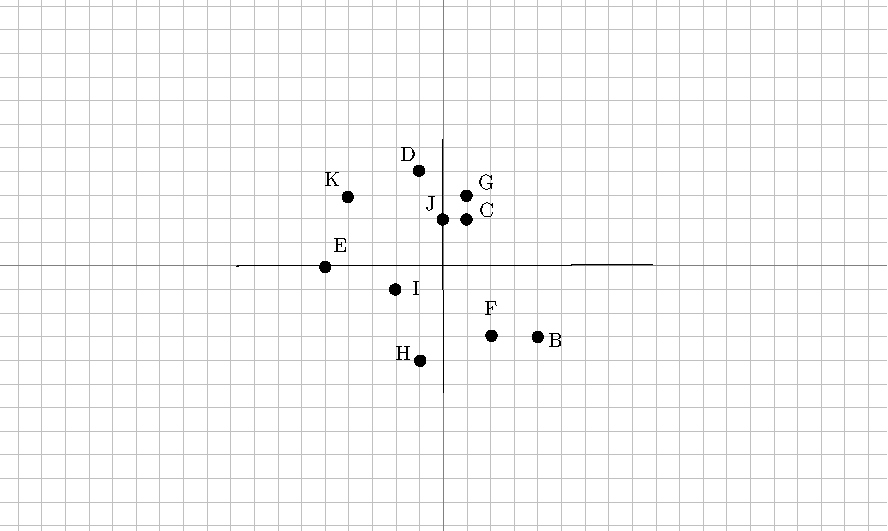
\includegraphics[scale=1,bb = 115 65 310 190, clip=true]{II_1_3bp-1.eps}
\end{multicols}

\

{\tmstrong{Plot each point.}}

2) L$(- 5, 5)$ \ \ \ \ \ \ K$(1, 0)$ \ \ \ \ \ \ \ \ J $(- 3, 4)$

\ \ \ \ I$(- 3, 0)$ \ \ \ \ \ \ \ H $(- 4, 2) \ \ \ \ $ G$(4, -2)$

\ \ \ \ F$(- 2, - 2)$ \ \ \ \ E $(3, - 2)$ \ \ \ \ D(0, 3)

\ \ \ \ C$(0, 4)$

\subsubsection{Graphing Lines from Points}\par

{\tmstrong{Sketch the graph of each line.}}

\begin{multicols}{2}
  1) $y = - \frac{1}{4} x - 3$
  
  3) $y = - \frac{5}{4} x - 4$
  
  5) $y = - 4 x + 2$
  
  7) $y = \frac{3}{2} x - 5$
  
  9) $y = - \frac{4}{5} x - 3$
  
  11) $x + 5 y = - 15$
  
  13) $4 x + y = 5$
  
  15) $2 x - y = 2$
  
  17) $x + y = - 1$
  
  19) $x - y = - 3$
  
  2) $y = x - 1$
  
  4) $y = - \frac{3}{5} x + 1$
  
  6) $y = \frac{5}{3} x + 4$
  
  8) $y = - x - 2$
  
  10) $y = \frac{1}{2} x$
  
  12) $8 x - y = 5$
  
  14) $3 x + 4 y = 16$
  
  16) $7 x + 3 y = - 12$
  
  18) $3 x + 4 y = 8$
  
  20) $9 x - y = - 4$
\end{multicols}

\pagebreak

\subsubsection{The Slope of a Line}\par

{\tmstrong{Find the slope of each line.}}
\label{lineargraphs1}
\begin{multicols}{2}
  1)\\
	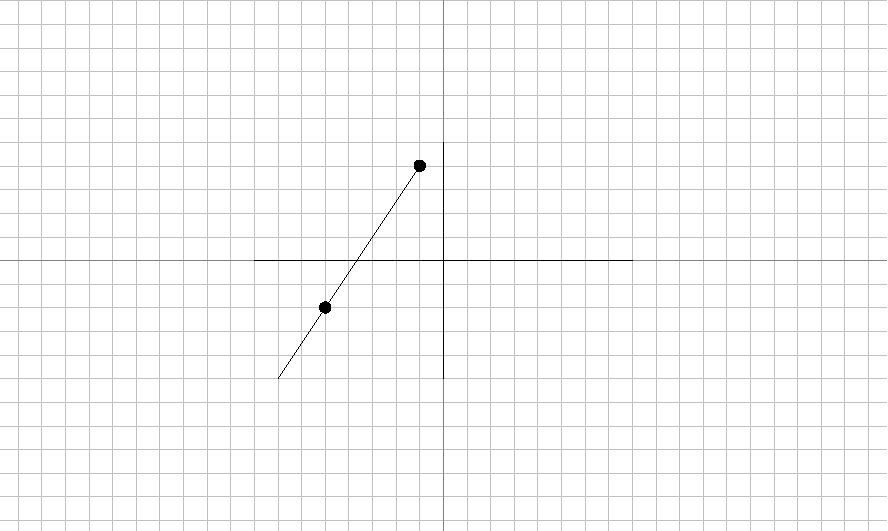
\includegraphics[scale=.8,bb = 115 65 310 190, clip=true]{II_1_3cp-1.eps}
  
  3)\\
	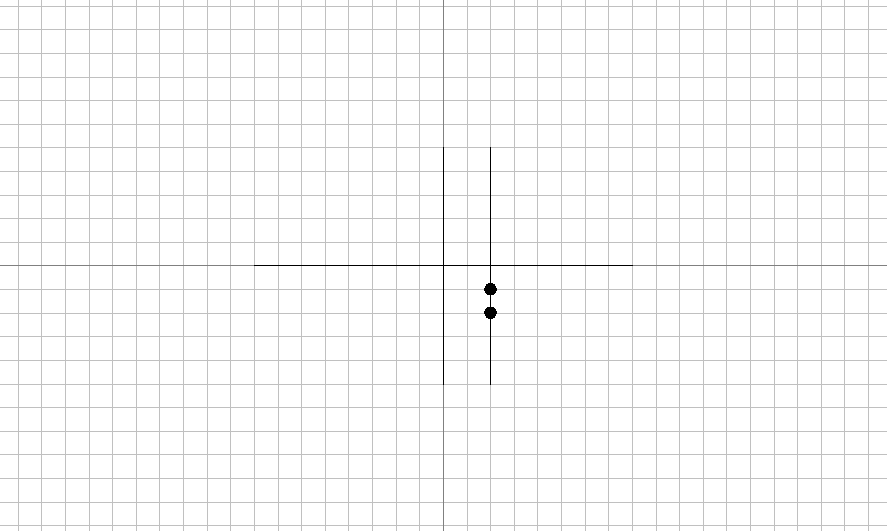
\includegraphics[scale=.8,bb = 115 65 310 190, clip=true]{II_1_3cp-2.eps}
  
  %5)\\
	%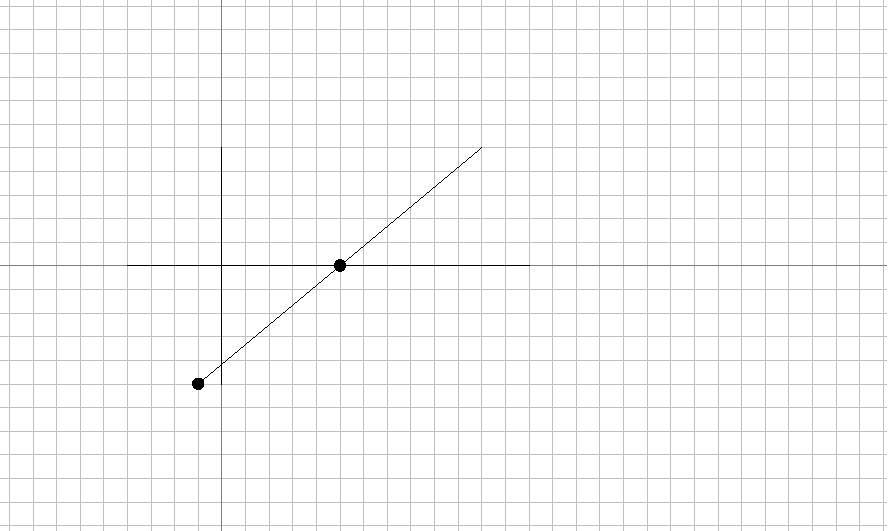
\includegraphics[scale=.8,bb = 115 65 310 190, clip=true]{II_1_3cp-3.eps}
  
%  7)\\
%	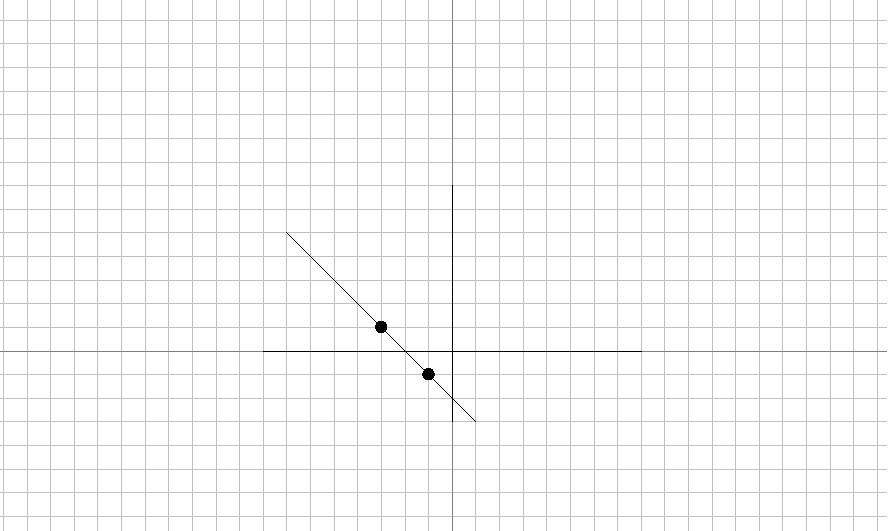
\includegraphics[scale=.8,bb = 115 65 310 190, clip=true]{II_1_3cp-4.eps}
  
%  \
  
  %2)\\
	%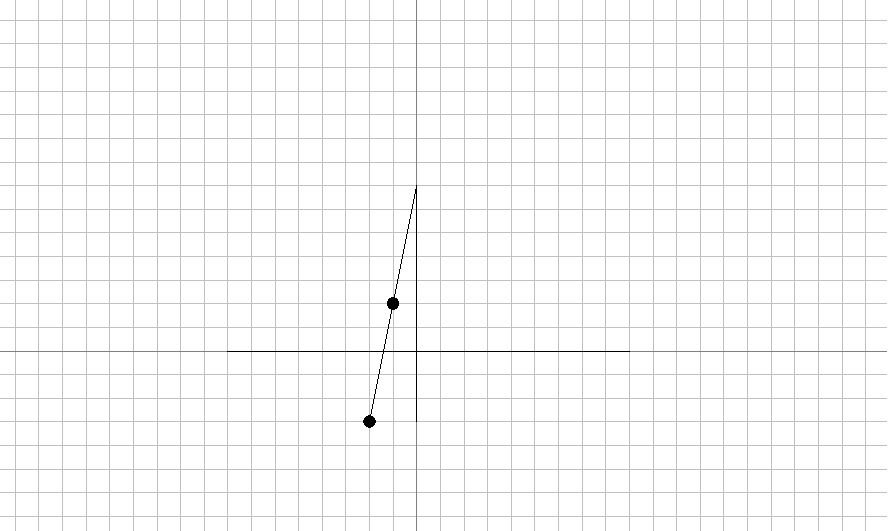
\includegraphics[scale=.8,bb = 115 65 310 190, clip=true]{II_1_3cp-5.eps}
  
  5)\\
	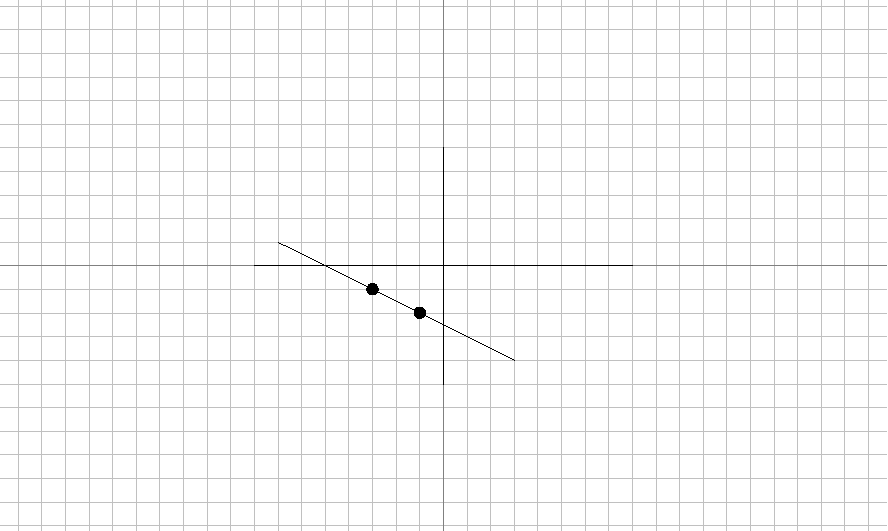
\includegraphics[scale=.8,bb = 115 65 310 190, clip=true]{II_1_3cp-6.eps}
  
  2)\\
	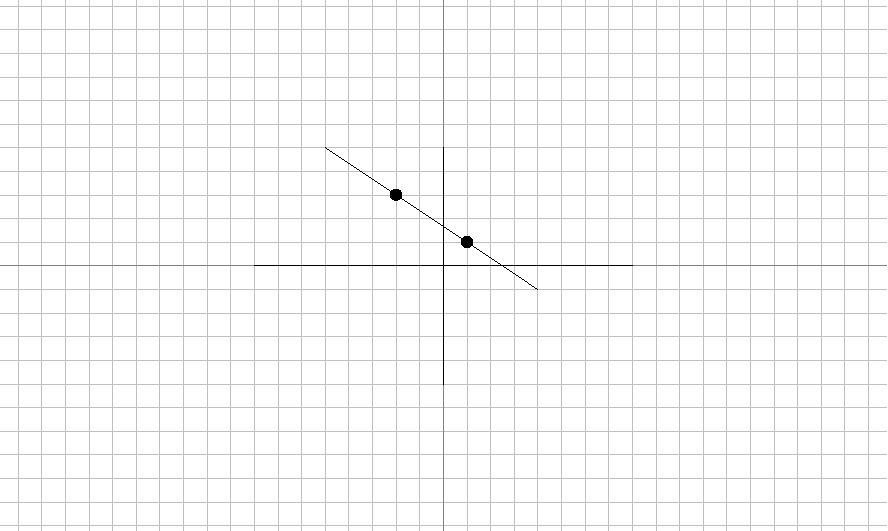
\includegraphics[scale=.8,bb = 115 65 310 190, clip=true]{II_1_3cp-7.eps}
  
%  8)\\
%	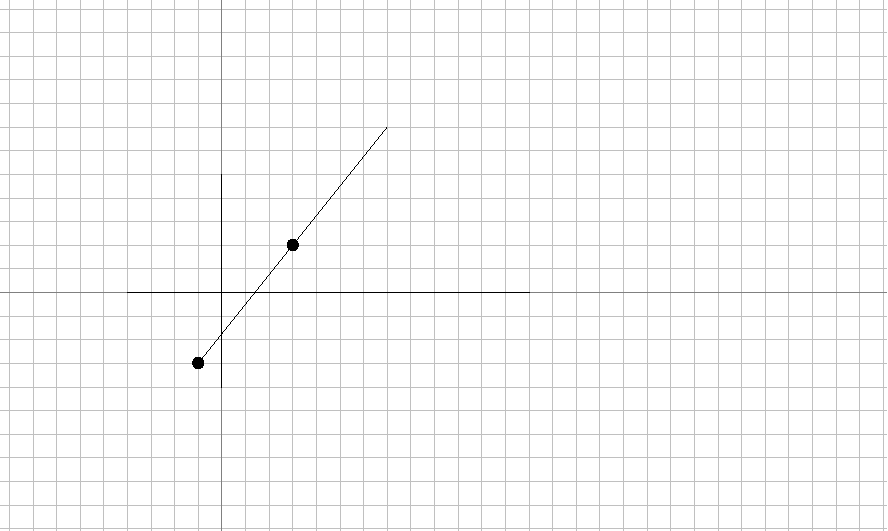
\includegraphics[scale=.8,bb = 115 65 310 190, clip=true]{II_1_3cp-8.eps}
  
  %{\pagebreak}
  
  4)\\
	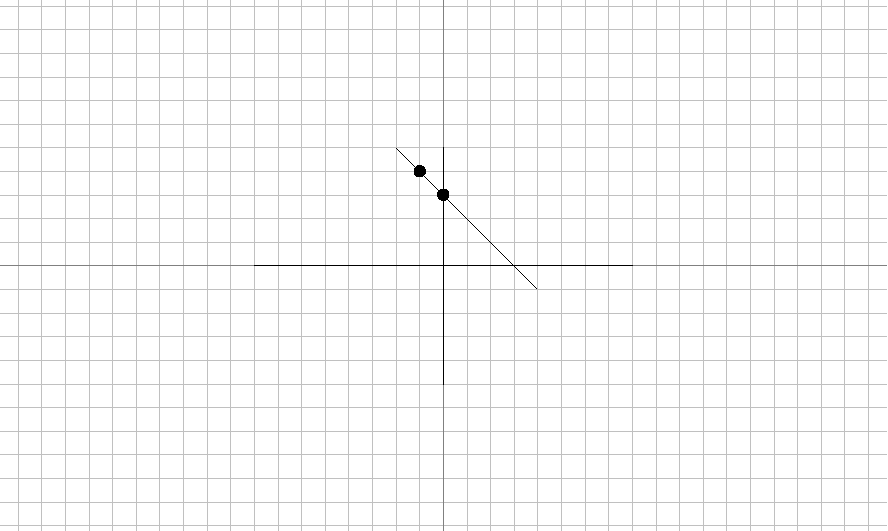
\includegraphics[scale=.8,bb = 115 65 310 190, clip=true]{II_1_3cp-9.eps}
  
  6)\\  
  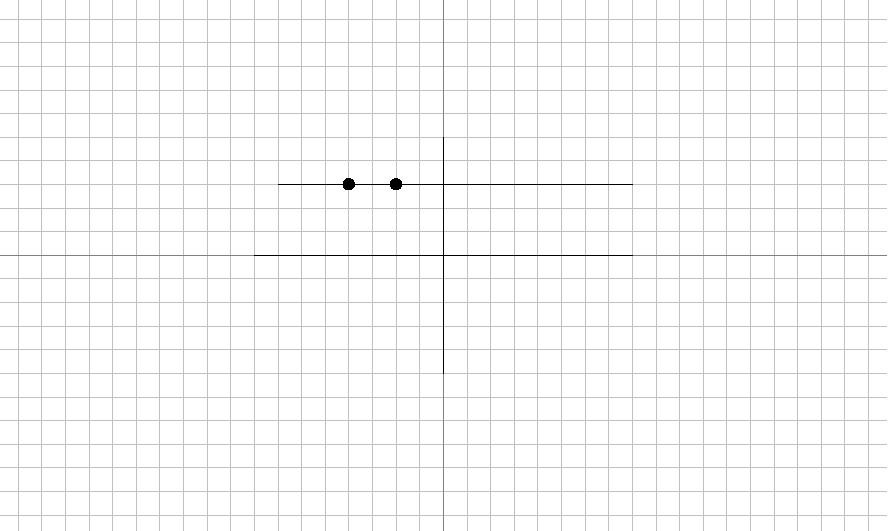
\includegraphics[scale=.8,bb = 115 65 310 190, clip=true]{II_1_3cp-10.eps}
\end{multicols}

\vspace{1in}
~

\pagebreak

{\tmstrong{Find the slope of the line through each pair of points.}}

\begin{multicols}{2}
  7) $(- 2, 10), (- 2, - 15)$
  
  9) $(- 15, 10), (16, - 7)$
  
  11) $(10, 18), (- 11, - 10)$
  
  13) $(- 16, - 14), (11, - 14)$
  
  15) $(- 4, 14), (- 16, 8)$
  
  17) $(12, - 19), (6, 14)$
  
  19) $(- 5, - 10), (- 5, 20)$
  
  21) $(- 17, 19), (10, - 7)$
  
  23) $(7, - 14), (- 8, - 9)$
  
  25) $(- 5, 7), (- 18, 14)$
  
  8) $(1, 2), (- 6, - 14)$
  
  10) $(13, - 2), (7, 7)$
  
  12) $(- 3, 6), (- 20, 13)$
  
  14) $(13, 15), (2, 10)$
  
  16) $(9, - 6), (- 7, - 7)$
  
  18) $(- 16, 2), (15, - 10)$
  
  20) $(8, 11), (- 3, - 13)$
  
  22) $(11, - 2), (1, 17)$
  
  24) $(- 18, - 5), (14, - 3)$
  
  26) $(19, 15), (5, 11)$
\end{multicols}

\

{\tmstrong{Find the value of x or y so that the line through the points has
the given slope.}}

\begin{multicols}{2}
  27) $(2, 6) \tmop{and} (x, 2) ; \tmop{slope} : \frac{4}{7}$
  
  29) $(- 3, - 2) \tmop{and} (x, 6) ; \tmop{slope} : - \frac{8}{5}$
  
  31) $(- 8, y) \tmop{and} (- 1, 1) ; \tmop{slope} : \frac{6}{7}$
  
  33) $(x, - 7) \tmop{and} (- 9, - 9) ; \tmop{slope} : \frac{2}{5}$
  
  35) $(x, 5) \tmop{and} (8, 0) ; \tmop{slope} : - \frac{5}{6}$
  
  28) $(8, y) \tmop{and} (- 2, 4) ; \tmop{slope} : - \frac{1}{5}$
  
  30) $(- 2, y) \tmop{and} (2, 4) ; \tmop{slope} : \frac{1}{4}$
  
  32) $(x, - 1) \tmop{and} (- 4, 6) ; \tmop{slope} : - \frac{7}{10}$
  
  34) $(2, - 5) \tmop{and} (3, y) ; \tmop{slope} : 6$
  
  36) $(6, 2) \tmop{and} (x, 6) ; \tmop{slope} : - \frac{4}{5}$
\end{multicols}

\vspace{2in}
~

\pagebreak

\subsection{The Two Forms of a Linear Equation}\par

	\subsubsection{Slope-Intercept Form}\par

{\tmstrong{Write the slope-intercept form of the equation of each line given
the slope and the y-intercept.}}

\begin{multicols}{2}
  1) Slope = 2, y-intercept = 5
  
  3) Slope = 1, y-intercept = $- 4$
  
  5) Slope = $- \frac{3}{4}$, y-intercept = $- 1$
  
  7) Slope = $\frac{1}{3}$, y-intercept = 1
  
  2) Slope = $- 6$, y-intercept = 4
  
  4) Slope = $- 1$, y-intercept = $- 2$
  
  6) Slope = $- \frac{1}{4}$, y-intercept = 3
  
  8) Slope = $\frac{2}{5}$, y-intercept = 5
\end{multicols}

{\tmstrong{Write the slope-intercept form of the equation of each line.}}

\begin{multicols}{2}
%  9)\\
%	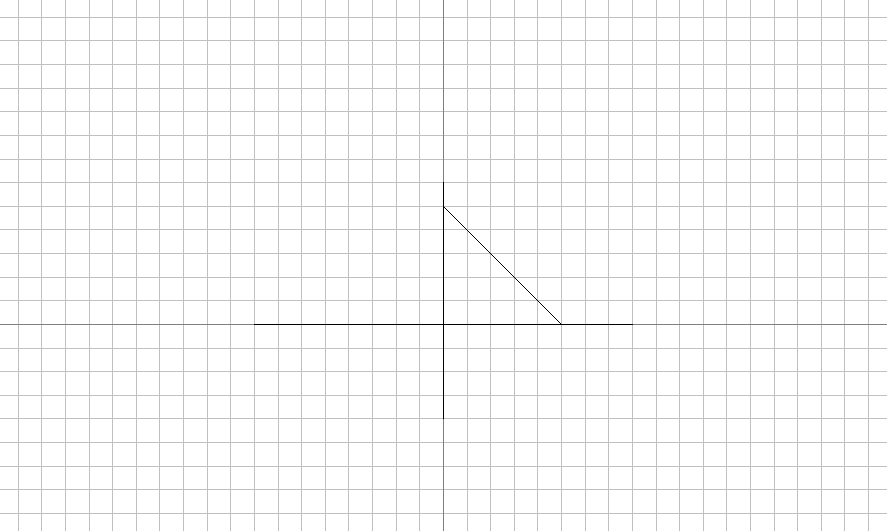
\includegraphics[scale=.7,bb = 115 65 310 190, clip=true]{II_1_4ap-1.eps}
  
  9)\\
	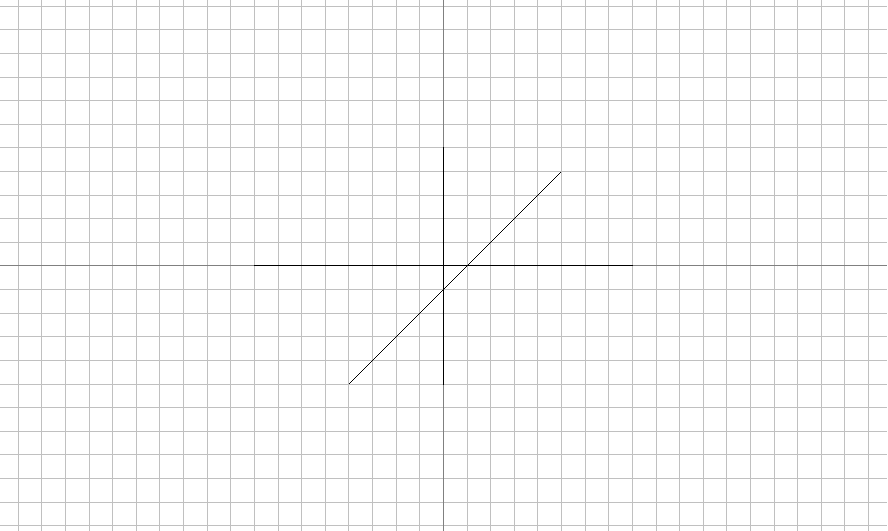
\includegraphics[scale=.7,bb = 115 65 310 190, clip=true]{II_1_4ap-2.eps}
  
  10)\\
	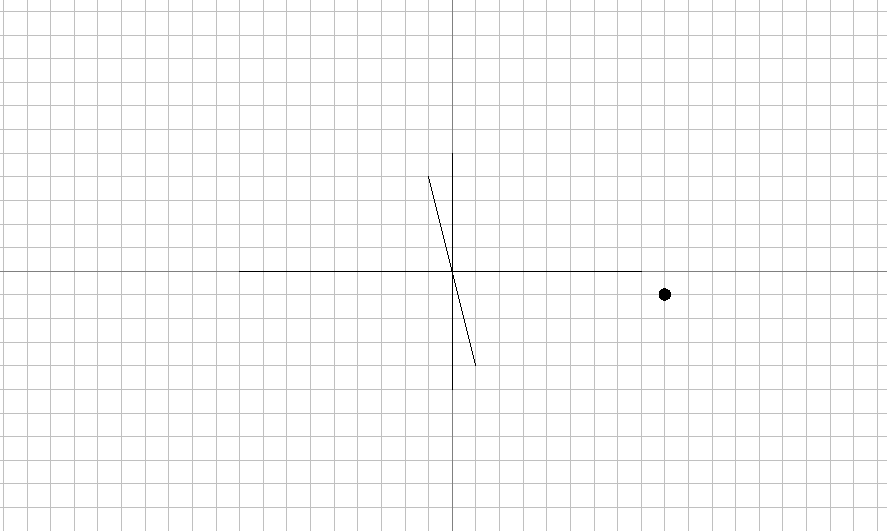
\includegraphics[scale=.7,bb = 115 65 310 190, clip=true]{II_1_4ap-3.eps}
  
 % 10)\\
%	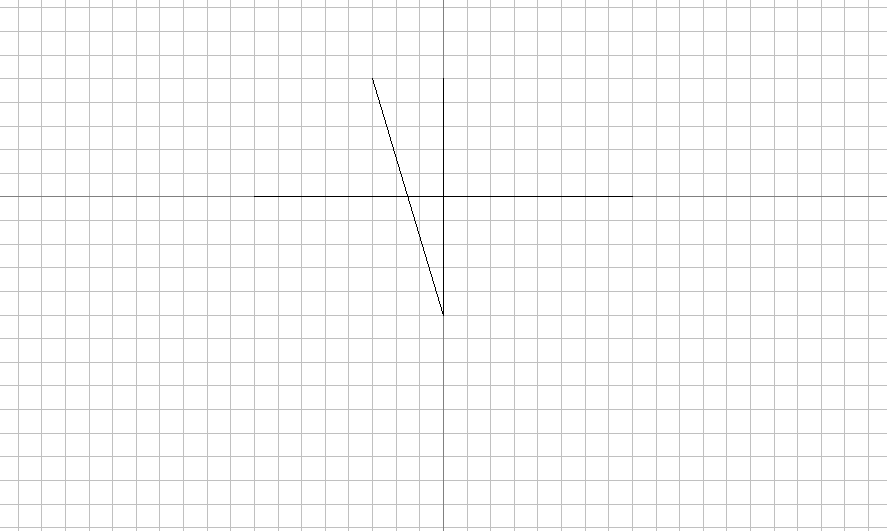
\includegraphics[scale=.7,bb = 115 65 310 190, clip=true]{II_1_4ap-4.eps}
  
 % 12)\\
%	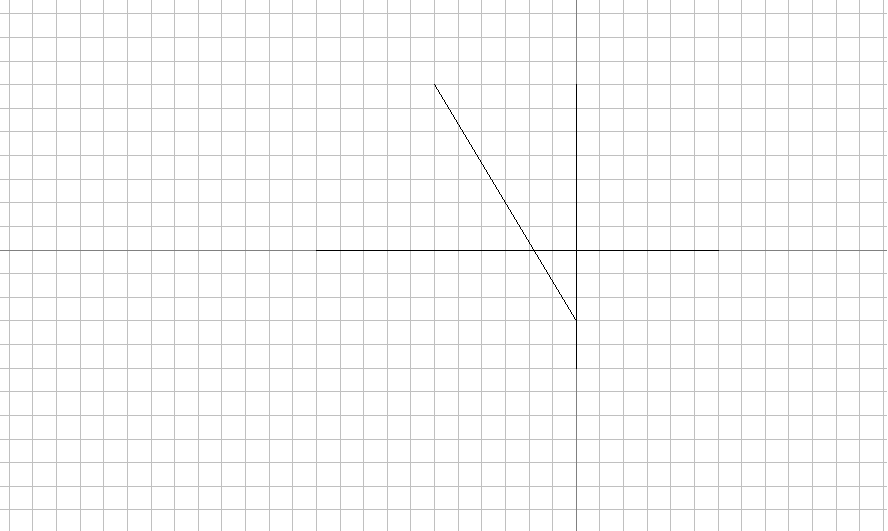
\includegraphics[scale=.7,bb = 115 65 310 190, clip=true]{II_1_4ap-5.eps}
  
 % 14)\\
%	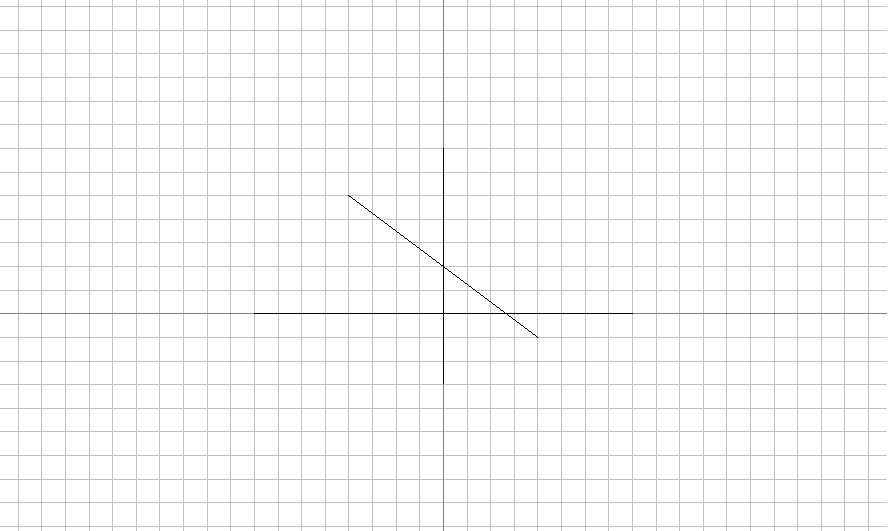
\includegraphics[scale=.7,bb = 115 65 310 190, clip=true]{II_1_4ap-6.eps}
\end{multicols}

%\pagebreak

{\tmstrong{Write each linear equation in slope-intercept form.}}

\begin{multicols}{2}
  11) $x + 10 y = - 37$
  
  13) $2 x + y = - 1$
  
  15) $7 x - 3 y = 24$
  
  17) $x = - 8$
  
  19) $y - 4 = - (x + 5)$
  
  21) $y - 4 = 4 (x - 1)$
  
  23) $y + 5 = - 4 (x - 2)$
  
  25) $y + 1 = - \frac{1}{2} (x - 4)$
  
  12) $x - 10 y = 3$
  
  14) $6 x - 11 y = - 70$
  
  16) $4 x + 7 y = 28$
  
  18) $x - 7 y = - 42$
  
  20) $y - 5 = \frac{5}{2} (x - 2)$
  
  22) $y - 3 = - \frac{2}{3} (x + 3)$
  
  24) $0 = x - 4$
  
  26) $y + 2 = \frac{6}{5} (x + 5)$
\end{multicols}

{\tmstrong{Sketch the graph of each line.}}
\label{lineargraphs2}
\begin{multicols}{2}
  27) $y = \frac{1}{3} x + 4$
  
  29) $y = \frac{6}{5} x - 5$
  
  31) $y = \frac{3}{2} x$
  
  33) $x - y + 3 = 0$
  
  35) $- y - 4 + 3 x = 0$
  
  37) $- 3 y = - 5 x + 9$
  
  28) $y = - \frac{1}{5} x - 4$
  
  30) $y = - \frac{3}{2} x - 1$
  
  32) $y = - \frac{3}{4} x + 1$
  
  34) $4 x + 5 = 5 y$
  
  36) $- 8 = 6 x - 2 y$
  
  38) $- 3 y = 3 - \frac{3}{2} x$
\end{multicols}

%\vspace{3in}
%~	

\pagebreak

	\subsubsection{Point-Slope Form}\par

{\tmstrong{Write the point-slope form of the equation of the line through the
given point with the given slope.}}

\begin{multicols}{2}
  1) $\tmop{through} (2, 3), \tmop{slope} = \tmop{undefined}$
  
  3) $\tmop{through} (2, 2), \tmop{slope} = \frac{1}{2}$
  
  5) $\tmop{through} (- 1, - 5), \tmop{slope} =$9
  
  7) $\tmop{through} (- 4, 1), \tmop{slope} = \frac{3}{4}$
  
  9) $\tmop{through} (0, - 2), \tmop{slope} = - 3$
  
  11) $\tmop{through} (0, - 5), \tmop{slope} = - \frac{1}{4}$
  
  13) $\tmop{through} (- 5, - 3), \tmop{slope} = \frac{1}{5}$
  
  15) $\tmop{through} (- 1, 4), \tmop{slope} = - \frac{5}{4}$
  
  2) $\tmop{through} (1, 2), \tmop{slope} =$undefined
  
  4) $\tmop{through} (2, 1), \tmop{slope} = - \frac{1}{2}$
  
  6) $\tmop{through} (2, - 2), \tmop{slope} = - 2$
  
  8) $\tmop{through} (4, - 3), \tmop{slope} = - 2$
  
  10) $\tmop{through} (- 1, 1), \tmop{slope} = 4$
  
  12) $\tmop{through} (0, 2), \tmop{slope} = - \frac{5}{4}$
  
  14) $\tmop{through} (- 1, - 4), \tmop{slope} = - \frac{2}{3}$
  
  16) $\tmop{through} (1, - 4), \tmop{slope} = - \frac{3}{2}$
\end{multicols}

\

{\tmstrong{Write the slope-intercept form of the equation of the line through
the given point with the given slope.}}

\begin{multicols}{2}
  17) through: $(- 1, - 5), \tmop{slope} = 2$
  
  19) through: $(5, - 1), \tmop{slope} = - \frac{3}{5}$
  
  21) through: $(- 4, 1), \tmop{slope} = \frac{1}{2}$
  
  23) through: $(4, - 2), \tmop{slope} = - \frac{3}{2}$
  
  25) through: $(- 5, - 3), \tmop{slope} = - \frac{2}{5}$
  
  27) through: $(2, - 2), \tmop{slope} = 1$
  
  29) through:$(- 3, 4)$, slope=undefined
  
  31) through: $(- 4, 2), \tmop{slope} = - \frac{1}{2}$
  
  18) through: $(2, - 2), \tmop{slope} = - 2$
  
  20) through: $(- 2, - 2), \tmop{slope} = - \frac{2}{3}$
  
  22) through: $(4, - 3), \tmop{slope} = - \frac{7}{4}$
  
  24) through: $(- 2, 0), \tmop{slope} = - \frac{5}{2}$
  
  26) through: $(3, 3), \tmop{slope} = \frac{7}{3}$
  
  28) through: $(- 4, - 3), \tmop{slope} =$0
  
  30) through: $(- 2, - 5), \tmop{slope} =$2
  
  32) through: $(5, 3), \tmop{slope} = \frac{6}{5}$
\end{multicols}

\

{\pagebreak}

{\tmstrong{Write the point-slope form of the equation of the line through the
given points.}}

\begin{multicols}{2}
  33) through: $(- 4, 3) \tmop{and} (- 3, 1)$
  
  35) through: $(5, 1) \tmop{and} (- 3, 0)$
  
  37) through: $(- 4, - 2) \tmop{and} (0, 4)$
  
  39) through: $(3, 5) \tmop{and} (- 5, 3)$
  
  41) through: $(3, - 3) \tmop{and} (- 4, 5)$
  
  34) through: $(1, 3) \tmop{and} (- 3, 3)$
  
  36) through: $(- 4, 5) \tmop{and} (4, 4)$
  
  38) through: $(- 4, 1) \tmop{and} (4, 4)$
  
  40) through: $(- 1, - 4) \tmop{and} (- 5, 0)$
  
  42) through: $(- 1, - 5) \tmop{and} (- 5, - 4)$
\end{multicols}

\

{\tmstrong{Write the slope-intercept form of the equation of the line through
the given points.}}

\begin{multicols}{2}
  43) through: $(- 5, 1) \tmop{and} (- 1, - 2)$
  
  45) through: $(- 5, 5) \tmop{and} (2, - 3)$
  
  47) through: $(4, 1) \tmop{and} (1, 4)$
  
  49) through: $(0, 2) \tmop{and} (5, - 3)$
  
  51) through: $(0, 3) \tmop{and} (- 1, - 1)$
  
  44) through: $(- 5, - 1) \tmop{and} (5, - 2)$
  
  46) through: $(1, - 1) \tmop{and} (- 5, - 4)$
  
  48) through: $(0, 1) \tmop{and} (- 3, 0)$
  
  50) through: $(0, 2) \tmop{and} (2, 4)$
  
  52) through: $(- 2, 0) \tmop{and} (5, 3)$
\end{multicols}

\vspace{2in}
~

\pagebreak

\subsection{Parallel and Perpendicular Lines}\par

{\tmstrong{Find the slope of a line parallel to each given line.}}

\begin{multicols}{2}
  1) $y = 2 x + 4$
  
  3) $y = 4 x - 5$
  
  5) $x - y = 4$
  
  7) $7 x + y = - 2$
  
  2) $y = - \frac{2}{3} x + 5$
  
  4) $y = - \frac{10}{3} x - 5$
  
  6) $6 x - 5 y = 20$
  
  8) $3 x + 4 y = - 8$
\end{multicols}

\

{\tmstrong{Find the slope of a line perpendicular to each given line.}}

\begin{multicols}{2}
  9) $x = 3$
  
  11) $y = - \frac{1}{3} x$
  
  13) $x - 3 y = - 6$
  
  15) $x + 2 y = 8$
  
  10) $y = - \frac{1}{2} x - 1$
  
  12) $y = \frac{4}{5} x$
  
  14) $3 x - y = - 3$
  
  16) $8 x - 3 y = - 9$
\end{multicols}

\

{\tmstrong{Write the point-slope form of the equation of the line
described.}}

17) $\tmop{through} : (2, 5), \tmop{parallel} \tmop{to} x = 0$

18) through: (5, 2), parallel to $y = \frac{7}{5} x + 4$

19) $\tmop{through} : (3, 4), \tmop{parallel} \tmop{to} y = \frac{9}{2} x - 5$

20) through: $(1, - 1), \tmop{parallel} \tmop{to} y = - \frac{3}{4} x + 3$

21) $\tmop{through} : (2, 3), \tmop{parallel} \tmop{to} y = \frac{7}{5} x + 4$

22) $\tmop{through} : (- 1, 3), \tmop{parallel} \tmop{to} y = - 3 x - 1$

23) $\tmop{through} : (4, 2), \tmop{parallel} \tmop{to} x = 0$

24) $\tmop{through} : (1, 4), \tmop{parallel} \tmop{to} y = \frac{7}{5} x + 2$

25) through: (1, $- 5), \tmop{perpendicular} \tmop{to} - x + y = 1$

26) $\tmop{through} : (1, - 2), \tmop{perpendicular} \tmop{to} - x + 2 y = 2$

27) $\tmop{through} : (5, 2), \tmop{perpendicular} \tmop{to} 5 x + y = - 3$

28) through: (1, 3), $\tmop{perpendicular} \tmop{to} - x + y = 1$

29) $\tmop{through} : (4, 2), \tmop{perpendicular} \tmop{to} - 4 x + y = 0$

30) through: $(- 3, - 5), \tmop{perpendicular} \tmop{to} 3 x + 7 y = 0$

31) $\tmop{through} : (2, - 2) \tmop{perpendicular} \tmop{to} 3 y - x = 0$

32) through: $(- 2, 5) . \tmop{perpendicular} \tmop{to} y - 2 x = 0$

\pagebreak

{\tmstrong{Write the slope-intercept form of the equation of the line
described.}}

33) $\tmop{through} : (4, - 3), \tmop{parallel} \tmop{to} y = - 2 x$

34) $\tmop{through} : (- 5, 2), \tmop{parallel} \tmop{to} y = \frac{3}{5} x$

35) $\tmop{through} : (- 3, 1), \tmop{parallel} \tmop{to} y = - \frac{4}{3} x
- 1$

36) $\tmop{through} : (- 4, 0), \tmop{parallel} \tmop{to} y = - \frac{5}{4} x
+ 4$

37) $\tmop{through} : (- 4, - 1), \tmop{parallel} \tmop{to} y = - \frac{1}{2}
x + 1$

38) $\tmop{through} : (2, 3), \tmop{parallel} \tmop{to} y = \frac{5}{2} x - 1$

39) $\tmop{through} : (- 2, - 1), \tmop{parallel} \tmop{to} y = - \frac{1}{2}
x - 2$

40) $\tmop{through} : (- 5, - 4), \tmop{parallel} \tmop{to} y = \frac{3}{5} x
- 2$

41) $\tmop{through} : (4, 3), \tmop{perpendicular} \tmop{to} x + y = - 1$

42) $\tmop{through} : (- 3, - 5), \tmop{perpendicular} \tmop{to} x + 2 y = -
4$

43) $\tmop{through} : (5, 2), \tmop{perpendicular} \tmop{to} x = 0$

44) $\tmop{through} : (5, - 1), \tmop{perpendicular} \tmop{to} - 5 x + 2 y =
10$

45) $\tmop{through} : (- 2, 5), \tmop{perpendicular} \tmop{to} - x + y = - 2$

46) $\tmop{through} : (2, - 3), \tmop{perpendicular} \tmop{to} - 2 x + 5 y = -
10$

47) $\tmop{through} : (4, - 3), \tmop{perpendicular} \tmop{to} - x + 2 y = -
6$

48) $\tmop{through} : (- 4, 1), \tmop{perpendicular} \tmop{to} 4 x + 3 y = -
9$

\vspace{3in}
~

\pagebreak

\subsection{Applications}\par

	\subsubsection{Numbers and Geometry}\par

{\tmstrong{Solve.}}

1. When five is added to three more than a certain number, the result is 19.  What is the number?

2. If five is subtracted from three times a certain number, the result is
$10$. What is the number?

3. When 18 is subtracted from six times a certain number, the result is $-
42$. What is the number?

4. A certain number added twice to itself equals 96. What is the number?

5. A number plus itself, plus twice itself, plus 4 times itself, is equal to
$- 104$. What is the number?

6. Sixty more than nine times a number is the same as two less than ten times
the number. What is the number?

7. Eleven less than seven times a number is five more than six times the
number. Find the number.

8. Fourteen less than eight times a number is three more than four times the number. What is the number?

9. The sum of three consecutive integers is 108. What are the integers?

10. The sum of three consecutive integers is $- 126$. What are the integers?

11. Find three consecutive integers such that the sum of the first, twice the
second, and three times the third is $- 76$.

12. The sum of two consecutive even integers is 106. What are the integers?

13. The sum of three consecutive odd integers is 189. What are the integers?

14. The sum of three consecutive odd integers is 255. What are the integers?

15. Find three consecutive odd integers such that the sum of the first, two
times the second, and three times the third is 70.

16. The second angle of a triangle is the same size as the first angle. The
third angle is 12 degrees larger than the first angle. How
large are the angles?

17. Two angles of a triangle are the same size. The third angle is 12 degrees
smaller than the first angle. Find the measure of the
angles.

18. Two angles of a triangle are the same size. The third angle is 3 times as
large as the first. How large are the angles?

19. The third angle of a triangle is the same size as the first. The second
angle is 4 times the third. Find the measure of the angles.

\pagebreak

20. The second angle of a triangle is 3 times as large as the first angle. The
third angle is 30 degrees more than the first angle. Find the
measure of the angles.

21. The second angle of a triangle is twice as large as the first. The measure
of the third angle is 20 degrees greater than the first. How
large are the angles?

22. The second angle of a triangle is three times as large as the first. The
measure of the third angle is 40 degrees greater than that of the
first angle. How large are the three angles?

23. The second angle of a triangle is five times as large as the first. The
measure of the third angle is 12 degrees greater than that of
the first angle. How large are the angles?

24. The second angle of a triangle is three times the first, and the third is
12 degrees less than twice the first. Find the
measures of the angles.

25. The second angle of a triangle is four times the first and the third is 5
degrees more than twice the first. Find the measures of the angles.

26. The perimeter of a rectangle is 150 cm. The length is 15 cm greater than
the width. Find the dimensions.

27. The perimeter of a rectangle is 304 cm. The length is 40 cm longer than
the width. Find the length and width.

28. The perimeter of a rectangle is 152 meters. The width is 22 meters less
than the length. Find the length and width.

29. The perimeter of a rectangle is 280 meters. The width is 26 meters less
than the length. Find the length and width.

30. The perimeter of a college basketball court is 96 meters and the length is
14 meters more than the width. What are the dimensions?

31. A mountain cabin on 1 acre of land costs $\$30,000$. If the land
cost 4 times as much as the cabin, what was the cost of each?

32. A horse and a saddle cost $\$5000$. If the horse cost 4 times as
much as the saddle, what was the cost of each?

33. A bicycle and a bicycle helmet cost $\$240$. How much did each
cost, if the bicycle cost 5 times as much as the helmet?

34. Of 240 stamps that Harry and his sister collected, Harry collected 3 times
as many as his sisters. How many did each collect?

35. If Mr. Brown and his son together had $\$220$, and Mr. Brown had
10 times as much as his son, how much money had each?

36. In a room containing 45 students there were twice as many girls as boys.
How many of each were there?

37. Aaron had 7 times as many sheep as Beth, and both together had 608. How many sheep had each?

\pagebreak

38. A man bought a cow and a calf for $\$990$, paying 8 times as much
for the cow as for the calf. What was the cost of each?

39. Jamal and Moshe began a business with a capital of $\$7500$. If
Jamal furnished half as much capital as
Moshe, how much did each furnish?

40. A lab technician cuts a 12 inch piece of tubing into two pieces in such a
way that one piece is 2 times longer than the other.

41. A 6 ft board is cut into two pieces, one twice as long as the other. How
long are the pieces?

42. An eight ft board is cut into two pieces. One piece is 2 ft longer than
the other. How long are the pieces?

43. An electrician cuts a 30 ft piece of wire into two pieces. One piece is 2
ft longer than the other. How long are the pieces?

44. The total cost for tuition plus room and board at State University is
$\$2,584$. Tuition costs $\$704$ more than
room and board. What is the tuition fee?

45. The cost of a private pilot course is $\$1,275$. The flight
portion costs $\$625$ more than the groung
school portion. What is the cost of each?

\vspace{4in}
~

\pagebreak

	\subsubsection{Age Problems}\par

1. A boy is 10 years older than his brother. In 4 years he will be twice as
old as his brother. Find the present age of each.

2. A father is 4 times as old as his son. In 20 years the father will be
twice as old as his son. Find the present age of each.

3. Pat is 20 years older than his son James. In two years Pat will be twice as
old as James. How old are they now?

4. Diane is 23 years older than her daughter Amy. In 6 years Diane will be
twice as old as Amy. How old are they now?

5. Fred is 4 years older than Barney. Five years ago the sum of their ages was
48. How old are they now?

6. John is four times as old as Martha. Five years ago the sum of their ages
was 50. How old are they now?

7. Tim is 5 years older than JoAnn. Six years from now the sum of their ages
will be 79. How old are they now?

8. Jack is twice as old as Lacy. In three years the sum of their ages will be
54. How old are they now?

9. The sum of the ages of John and Mary is 32. Four years ago, John was twice
as old as Mary. Find the present age of each.

10. The sum of the ages of a father and son is 56. Four years ago the father
was 3 times as old as the son. Find the present age of each.

11. The sum of the ages of a china plate and a glass plate is 16 years. Four
years ago the china plate was three times the age of the glass
plate. Find the present age of each plate.

12. The sum of the ages of a wood plaque and a bronze plaque is 20 years. Four
years ago, the bronze plaque was one-half the age of the wood
plaque. Find the present age of each plaque.

13. Adam is now 34 years old, and Bryce is 4 years old. In how many years will Adam be twice as old as Bryce?

14. A man's age is 36 and that of his daughter is 3 years. In how many years
will the man be 4 times as old as his daughter?

15. An Oriental rug is 52 years old and a Persian rug is 16 years old. How
many years ago was the Oriental rug four times as old as the
Persian Rug?

16. A log cabin quilt is 24 years old and a friendship quilt is 6 years old.
In how may years will the log cabin quilt be three times as old
as the friendship quilt?

17. The age of the older of two boys is twice that of the younger; 5 years ago
it was three times that of the younger. Find the age of
each.

18. A pitcher is 30 years old, and a vase is 22 years old. How many years ago
was the pitcher twice as old as the vase?

19. Marge is twice as old as Consuelo. The sum of their ages seven years ago
was 13. How old are they now?

20. The sum of Jason and Mandy's age is 35. Ten years ago Jason was double Mandy's age. How old are they now?

21. A silver coin is 28 years older than a bronze coin. In 6 years, the silver
coin will be twice as old as the bronze coin. Find the
present age of each coin.

22. A sofa is 12 years old and a table is 36 years old. In how many years will
the table be twice as old as the sofa?

23. A limestone statue is 56 years older than a marble statue. In 12 years,
the limestone will be three times as old as the marble
statue. Find the present age of the statues.

24. A pewter bowl is 8 years old, and a silver bowl is 22 years old. In how
many years will the silver bowl be twice the age of the pewter
bowl?

25. Brandon is 9 years older than Ronda. In four years the sum of their ages
will be 91. How old are they now?

26. A kerosene lamp is 95 years old, and an electric lamp is 55 years old. How
many years ago was the kerosene lamp twice the age of the
electric lamp?

27. A father is three times as old as his son, and his daughter is 3 years
younger than the son. If the sum of their ages 3 years ago
was 63 years, find the present age of the father.

28. The sum of Clyde and Wendy's age is 64. In four years, Wendy will be three
times as old as Clyde. How old are they now?

29. The sum of the ages of two ships is 12 years. Two years ago, the age of
the older ship was three times the age of the newer ship.
Find the present age of each ship.

30. Chelsea's age is double Daniel's age. Eight years ago the sum of their
ages was 32. How old are they now?

31. Ann is eighteen years older than her son. One year ago, she was three
times as old as her son. How old are they now?

32. The sum of the ages of Kristen and Ben is 32. Four years ago Kristen was twice as old as Ben. How old are they both now?

33. A mosaic is 74 years older than the engraving. Thirty years ago, the
mosaic was three times as old as the engraving. Find the
present age of each.

34. The sum of the ages of Elli and Dan is 56. Four years ago Elli was 3 times
as old as Dan. How old are they now?

35. A wool tapestry is 32 years older than a linen tapestry. Twenty years ago,
the wool tapestry was twice as old as the linen tapestry. Find the
present age of each.

36. Carolyn's age is triple her daughter's age. In eight years the sum of
their ages will be 72. How old are they now?

37. Nicole is 26 years old. Emma is 2 years old. In how many years will Nicole
be triple Emma's age?

38. The sum of the ages of two children is 16 years. Four years ago, the age
of the older child was three times the age of the younger child.
Find the present age of each child.

39. Mike is 4 years older than Ron. In two years, the sum of their ages will
be 84. How old are they now?

40. A marble bust is 25 years old, and a terra-cotta bust is 85 years old. In
how many years will the terra-cotta bust be three times as old
as the marble bust?

\vspace{4in}
~


\pagebreak

	\subsubsection{Distance, Rate and Time}\par

1. A is 60 miles from B. An automobile at A starts for B at the rate of 20
miles an hour at the same time that an automobile at B starts
for A at the rate of 25 miles an hour. How long will it be
before the automobiles meet?

2. Two automobiles are 276 miles apart and start at the same time to travel toward each other. They travel at rates differing by 5
miles per hour. If they meet after 6 hours, find the rate of
each.

3. Two trains travel toward each other from points which are 195 miles apart.
They travel at rate of 25 and 40 miles an hour respectively.
If they start at the same time, how soon will they meet?

4. A and B start toward each other at the same time from points 150 miles
apart. If A went at the rate of 20 miles an hour, at what rate must B
travel if they meet in 5 hours?

5. A passenger and a freight train start toward each other at the same time
from two points 300 miles apart. If the rate of the passenger train
exceeds the rate of the freight train by 15 miles per hour, and
they meet after 4 hours, what must the rate of each be?

6. Two automobiles started at the same time from a point, but traveled in opposite directions. Their rates were 25 and 35 miles
per hour respectively. After how many hours were they 180
miles apart?

7. A man having ten hours at his disposal made an excursion, riding out at the
rate of 10 miles an hour and returning on foot, at the rate of
3 miles an hour. Find the distance he rode.

8. A man walks at the rate of 4 miles per hour. How far can he walk into the country and ride back on a trolley that travels at the rate
of 20 miles per hour, if he must be back home 3 hours from the time he
started?

9. A boy rides away from home in an automobile at the rate of 28 miles an hour
and walks back at the rate of 4 miles an hour. The round trip
requires 2 hours. How far does he ride?

10. A motorboat leaves a harbor and travels at an average speed of 15 mph toward an island. The average speed on the return trip
was 10 mph. How far was the island from the harbor if the total
trip took 5 hours?

11. A family drove to a resort at an average speed of 30 mph and later
returned over the same road at an average speed of 50 mph.
Find the distance to the resort if the total driving time was
8 hours.

12. As part of his flight training, a student pilot was required to fly to an
airport and then return. The average speed to the airport was 90
mph, and the average speed returning was 120 mph.
Find the distance between the two airports if the total
flying time was 7 hours.

13. A, who travels 4 miles an hour starts from a certain place 2 hours in
advance of B, who travels 5 miles an hour in the same direction.
How many hours must B travel to overtake A?

14. A man travels 5 miles an hour. After traveling for 6 hours another man
starts at the same place, following at the rate of 8 miles an hour.
When will the second man overtake the first?

15. A motorboat leaves a harbor and travels at an average speed of 8 mph
toward a small island. Two hours later a cabin cruiser leaves the
same harbor and travels at an average speed of 16 mph
toward the same island. In how many hours after the cabin
cruiser leaves will the cabin cruiser be alongside the motorboat?

16. A long distance runner started on a course running at an average speed of
6 mph. One hour later, a second runner began the same course
at an average speed of 8 mph. How long after the second
runner started will the second runner overtake the first
runner?

17. A car traveling at 48 mph overtakes a cyclist who, riding at 12 mph, has
had a 3 hour head start. How far from the starting point does
the car overtake the cyclist?

18. A jet plane traveling at 600 mph overtakes a propeller-driven plane which
has had a 2 hour head start. The propeller-driven plane is
traveling at 200 mph. How far from the starting point does the
jet overtake the propeller-driven plane?

19. Two men are traveling in opposite directions at the rate of 20 and 30
miles an hour at the same time and from the same place. In how
many hours will they be 300 miles apart?

20. Running at an average rate of 8 m/s, a sprinter ran to the end of a track
and then jogged back to the starting point at an average rate of
3 m/s. The sprinter took 55 s to run to the end of
the track and jog back. Find the length of the
track.

21. A motorboat leaves a harbor and travels at an average speed of 18 mph to
an island. The average speed on the return trip was 12 mph. How
far was the island from the harbor if the total trip took
5 h?

22. A motorboat leaves a harbor and travels at an average speed of 9 mph
toward a small island. Two hours later a cabin cruiser leaves the
same harbor and travels at an average speed of 18 mph
toward the same island. In how many hours after the cabin
cruiser leaves will the cabin cruiser be alongside the motorboat?

\pagebreak

23. A jet plane traveling at 570 mph overtakes a propeller-driven plane that
has had a 2 h head start. The propeller-driven plane is
traveling at 190 mph. How far from the starting point
does the jet overtake the propeller-driven plane?

24. Two trains start at the same time from the same place and travel in
opposite directions. If the rate of one is 6 miles per hour more
than the rate of the other and they are 168 miles apart
at the end of 4 hours, what is the rate of each?

25. As part of flight training, a student pilot was required to fly to an
airport and then return. The average speed on the way to the
airport was 100 mph, and the average speed returning was 150
mph. Find the distance between the two airports if the total
flight time was 5 h.

26. Two cyclists start from the same point and ride in opposite directions.
One cyclist rides twice as fast as the other. In three
hours they are 72 miles apart. Find the rate of each cyclist.

27. A car traveling at 56 mph overtakes a cyclist who, riding at 14 mph, has
had a 3 h head start. How far from the starting point does the
car overtake the cyclist?

28. Two small planes start from the same point and fly in opposite directions.
The first plan is flying 25 mph slower than the second
plane. In two hours the planes are 430 miles apart. Find
the rate of each plane.

29. A bus traveling at a rate of 60 mph overtakes a car traveling at a rate of
45 mph. If the car had a 1 h head start, how far from the
starting point does the bus overtake the car?

30. Two small planes start from the same point and fly in opposite directions.
The first plane is flying 25 mph slower than the second
plane. In 2 h, the planes are 470 mi apart. Find the
rate of each plane.

31. A truck leaves a depot at 11 A.M. and travels at a speed of 45 mph. At
noon, a van leaves the same place and travels the same route at a
speed of 65 mph. At what time does the van overtake the truck?

32. A family drove to a resort at an average speed of 25 mph and later
returned over the same road at an average speed of 40 mph.
Find the distance to the resort if the total driving time was
13 h.

33. Three campers left their campsite by canoe and paddled downstream at an average rate of 10 mph. They then turned around and paddled
back upstream at an average rate of 5 mph
to return to their campsite. How long did it take the campers
to canoe downstream if the total trip took 1 hr?

\pagebreak

34. A motorcycle breaks down and the rider has to walk the rest of the way to
work. The motorcycle was being driven at 45 mph, and the
rider walks at a speed of 6 mph. The distance from home to
work is 25 miles, and the total time for the trip was 2
hours. How far did the motorcycle go before if broke down?

35. A student walks and jogs to college each day. The student averages 5 km/hr
walking and 9 km/hr jogging. The distance from home to college
is 8 km, and the student makes the trip in one hour. How
far does the student jog?

36. On a 130 mi trip, a car traveled at an average speed of 55 mph and then reduced its speed to 40 mph for the remainder of the
trip. The trip took a total of 2.5 h. For how long did the
car travel at 40 mph?

37. On a 220 mi trip, a car traveled at an average speed of 50 mph and then reduced its average speed to 35 mph for the remainder
of the trip. The trip took a total of 5 h. How long did the
car travel at each speed?

38. An executive drove from home at an average speed of 40 mph to an airport where a helicopter was waiting. The executive boarded the
helicopter and flew to the corporate offices at and
average speed of 60 mph. The entire distance was 150
mi. The entire trip took 3 h. Find the distance from the airport to the corporate offices.

\vspace{3in}
~

\pagebreak

\subsection{Linear Inequalities and Sign Diagrams}\par

{\tmstrong{Draw a graph for each inequality and provide interval notation.}}

\begin{multicols}{2}
  1) $n > - 5$
  
  3) $- 2 \geq k$
  
  5) $5 \geq x$
  
  2) $n > 4$
  
  4) $1 \geq k$
  
  6) $- 5 < x$
\end{multicols}

\

%{\tmstrong{Write an inequality for each graph.}}

%\begin{multicols}{2}
%  7)
  
%  \resizebox{391px}{55px}{\includegraphics{Inequalities - graph and solve -
%  problem set-1.eps}}
  
%  8)
  
%  \resizebox{391px}{55px}{\includegraphics{Inequalities - graph and solve -
%  problem set-2.eps}}
  
%  9)
  
%  \resizebox{391px}{55px}{\includegraphics{Inequalities - graph and solve -
%  problem set-3.eps}}
  
%  10)
  
%  \resizebox{391px}{55px}{\includegraphics{Inequalities - graph and solve -
%  problem set-4.eps}}
  
%  11)
  
%  \resizebox{391px}{55px}{\includegraphics{Inequalities - graph and solve -
%  problem set-5.eps}}
  
%  12)
  
%  \resizebox{391px}{55px}{\includegraphics{Inequalities - graph and solve -
%  problem set-6.eps}}
%\end{multicols}

{\tmstrong{Solve each inequality, graph each solution, and provide interval
notation.}}

\begin{multicols}{2}
  7) $\frac{x}{11} \geq 10$
  
  9) $2 + r < 3$
  
  11) $8 + \frac{n}{3} \geq 6$
  
  13) $2 > \frac{a - 2}{5}$
  
  15) $- 47 \geq 8 - 5 x$
  
  17) $- 2 (3 + k) < - 44$
  
  19) $18 < - 2 (- 8 + p)$
  
  21) $24 \geq - 6 (m - 6)$
  
  23) $- r - 5 (r - 6) < - 18$
  
  25) $24 + 4 b < 4 (1 + 6 b)$
  
  27) $- 5 v - 5 < - 5 (4 v + 1)$
  
  29) $4 + 2 (a + 5) < - 2 (- a - 4)$
  
  31) $- (k - 2) > - k - 20$
  
  8) $- 2 \leq \frac{n}{13}$
  
  10) $\frac{m}{5} \leq - \frac{6}{5}$
  
  12) $11 > 8 + \frac{x}{2}$
  
  14) $\frac{v - 9}{- 4} \leq 2$
  
  16) $\frac{6 + x}{12} \leq - 1$
  
  18) $- 7 n - 10 \geq 60$
  
  20) $5 \geq \frac{x}{5} + 1$
  
  22) $- 8 (n - 5) \geq 0$
  
  24) $- 60 \geq - 4 (- 6 x - 3)$
  
  26) $- 8 (2 - 2 n) \geq - 16 + n$
  
  28) $- 36 + 6 x > - 8 (x + 2) + 4 x$
  
  30) $3 (n + 3) + 7 (8 - 8 n) < 5 n + 5 + 2$
  
  32) $- (4 - 5 p) + 3 \geq - 2 (8 - 5 p)$ 
\end{multicols}

{\tmstrong{Construct a sign diagram for each of following graphs/linear equations referenced below.}}\pp

33)-38): Graphs (1) through (6) on page \pageref{lineargraphs1}.\pp

39)-50): Linear equations (27) through (38) on page \pageref{lineargraphs2}.\pp

%\vspace{2in}
%~

\pagebreak

\subsection{Compound and Absolute Value Inequalities}\par

\subsubsection{Compound Inequalities}\par

{\tmstrong{Solve each compound inequality, graph its solution, and provide interval notation.}}

\begin{multicols}{2}
  1) $\frac{n}{3} \leq - 3 \tmop{~or~} - 5 n \leq - 10$
  
  3) $x + 7 \geq 12 \tmop{~or~} 9 x < - 45$
  
  5) $x - 6 < - 13 \tmop{~or~} 6 x \leq - 60$
  
  7) $\frac{v}{8} > - 1 \tmop{~and~} v - 2 < 1$
  
  9) $- 8 + b < - 3 \tmop{~and~} 4 b < 20$
  
  11) $a + 10 \geq 3 \tmop{~and~} 8 a \leq 48$
  
  13) $3 \leq 9 + x \leq 7$
  
  15) $11 < 8 + k \leq 12$
  
  17) $- 3 < x - 1 < 1$
  
  19) $- 4 < 8 - 3 m \leq 11$
  
  21) $- 22 \leq 2 n - 10 \leq - 16$
  
  2) $6 m \geq - 24 \tmop{~or~} m - 7 < - 12$
  
  4) $10 r > 0 \tmop{~or~} r - 5 < - 12$
  
  6) $9 + n < 2 \tmop{~or~} 5 n > 40$
  
  8) $- 9 x < 63 \tmop{~and~} \frac{x}{4} < 1$
  
  10) $- 6 n \leq 12 \tmop{~and~} \frac{n}{3} \leq 2$
  
  12) $- 6 + v \geq 0 \tmop{~and~} 2 v > 4$
  
  14) $0 \geq \frac{x}{9} \geq - 1$
  
  16) $- 11 \leq n - 9 \leq - 5$
  
  18) $1 \leq \frac{p}{8} \leq 0$
  
  20) $3 + 7 r > 59 \tmop{~or~} - 6 r - 3 > 33$
  
  22) $- 6 - 8 x \geq - 6 \tmop{~or~} 2 + 10 x > 82$
  
\end{multicols}

  23) $- 5 b + 10 \leq 30 \tmop{~and~} 7 b + 2 \leq - 40$

  24) $n + 10 \geq 15 \tmop{~or~} 4 n - 5 < - 1$

	25) $3 x - 9 < 2 x + 10 \tmop{~and~} 5 + 7 x \leq 10 x - 10$
  	
  26) $4 n + 8 < 3 n - 6 \tmop{~or~} 10 n - 8 \geq 9 + 9 n$

  27) $- 8 - 6 v \leq 8 - 8 v \tmop{~and~} 7 v + 9 \leq 6 + 10 v$
  
  28) $5 - 2 a \geq 2 a + 1 \tmop{~or~} 10 a - 10 \geq 9 a + 9$
  
  29) $1 + 5 k \leq 7 k - 3 \tmop{~or~} k - 10 > 2 k + 10$
  
  30) $8 - 10 r \leq 8 + 4 r \tmop{~or~} - 6 + 8 r < 2 + 8 r$

  31) $2 x + 9 \geq 10 x + 1 \tmop{~and~} 3 x - 2 < 7 x + 2$

  32) $- 9 m + 2 < - 10 - 6 m \tmop{~or~} - m + 5 \geq 10 + 4 m$
  
\vspace{2in}
~

\pagebreak

\subsubsection{Absolute Value Inequalities}\par

{\tmstrong{Solve each inequality, graph its solution, and provide interval
notation.}}

\begin{multicols}{2}
  1) $| x | < 3$
  
  3) $| 2 x| < 6$
  
  5) $| x - 2| < 6$
  
  7) $|x - 7| < 3$
  
  9) $|3x - 2| < 9$
  
  11) $1 + 2 |x - 1| \leq 9$
  
  13) $6 - |2x - 5| \geq 3$
  
  15) $|3x| > 5$
  
  17) $| x - 3| \geq 3$
  
  19) $| 3 x - 5| \geq 3$
  
  21) $4 + 3 |x - 1| \geq 10$
  
  23) $3 - 2 |x - 5| \leq - 15$
  
  25) $- 2 - 3 |4 - 2 x| \geq - 8$
  
  27) $4 - 5| - 2 x - 7| < - 1$
  
  29) $3 - 2 |4x - 5| \geq 1$
  
  31) $- 5 - 2 |3x - 6| < - 8$
  
  33) $4 - 4| - 2 x + 6| > - 4$
  
  35) $| - 10 + x | \geq 8$
  
  2) $| x | \leq 8$
  
  4) $| x + 3| < 4$
  
  6) $|x - 8| < 12$
  
  8) $|x + 3| \leq 4$
  
  10) $|2x + 5| < 9$
  
  12) $10 - 3 |x - 2| \geq 4$
  
  14) $|x| > 5$
  
  16) $| x - 4| > 5$
  
  18) $| 2 x - 4| > 6$
  
  20) $3 - |2 - x| < 1$
  
  22) $3 - 2 |3x - 1| \geq - 7$
  
  24) $4 - 6| - 6 - 3 x| \leq - 5$
  
  26) $- 3 - 2 |4x - 5| \geq 1$
  
  28) $- 2 + 3 |5 - x| \leq 4$
  
  30) $- 2 - 3| - 3 x - 5| \geq - 5$
  
  32) $6 - 3 |1 - 4 x| < - 3$
  
  34) $- 3 - 4| - 2 x - 5| \geq - 7$
  
%  \ 
\end{multicols}
\end{document}
\newpage

\section{Answers}
\documentclass[11pt]{book}

\usepackage{docmute}

\usepackage[
type={CC},
modifier={by-nc-sa},
version={4.0},
]{doclicense}

\usepackage[english]{babel}

\usepackage[colorlinks, hyperindex, plainpages=false, linkcolor=blue, urlcolor=blue, pdfpagelabels]{hyperref}

\usepackage[metapost,truebbox]{mfpic}

\usepackage{amsfonts,amssymb,amsmath,amsthm}

\usepackage{setspace}
\usepackage{vwcol,multicol}
\usepackage{array}
\usepackage{cancel}
%\usepackage{fancyhdr,supertabular,longtable,hhline,dcolumn,colortbl}
%\usepackage{import, multicol,boxedminipage}
%\usepackage{chapterfolder}
%\usepackage[pdflatex]{graphicx}
%\usepackage{graphics}
%\usepackage{pgf, tikz}
%\usepackage[matrix,arrow,curve]{xy}
%\usepackage{makeidx,nomencl}
%\usepackage[all]{hypcap}
\usepackage{sectsty}
\sectionfont{\bfseries \scshape}
\subsectionfont{\mdseries \scshape}
\subsubsectionfont{\mdseries \scshape}
\chapterfont{\bfseries \scshape}
%\usepackage{textcomp}

\setlength{\parindent}{0in}
%\definecolor{ResultColor}{gray}{1.0} %SZ set to gray, 0.9
%\setlength{\extrarowheight}{2pt}

%\newcounter{HW}
%\newcounter{HWindent}

\begin{document}

\subsection*{Solving Linear Equations}

\subsubsection{One-Step Equations}

\begin{multicols}{2}
1) $v=7$\\
5) $a=10$\\
9) $n=18$\\
13) $n=-108$\\
17) $n=17$\\
21) $n=3$\\
25) $x=15$\\
29) $r=5$\\
33) $x=14$\\
37) $p=-240$
\end{multicols}

\subsubsection{Two-Step Equations}

\begin{multicols}{2}
1) $n=-4$\\
5) $n=10$\\
9) $x=-10$\\
13) $x=4$\\
17) $r=7$\\
21) $n=11$\\
25) $k=1$\\
29) $p=-6$\\
33) $r=8$\\
37) $v=-12$
\end{multicols}

\subsubsection{General Linear Equations}

\begin{multicols}{2}
1) $a=-3$\\
5) $x=1$\\
9) $x=0$\\
13) $m=8$\\
17) $b=2$\\
21) $m=3$\\
25) $v=8$\\
29) $a=-1$\\
33) $m=-3$\\
37) $n=-6$\\
41) $n=0$\\
45) $x=12$\\
49) $p=-9$
\end{multicols}

\subsubsection{Equations Containing Fractions}

\begin{multicols}{2}
1) $p=\frac{3}{4}$\\
5) $m=-\frac{19}{6}$\\
9) $b=-2$\\
13) $a=-\frac{3}{2}$\\
17) $n=0$\\
21) $b=\frac{1}{2}$\\
25) $n=16$\\
29) $x=\frac{4}{3}$
\end{multicols}

\newpage

\subsection*{Absolute Value Equations}

\begin{multicols}{2}
1) $x=\pm 8$\\
5) $a=-\frac{29}{4}, 6$\\
9) $x=-\frac{39}{7}, 3$\\
13) $x=-9, 15$\\
17) $x=0, \frac{6}{7}$\\
21) $x=-8, -6$\\
25) $x=-2, 10$\\
29) $x=-\frac{13}{7}, 1$
\end{multicols}

\subsection*{Graphing Linear Equations}

%\subsubsection{The Cartesian Plane}

%\subsubsection{Graphing Lines from Points}

\subsubsection{The Slope of a Line}

\begin{multicols}{2}
1) $m=\frac{3}{2}$\\
5) $m=-\frac{1}{2}$\\
9) $m=-\frac{17}{31}$\\
13) $m=0$\\
17) $m=-\frac{33}{6}$\\
21) $m=-\frac{26}{27}$\\
25) $m=-\frac{7}{13}$\\
27) $x=-5$\\
31) $y=-5$\\
35) $x=2$
\end{multicols}

\subsection*{The Two Forms of a Linear Equation}

\subsubsection{Slope-Intercept Form}

\begin{multicols}{2}
1) $y=2x+5$\\
3) $y=x-4$\\
5) $y=-\frac{3}{4}x-1$\\
7) $y=\frac{1}{3}x+1$\\
9) $y=x-1$\\
11) $y=-\frac{1}{10}x-\frac{37}{10}$\\
13) $y=-2x-1$\\
15) $y=\frac{7}{3}x-8$\\
17) $x=-8$ (slope is undefined)\\
19) $y=-x-1$\\
21) $y=4x$\\
23) $y=-4x+3$\\
25) $y=-\frac{1}{2}x+1$
\end{multicols}

\subsubsection{Point-Slope Form}

\begin{multicols}{2}
1) $x=2$\\
5) $y+5=9(x+1)$\\
9) $y+2=-3(x-0)$\\
13) $y+3=\frac{1}{5}(x+5)$\\
17) $y=2x-3$\\
21) $y=\frac{1}{2}x+3$\\
25) $y=-\frac{2}{5}x-5$\\
29) $x=-3$\\
33) $y-3=-2(x+4)$\\
37) $y+2=\frac{3}{2}(x+4)$\\
41) $y+3=-\frac{8}{7}(x-3)$\\
45) $y=-\frac{8}{7}x-\frac{5}{7}$\\
49) $y=-x+2$
\end{multicols}

\newpage

\subsection*{Parallel and Perpendicular Lines}

\begin{multicols}{2}
1) $m=2$\\
3) $m=4$\\
5) $m=1$\\
7) $m=-7$\\
9) $m=0$\\
11) $m=3$\\
13) $m=-3$\\
15) $m=2$\\
17) $x=2$\\
21) $y-3=\frac{7}{5}(x-2)$\\
25) $y+5=-(x-1)$\\
29) $y-2=-\frac{1}{4}(x-4)$\\
33) $y=-2x+5$\\
37) $y=-\frac{1}{2}x-3$\\
41) $y=x-1$\\
45) $y=-x+3$
\end{multicols}

\subsection*{Applications}

\subsubsection{Numbers and Geometry}

\begin{multicols}{2}
1) $x=11$\\
5) $x=-13$\\
9) $35, 36, 37$\\
13) $61, 63, 65$\\
17) $64^{\circ}, 64^{\circ}, 52^{\circ}$\\
21) $40^{\circ}, 80^{\circ}, 60^{\circ}$\\
25) $25^{\circ}, 100^{\circ}, 55^{\circ}$\\
29) $l=83$m, $w=57$m\\
33) $\$40, \$200$\\
37) $76, 532$\\
41) $2$ft, $4$ft\\
45) $\$325, \$950$
\end{multicols}

\subsubsection*{Age Problems}

\begin{multicols}{2}
1) 6 and 16 years old\\
5) Fred is 31, Barney is 27\\
9) John is 20, Mary is 12\\
13) 26 years\\
17) 10 and 20 years old\\
21) 22 and 50 years old\\
25) Ronda is 37, Brandon is 46\\
29) 4 and 8 years old\\
33) 67 and 141 years old\\
37) 10 years
\end{multicols}

\subsubsection{Distance, Rate and Time}

\begin{multicols}{2}
1) 1 hour 20 mins\\
5) 30 and 45 mph\\
9) 7 miles\\
13) 8 hours\\
17) 48 miles\\
21) 36 miles\\
25) 300 miles\\
29) 180 miles\\
33) 20 minutes
\end{multicols}
37) 3 hours at 50 mph, 2 hours at 35 mph

\newpage

\subsection*{Linear Inequalities and Sign Diagrams}

\begin{multicols}{2}
9) $(-\infty,1)$\\
13) $(-\infty,12)$\\
17) $(19,\infty)$\\
21) $[2,\infty)$\\
25) $(1,\infty)$\\
29) No Solution, $\varnothing$
\end{multicols}

\subsection*{Compound and Absolute Value Inequalities}

\subsubsection{Compound Inequalities}

\begin{multicols}{2}
1) $(-\infty,-9]\cup[2,\infty)$\\
5) $(-\infty,-7)$\\
9) $(-\infty,5)$\\
13) $[-6,-2]$\\
17) $(-2,2)$\\
21) $[-6,-3]$\\
25) $[5,19)$\\
29) $(-\infty,-20)\cup[2,\infty)$
\end{multicols}

\subsubsection{Absolute Value Inequalities}

\begin{multicols}{2}
1) $(-3,3)$\\
5) $(-4,8)$\\
9) $(-\frac{7}{3},\frac{11}{3})$\\
13) $[1,4]$\\
15) $(-\infty,-\frac{5}{3})\cup(\frac{5}{3},\infty)$\\
17) $(-\infty,0]\cup[6,\infty)$\\
19) $(-\infty,\frac{2}{3}]\cup[\frac{8}{3},\infty)$\\
21) $(-\infty,-1]\cup[3,\infty)$\\
25) $[1,3]$\\
29) $[1,\frac{3}{2}]$\\
33) $(2,4)$
\end{multicols}

\end{document}
\newpage
\closegraphsfile